\documentclass[xcolor=dvipsnames]{beamer} % 使用beamer類，並允許使用dvipsnames顏色

% ------ Beamer 主題和顏色設定 ------
\usetheme{CambridgeUS} % 使用CambridgeUS主題
\usecolortheme[named=blue]{structure}  % 使用名為blue的顏色主題
\useoutertheme{infolines} % 使用infolines外部主題
\usefonttheme{professionalfonts} % 使用專業字體主題


% ------ 套件導入 ------
\usepackage{amsmath,amssymb,mathtools} % 數學符號和公式
\usepackage{epsfig,graphicx} % 圖片插入
\usepackage{fancyhdr} % 高級頁眉頁腳
\usepackage{color} % 顏色
\usepackage{xeCJK} % 中文支持
\usepackage{subfig} % 子圖片
\usepackage{array} % 進階陣列和表格
\usepackage{stfloats} % 提供更多浮動環境控制
\usepackage{url} % 插入URL%\usepackage{times} % Times字體
\usepackage{bm} % 粗體數學符號
\usepackage{bibentry} % 不生成參考文獻列表
%\usepackage{epstopdf} % EPS圖片轉PDF
\usepackage{tikz}



% ------ XeLaTeX 字體設定 ------
\usepackage{fontspec}
\usepackage{xeCJK} % 中文支援

% 設定中文字型（標楷體）
\setCJKmainfont{DFKai-SB}   % 中英混排的中文主要字型
\setCJKsansfont{DFKai-SB}   % 中文無襯線
\setCJKmonofont{DFKai-SB}   % 中文等寬

% 設定英文字型（Times New Roman）
\setmainfont{Times New Roman}
\setsansfont{Times New Roman}
\setmonofont{Times New Roman}


% ------ 定義備註頁模板 ------
\defbeamertemplate{note page}{plain2}
{
  \vskip.25em
  \nointerlineskip
  \begin{minipage}{\textwidth}
  \insertnote
  \end{minipage}
}

% ------ 自定義頭部模板 ------
\setbeamertemplate{headline}{
    \leavevmode% 保證正確的垂直模式
    \hbox{% 開始水平盒子
        % 標題部分，寬度佔整頁的90%
        \begin{beamercolorbox}[wd=.9\paperwidth,ht=2.25ex,dp=1ex,center]{author in head/foot}
            \usebeamerfont{title in head/foot}\inserttitle
        \end{beamercolorbox}%
        % logo部分，寬度佔整頁的10%
        \begin{beamercolorbox}[wd=.1\paperwidth,ht=2.25ex,dp=1ex,center]{title in head/foot}
            \usebeamerfont{author in head/foot}
            \raisebox{-1.1ex}{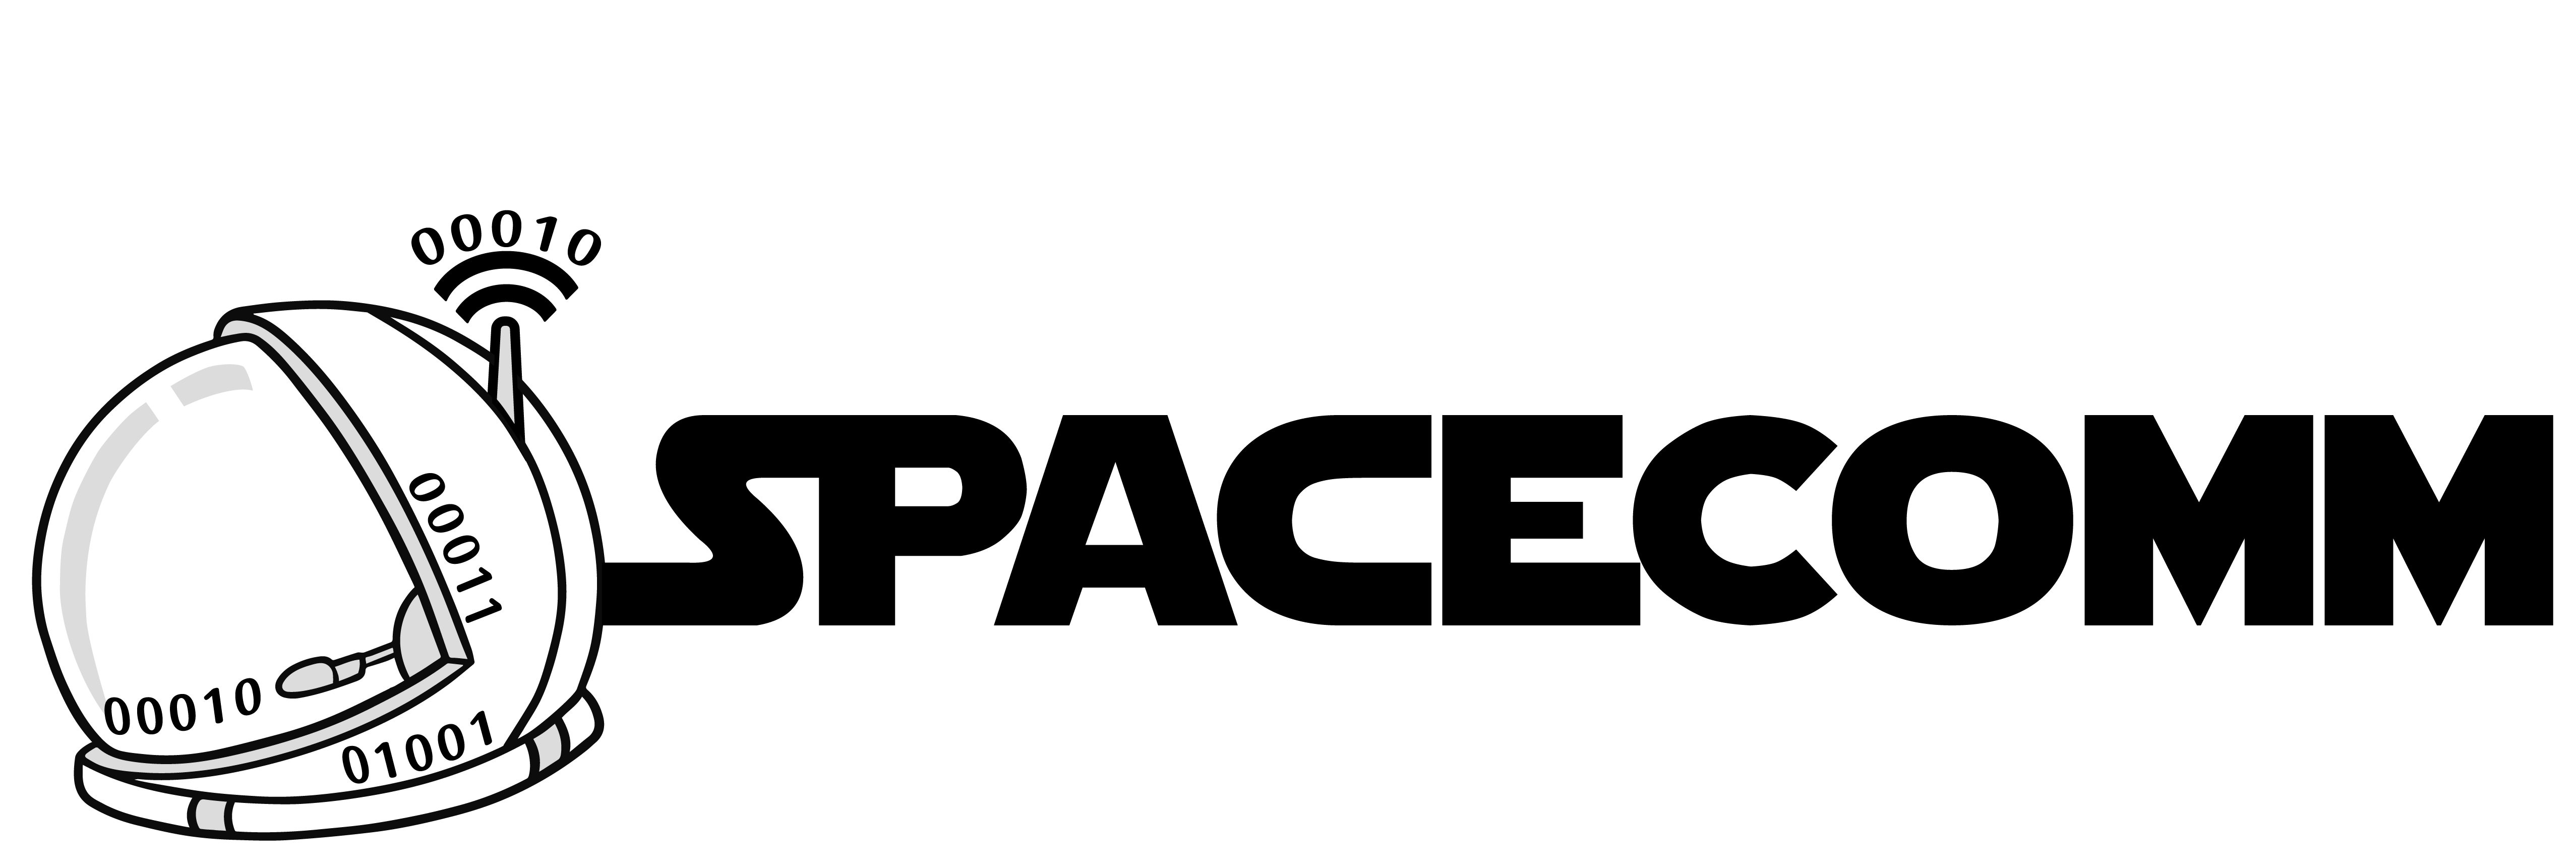
\includegraphics[keepaspectratio,width=1.2cm]{SpaceComm LOGO_Black_ Horizontal 1.png}}\hspace*{1ex}
        \end{beamercolorbox}%
    }%
    \vskip0pt% 確保之後的內容與這一部分緊密相連
}

% ------ 自定義尾部模板 ------
\setbeamertemplate{footline}{
    \leavevmode%
    \hbox{%
        \begin{beamercolorbox}[wd=.333333\paperwidth,ht=2.25ex,dp=1ex,center]{author in head/foot}%
            Chao-Yu Chen (EE/CCE, NCKU)
        \end{beamercolorbox}%
        \begin{beamercolorbox}[wd=.333333\paperwidth,ht=2.25ex,dp=1ex,center]{title in head/foot}%
            OFDM
        \end{beamercolorbox}%
        \begin{beamercolorbox}[wd=.333333\paperwidth,ht=2.25ex,dp=1ex,right]{date in head/foot}%
            \insertshortdate{}\hspace*{2em}
            \insertframenumber{} / \inserttotalframenumber\hspace*{2ex}
            % 加上頁碼與總頁數（其實我是計frame數因為pagenumber不會採計appendix的部份）
        \end{beamercolorbox}
    }%
    \vskip0pt%
}

% ------ Beamer 顏色設定 ------
\definecolor{Red}{RGB}{163,0,0} % 自定義紅色
\setbeamercolor{title}{fg=Red} % 設置標題顏色
\setbeamercolor{frametitle}{fg=Red} % 設置頁框標題顏色
\setbeamercolor{author in head/foot}{bg=Red, fg=white} % 設置頁眉頁腳中的作者顏色
\setbeamercolor{block title}{bg=red!30,fg=black} % 設置區塊標題顏色
\setbeamercolor{block body}{bg=blue!5,fg=black} % 設置區塊內容顏色
\setbeamercolor{caption name}{fg=black} % 設置標題名稱顏色
\setbeamercolor{bibliography item}{fg=black} % 設置參考文獻條目顏色
\setbeamercolor*{bibliography entry title}{fg=black} % 設置參考文獻標題顏色
\setbeamercolor*{bibliography entry author}{fg=black} % 設置參考文獻作者顏色
\setbeamercolor*{bibliography entry location}{fg=black} % 設置參考文獻位置顏色
\setbeamercolor*{bibliography entry note}{fg=black} % 設置參考文獻備註顏色


% ------ 參考文獻、項目、區塊和導航設定 ------
\setbeamertemplate{note page}[plain2] % 使用定義的備註頁模板
\setbeamertemplate{caption}[] % 圖片標題不帶有編號
%\setbeamertemplate{caption}[numbered] % 圖片標題帶有編號
\setbeamertemplate{bibliography item}[text] % 參考文獻條目模板
\setbeamertemplate{blocks}[rounded][shadow=true] % 區塊有圓角和陰影
\setbeamertemplate{navigation symbols}{} % 不顯示導航符號


% ------ 項目符號設定 ------
\setbeamertemplate{items}[circle] % 項目符號為球體
\setbeamercolor{itemize item}{fg=black} % 設置一級項目符號顏色
\setbeamercolor{itemize subitem}{fg=black} % 設置二級項目符號顏色
\setbeamercolor{itemize subsubitem}{fg=black} % 設置三級項目符號顏色


% ------ 新命令 ------
\newcommand{\Fig}{Fig.$\,$} % 簡化圖片引用
\newcommand{\Acal}{\mathcal A} % 簡化數學符號
\newcommand{\nn}{\nonumber} % 簡化數學符號
\newcommand{\E}{{\mathrm{E}}} % 簡化數學符號
\newcommand{\PAPR}{\mbox{PAPR}} % 簡化數學符號

\newcommand{\Nshift}{$N-$shift auto-orthogonal } % 簡化特定術語
\newcommand{\auto}{autocorrelation } % 簡化特定術語
\newcommand{\cross}{cross-correlation } % 簡化特定術語
\newcommand{\highlight}[1]{\textbf{\textcolor{Red}{#1}}} % 定義一個新命令來加粗和染色文字

% ------ 定理、定義、性質等環境 ------
\newtheorem{thm}{Theorem} % 定義定理環境
\newtheorem{rmk}{Remark} % 定義備註環境
\newtheorem{prop}[thm]{Proposition} % 定義命題環境
\newtheorem{property}[thm]{Property} % 定義性質環境
\newtheorem{defin}{Definition} % 定義定義環境
\newtheorem{crly}{Corollary} % 定義推論環境
\newtheorem{eg}{Example} % 定義示例環境
\newtheorem{remark}{Remark} % 定義備註環境
%\newtheorem{lemma}{Lemma}

% 重新定義腳註樣式
\renewcommand{\thefootnote}{\fnsymbol{footnote}}

%--------------------讓作者裡面可以加換行符號-----------------------------------%
\pdfstringdefDisableCommands{%
  \def\\{}%
  \def\texttt#1{<#1>}%
}

%-----------------------------------開始--------------------------------------%
\title{Introduction to Orthogonal Frequency Division Multiplexing (OFDM) Technique}
\author{\large 湯庭豐、邊任祥、張景翔、黃智筠\\李星樺、劉家瑋、陳品蓉}
\institute{\large 國立成功大學\\通訊工程研究所}
\titlegraphic{\vspace{-2cm}\hspace{10cm}
\includegraphics[width=2cm]{ncku_logo.jpg}
}
\date{\today}
\begin{document}

%-----------------------------------------------------------------------------%
\begin{frame}
    \titlepage
\end{frame}


%-----------------------------------------------------------------------------%
\begin{frame}
    \frametitle{Outline}
    \begin{itemize}
        \item OFDM Overview
        \item OFDM System Model
        \item Orthogonality
        \item Multi-Carrier Equivalent Implementation by Using IDFT (IFFT)
        \item Cyclic Prefix (CP)
        \item Summary
    \end{itemize}
\end{frame}
%-----------------------------------------------------------------------------%
\begin{frame}
    \frametitle{Transmission Mode}
    \begin{itemize}
        \item Single-Carrier (SC) vs. Multi-Carrier (MC)
    \end{itemize}
    \begin{figure}
        \centering
        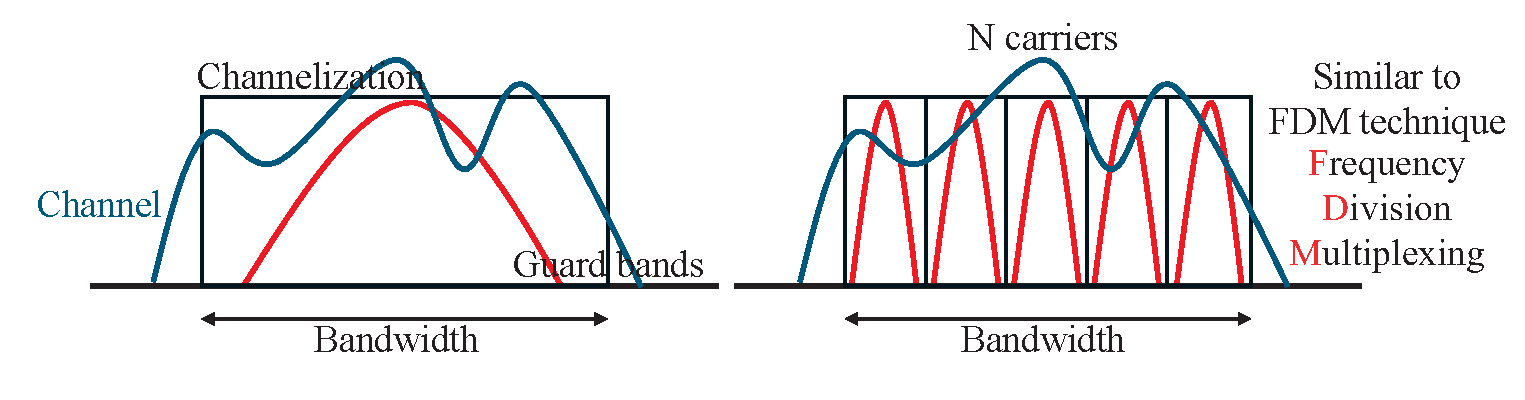
\includegraphics[width=0.99\textwidth]{SC_MC.eps}
    \end{figure}
    \begin{minipage}[t]{0.49\textwidth}
        \begin{itemize}
            \item Data are transmitted over only one carrier.
            \item Frequency selective fading.
        \end{itemize}
    \end{minipage} 
    \begin{minipage}[t]{0.49\textwidth}
        \begin{itemize}
            \item Data are shared among several carriers and simultaneously transmitted.
            \item Flat fading.
        \end{itemize}
    \end{minipage} 
\end{frame}
%----------------------------------------------------------------------------%
\begin{frame}
    \frametitle{OFDM Definition}
    \begin{itemize}
        \item OFDM
        \begin{itemize}
            \item \highlight{O}rthogonal \highlight{F}requency \highlight{D}ivision \highlight{M}ultiplexing
        \end{itemize}
    \end{itemize}
    \begin{itemize}
        \item The basic principle of OFDM is to \highlight{split a high-rate data \\stream into a number of lower rate streams} that are\\ transmitted simultaneously over a number of sub-carriers.
        \item It eliminates or alleviates the problem of \highlight{multi-path channel fading effect}, \highlight{low spectrum efficiency}, and \highlight{frequency selective fading}.
    \end{itemize}
\end{frame}
%----------------------------------------------------------------------------%
\begin{frame}
    \frametitle{OFDM Overview(1/2)}
    \begin{itemize}
        \item OFDM modulation
    \end{itemize}
    \begin{figure}
        \centering
        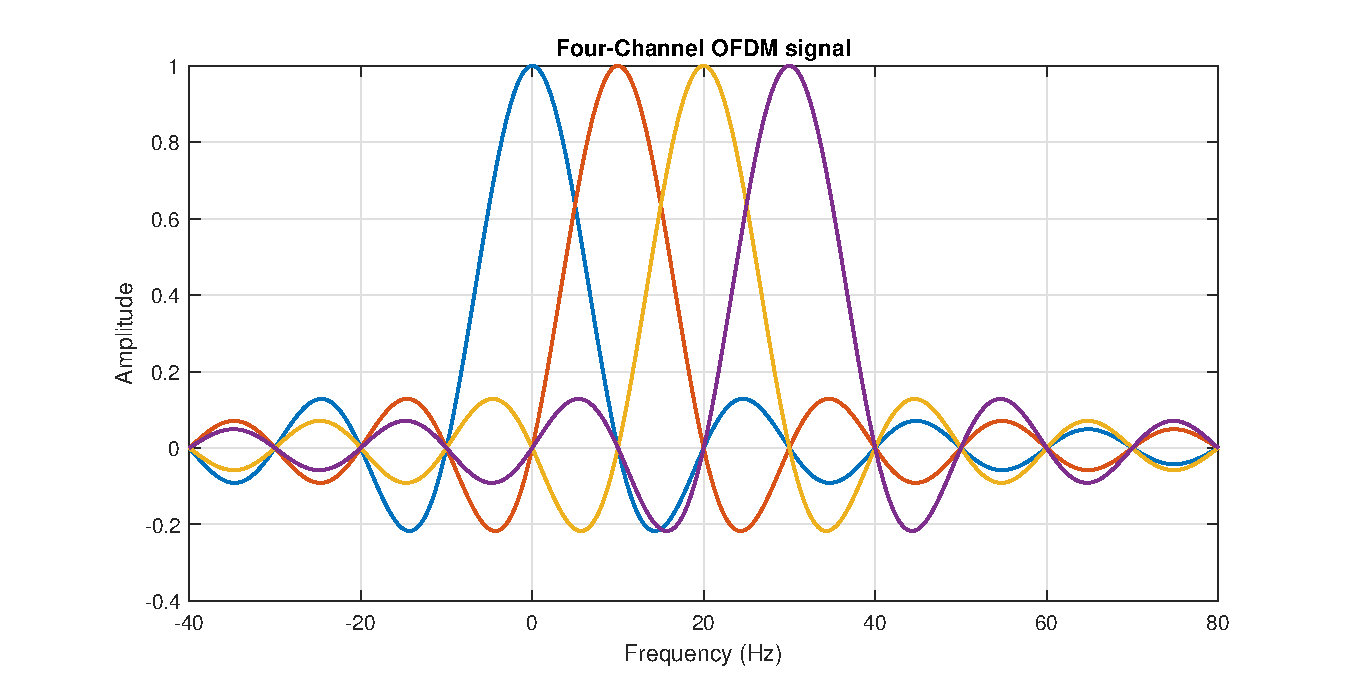
\includegraphics[width=0.9\textwidth]{OFDM_signal.eps}
    \end{figure}
\end{frame}
%----------------------------------------------------------------------------%
\begin{frame}
    \frametitle{OFDM Overview(2/2)}
    \begin{itemize}
        \setlength{\itemsep}{8pt}
        \item Feature
        \begin{itemize}
            \setlength{\itemsep}{8pt}
            \item No intercarrier guard bands
            \item Overlapping of bands
            \item Spectral efficiency
            \item Easy implementation by IFFTs
            \item Very sensitive to synchronization
        \end{itemize}
    \end{itemize}
\end{frame}
%----------------------------------------------------------------------------%
\begin{frame}
    \frametitle{OFDM Transmitter}
    \begin{figure}
        \centering
        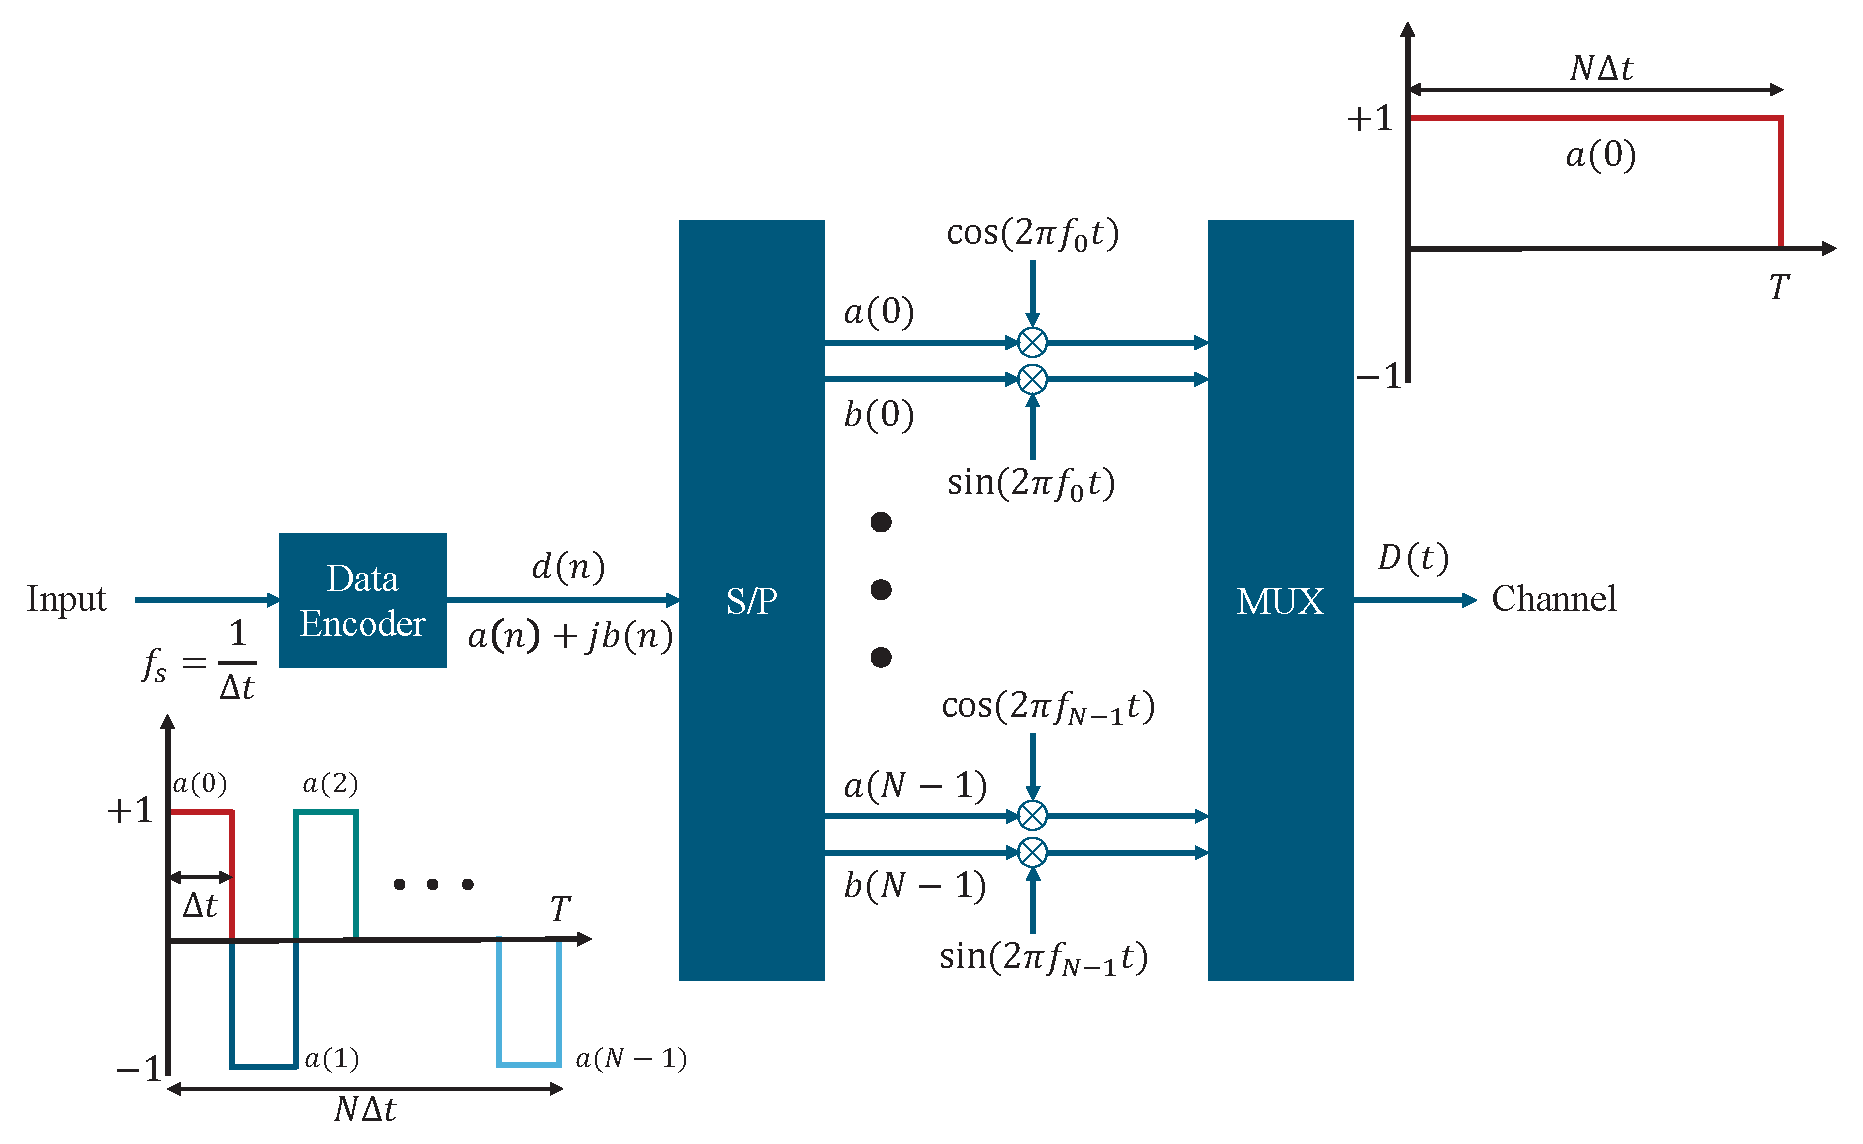
\includegraphics[width=0.9\textwidth]{transmitter.eps}
    \end{figure}
\end{frame}
%----------------------------------------------------------------------------%
\begin{frame}
    \frametitle{Multi-carrier Systems}
    \begin{itemize}
        \item Multi-carrier Transmission
    \end{itemize}
    \begin{figure}
        \centering
        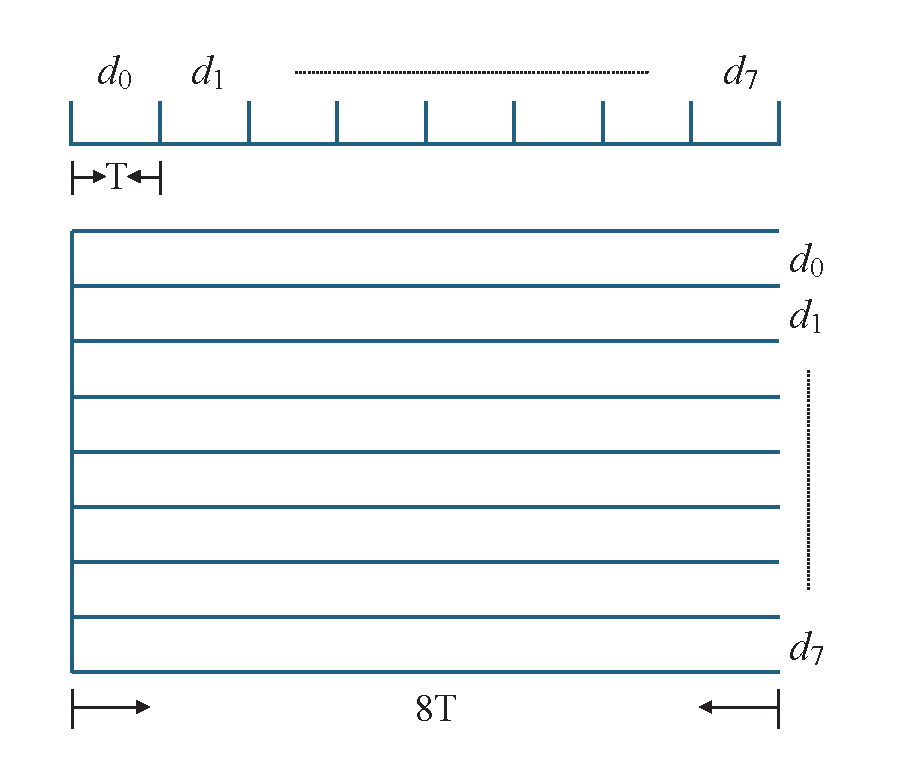
\includegraphics[width=0.65\textwidth]{MC_System.eps}
    \end{figure}
\end{frame}
%----------------------------------------------------------------------------%
\begin{frame}
    \frametitle{Multi-carrier Systems}
    \begin{itemize}
        \item Multi-carrier for ${N=8}$
    \end{itemize}
    \begin{minipage}{0.45\textwidth}
        \begin{figure}
            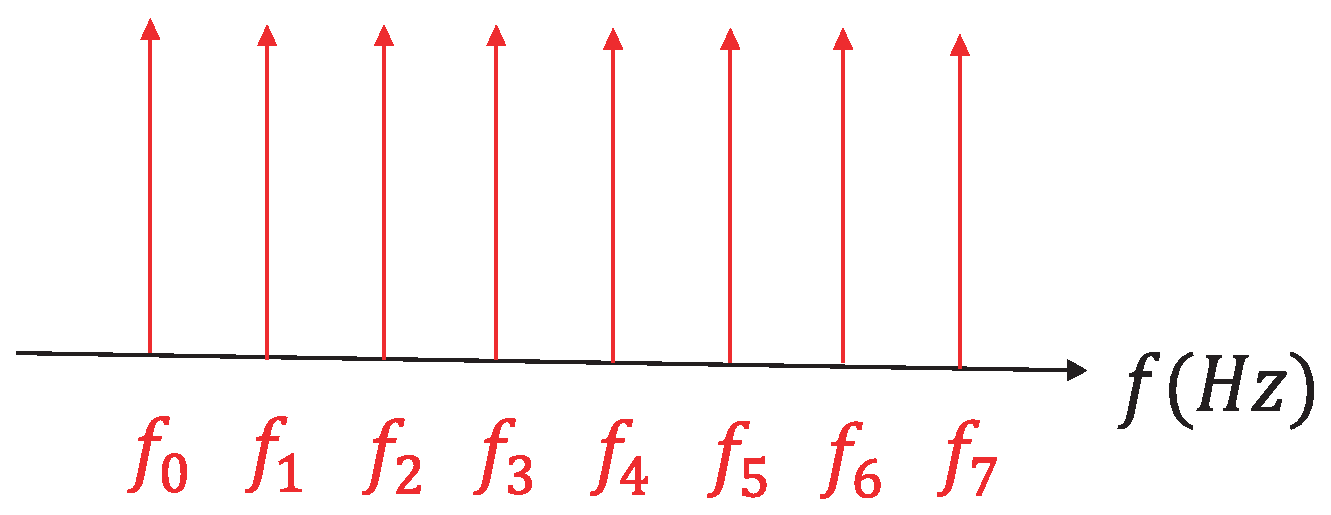
\includegraphics[width=0.99\textwidth]{subcarrier.eps}
        \end{figure}
    \end{minipage}
    \begin{minipage}{0.45\textwidth}
        \begin{align*}
            \delta(f - f_0) & \longrightarrow \exp(j 2\pi f_0 t) \\
            \delta(f - f_1) & \longrightarrow \exp(j 2\pi f_1 t) \\
            \delta(f - f_2) & \longrightarrow \exp(j 2\pi f_2 t) \\
            \delta(f - f_3) & \longrightarrow \exp(j 2\pi f_3 t) \\
            \delta(f - f_4) & \longrightarrow \exp(j 2\pi f_4 t) \\
            \delta(f - f_5) & \longrightarrow \exp(j 2\pi f_5 t) \\
            \delta(f - f_6) & \longrightarrow \exp(j 2\pi f_6 t) \\
            \delta(f - f_7) & \longrightarrow \exp(j 2\pi f_7 t) \\
        \end{align*}
    \end{minipage}
\end{frame}
%----------------------------------------------------------------------------%
\begin{frame}
    \frametitle{Transmitted Signal (1/4)}
    \begin{itemize}
        \item The transmitted waveform ${D(t)}$ can be proved as
        \begin{align*}
            D(t) &= Re\Big\{\sum_{n=0}^{N-1} d(n) \exp(j2\pi f_{n} t)\Big\} \\
            &=Re\Big\{\sum_{n=0}^{N-1}\ [a(n)+jb(n)][\cos{(2\pi f_{n}t)}+j\sin{(2\pi f_{n}t)}]\Big\}\\
            &=\sum_{n=0}^{N-1}\ a(n)\cos{(2\pi f_{n}t)}-b(n)\sin{(2\pi f_{n}t)}
        \end{align*}
    \end{itemize}
\end{frame}
%----------------------------------------------------------------------------%
\begin{frame}
    \frametitle{Transmitted Signal (2/4)}
    \begin{itemize}
        \item The transmitted waveform ${D(t)}$ can be expressed as
        \begin{equation} \label{a}
            D(t)=\sum_{n=0}^{N-1}\{a(n)\cos{(2{\pi}f_{n}t)}+b(n)\sin{(2{\pi}f_{n}t)}\}
        \end{equation}
        \[\text{where}\ f_{n}=f_{0}+n\Delta{f}\ \text{and}\ \Delta{f}=\frac{1}{N\Delta{t}}\]
        %\begin{itemize}
            \item Using a two-dimensional digital modulation format, the data
	              symbols $d(n)$ can be represented as $a(n) + jb(n)$.
            \begin{itemize}
                \item $a(n)$ : in-phase component
                \item $b(n)$ : quadrature component
            \end{itemize}
        %\end{itemize}
    \end{itemize}
\end{frame}
%----------------------------------------------------------------------------%
\begin{frame}
    \frametitle{Transmitted Signal (3/4)}
        \centering
        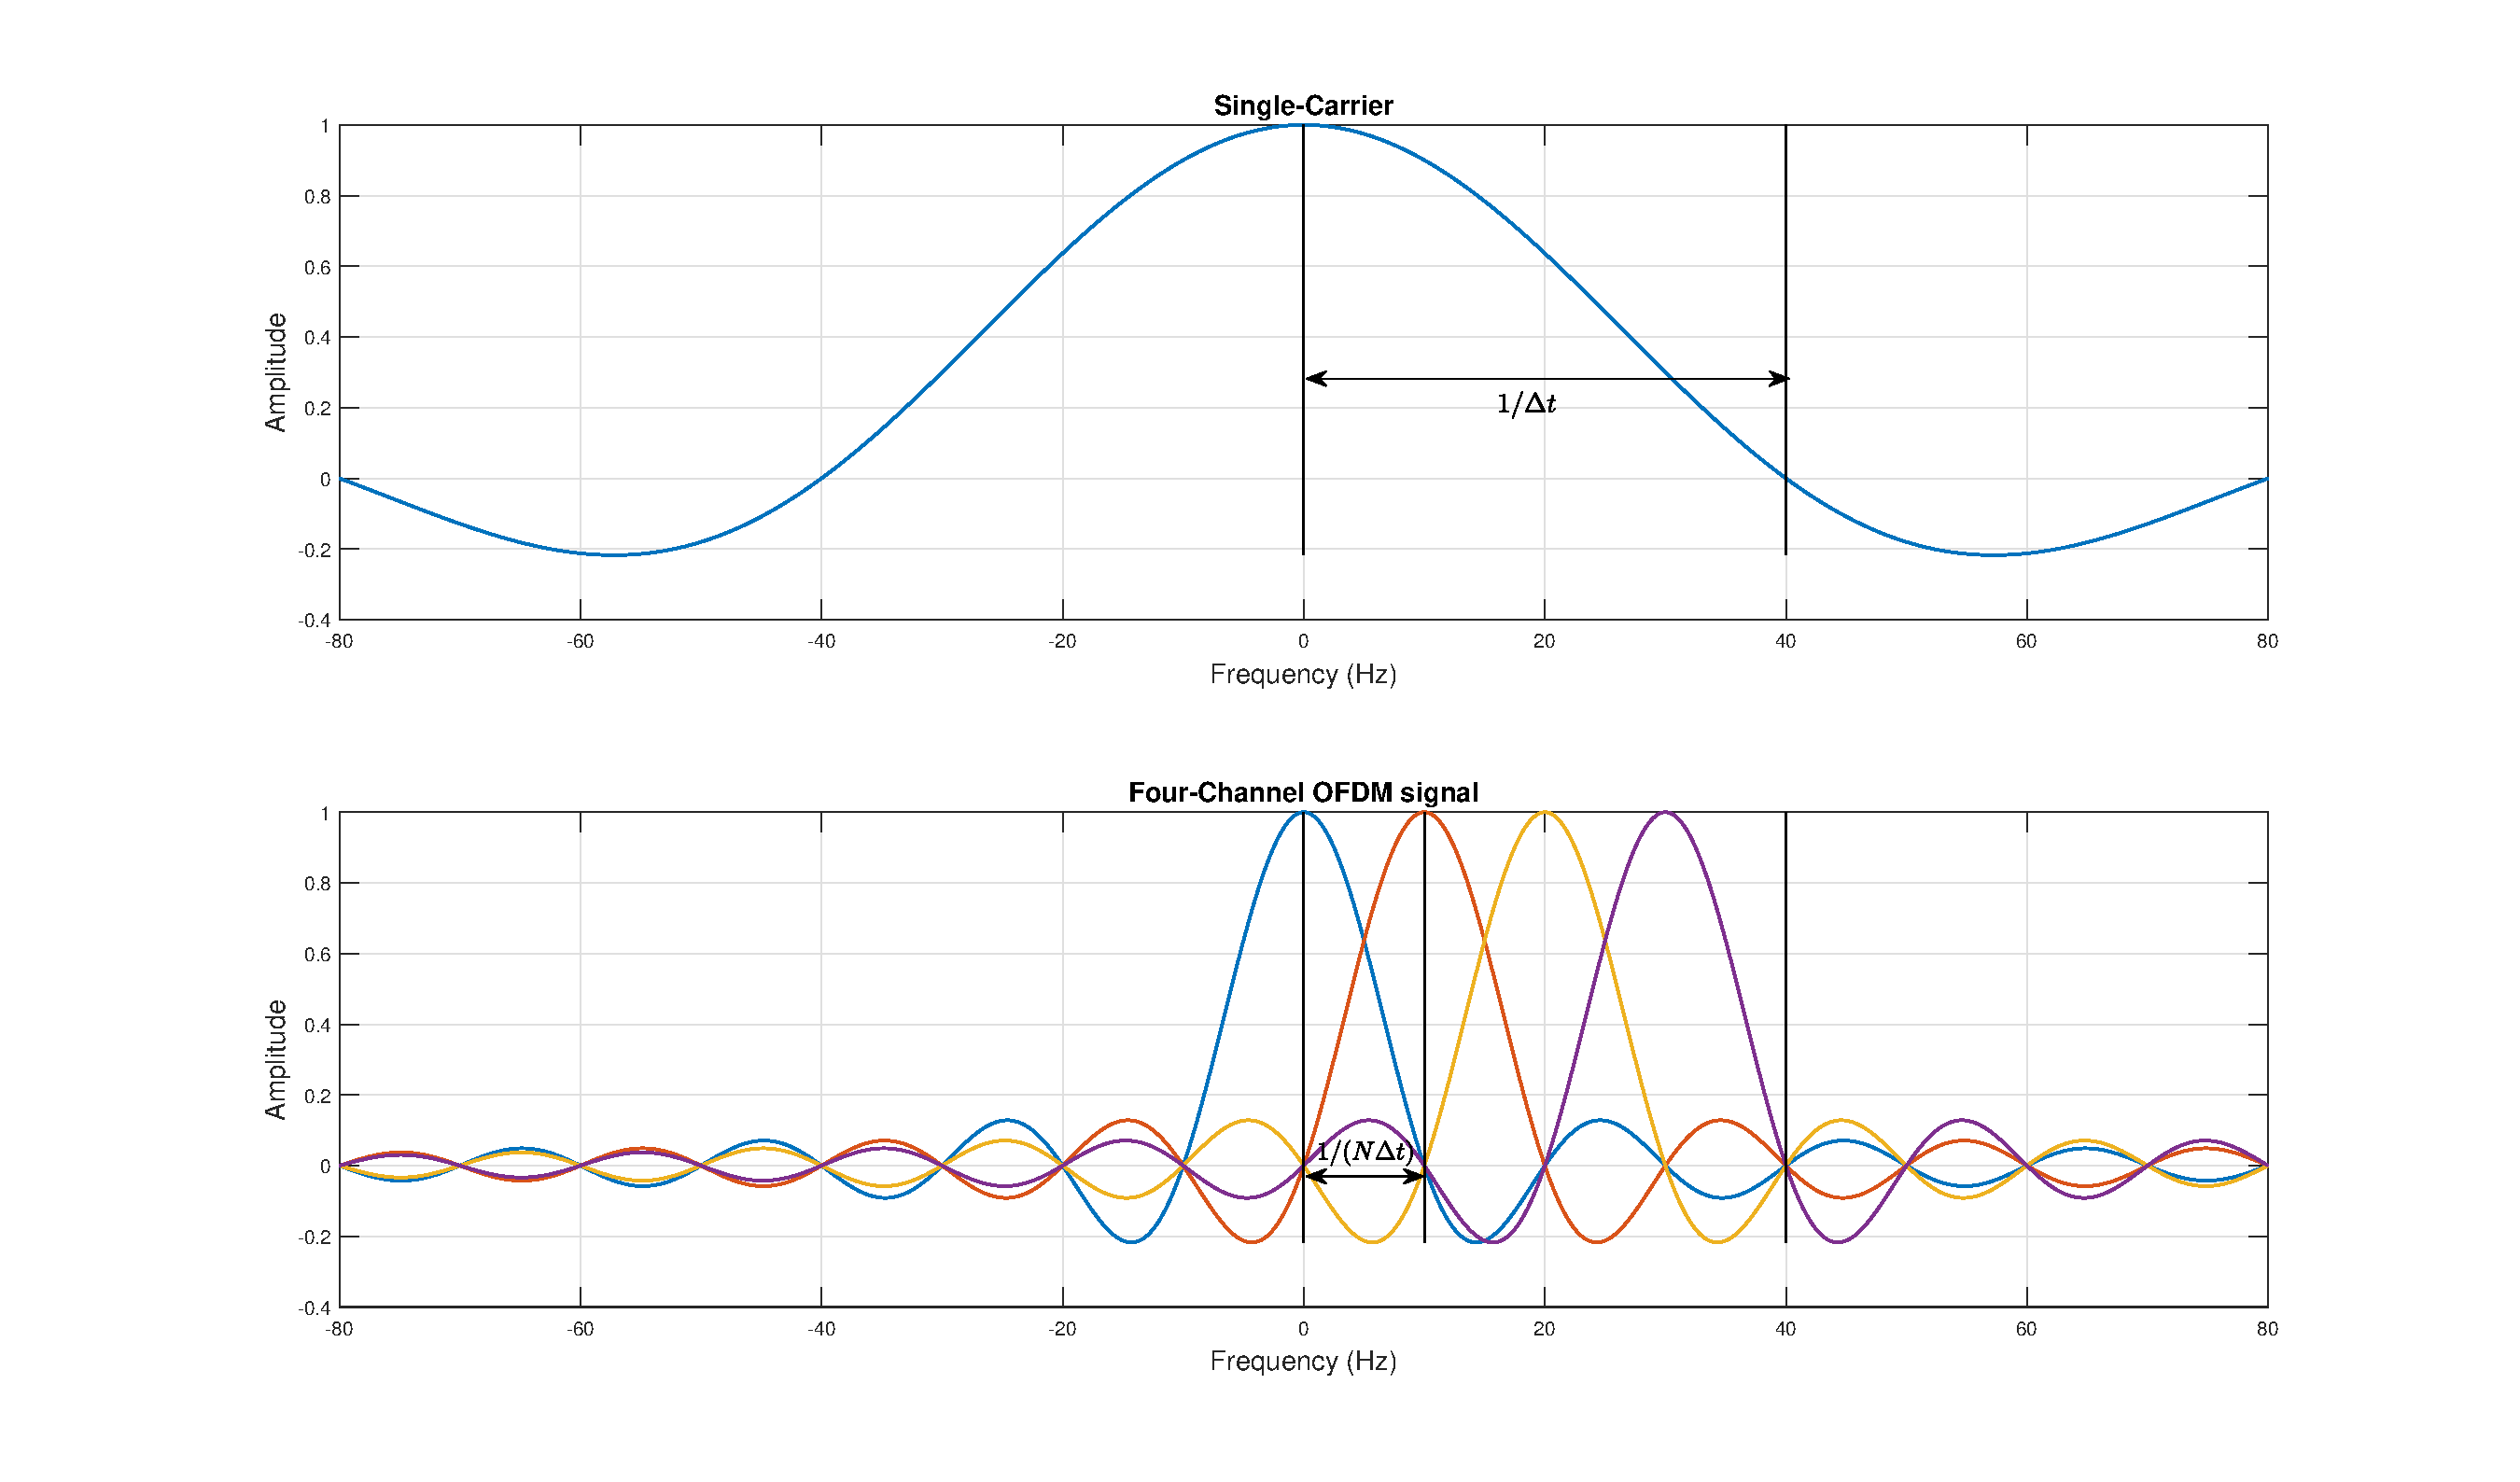
\includegraphics[width=0.9\textwidth]{delta_f.eps}
\end{frame}
%----------------------------------------------------------------------------%
\begin{frame}
    \frametitle{Transmitted Signal (4/4)}
        \begin{figure}
        \centering
            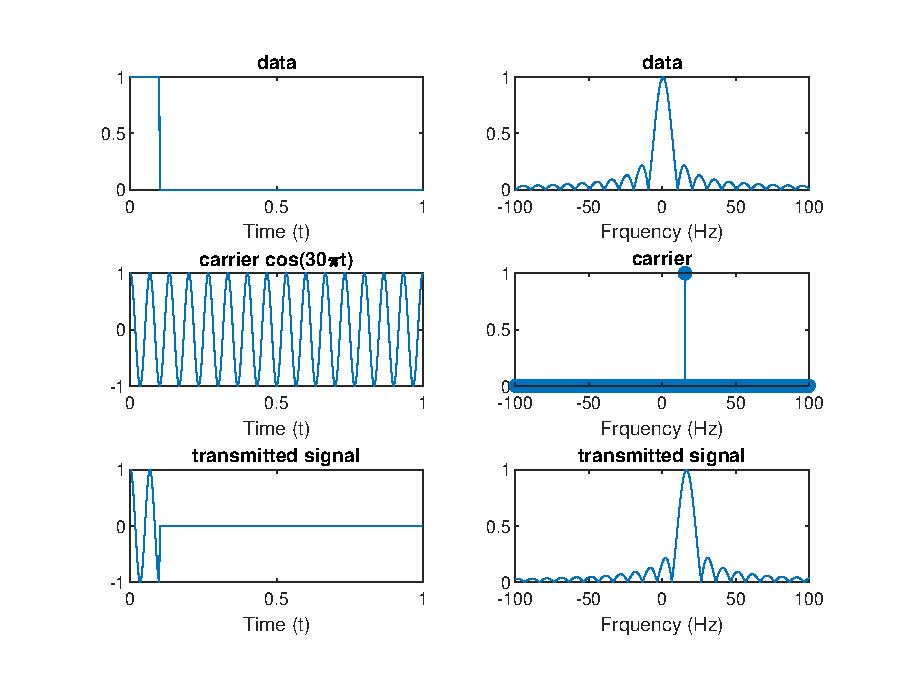
\includegraphics[width=0.8\textwidth]{sc.eps}
        \end{figure}
\end{frame}
%----------------------------------------------------------------------------%
\begin{frame}
    \frametitle{OFDM System Model}
    \begin{itemize}
        \item The serial data elements spaced by $\Delta{t}$ are grouped and used to modulate N carriers. Thus they are frequency division multiplexed.
        \item The signaling interval is then increased to $N\Delta{t}$, which makes the system less susceptible to channel delay spread impairments.
    \end{itemize}
    \begin{figure}
        \centering
        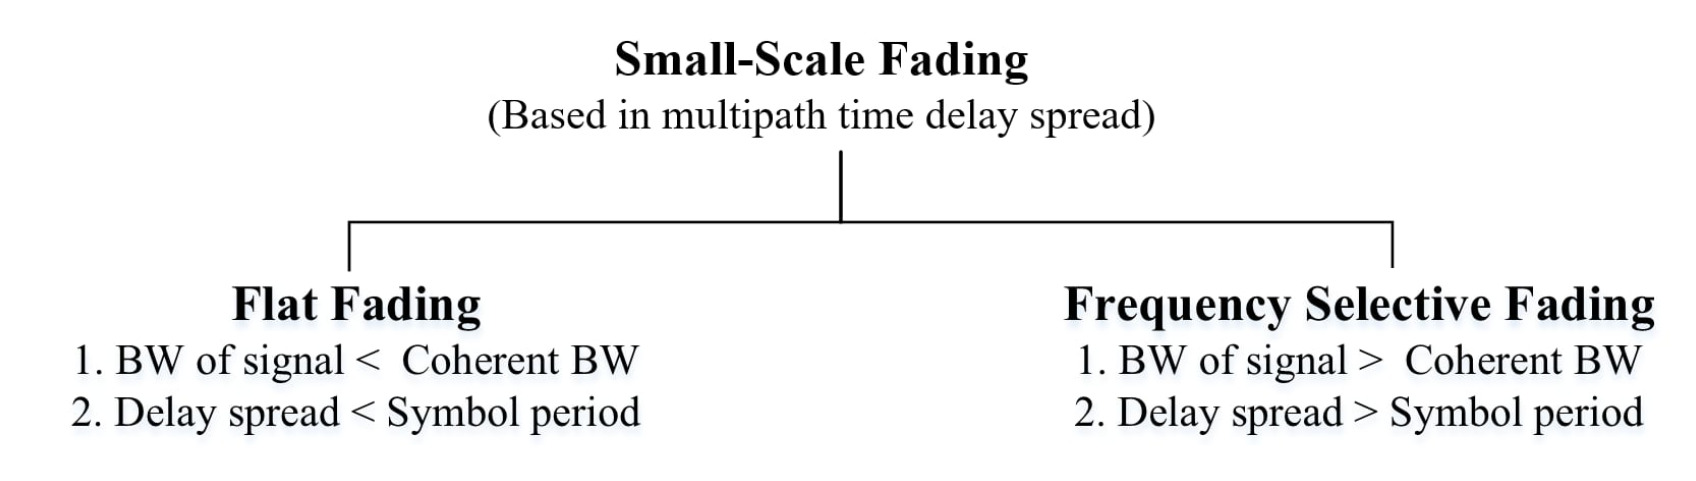
\includegraphics[width=0.75\textwidth]{e04su3su;6.jpg}
        %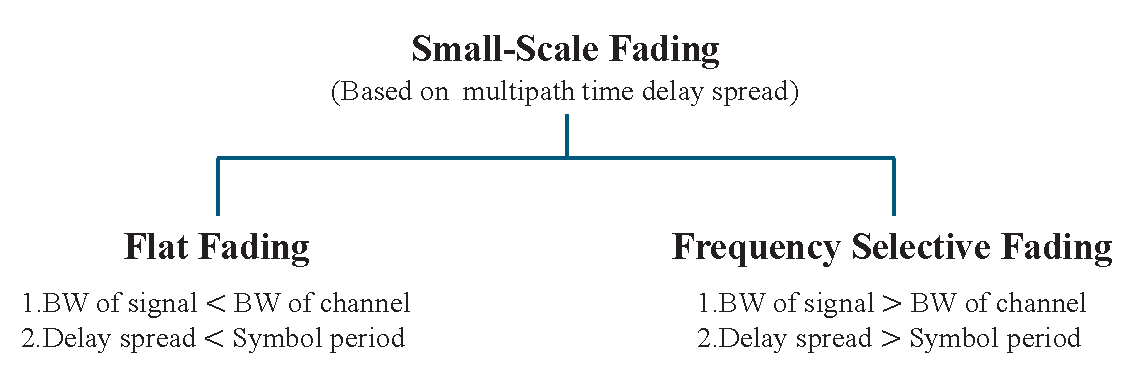
\includegraphics[width=0.75\textwidth]{fading.eps}
    \end{figure}
\end{frame}
%----------------------------------------------------------------------------%
\begin{frame}
    \frametitle{Symbol Period vs. Multipath Interference}
    \begin{itemize}
        \item Under the same multipath delay condition, as the symbol period lengthens, the impact of multipath interference decreases.
    \end{itemize}
    \begin{figure}
        \centering
        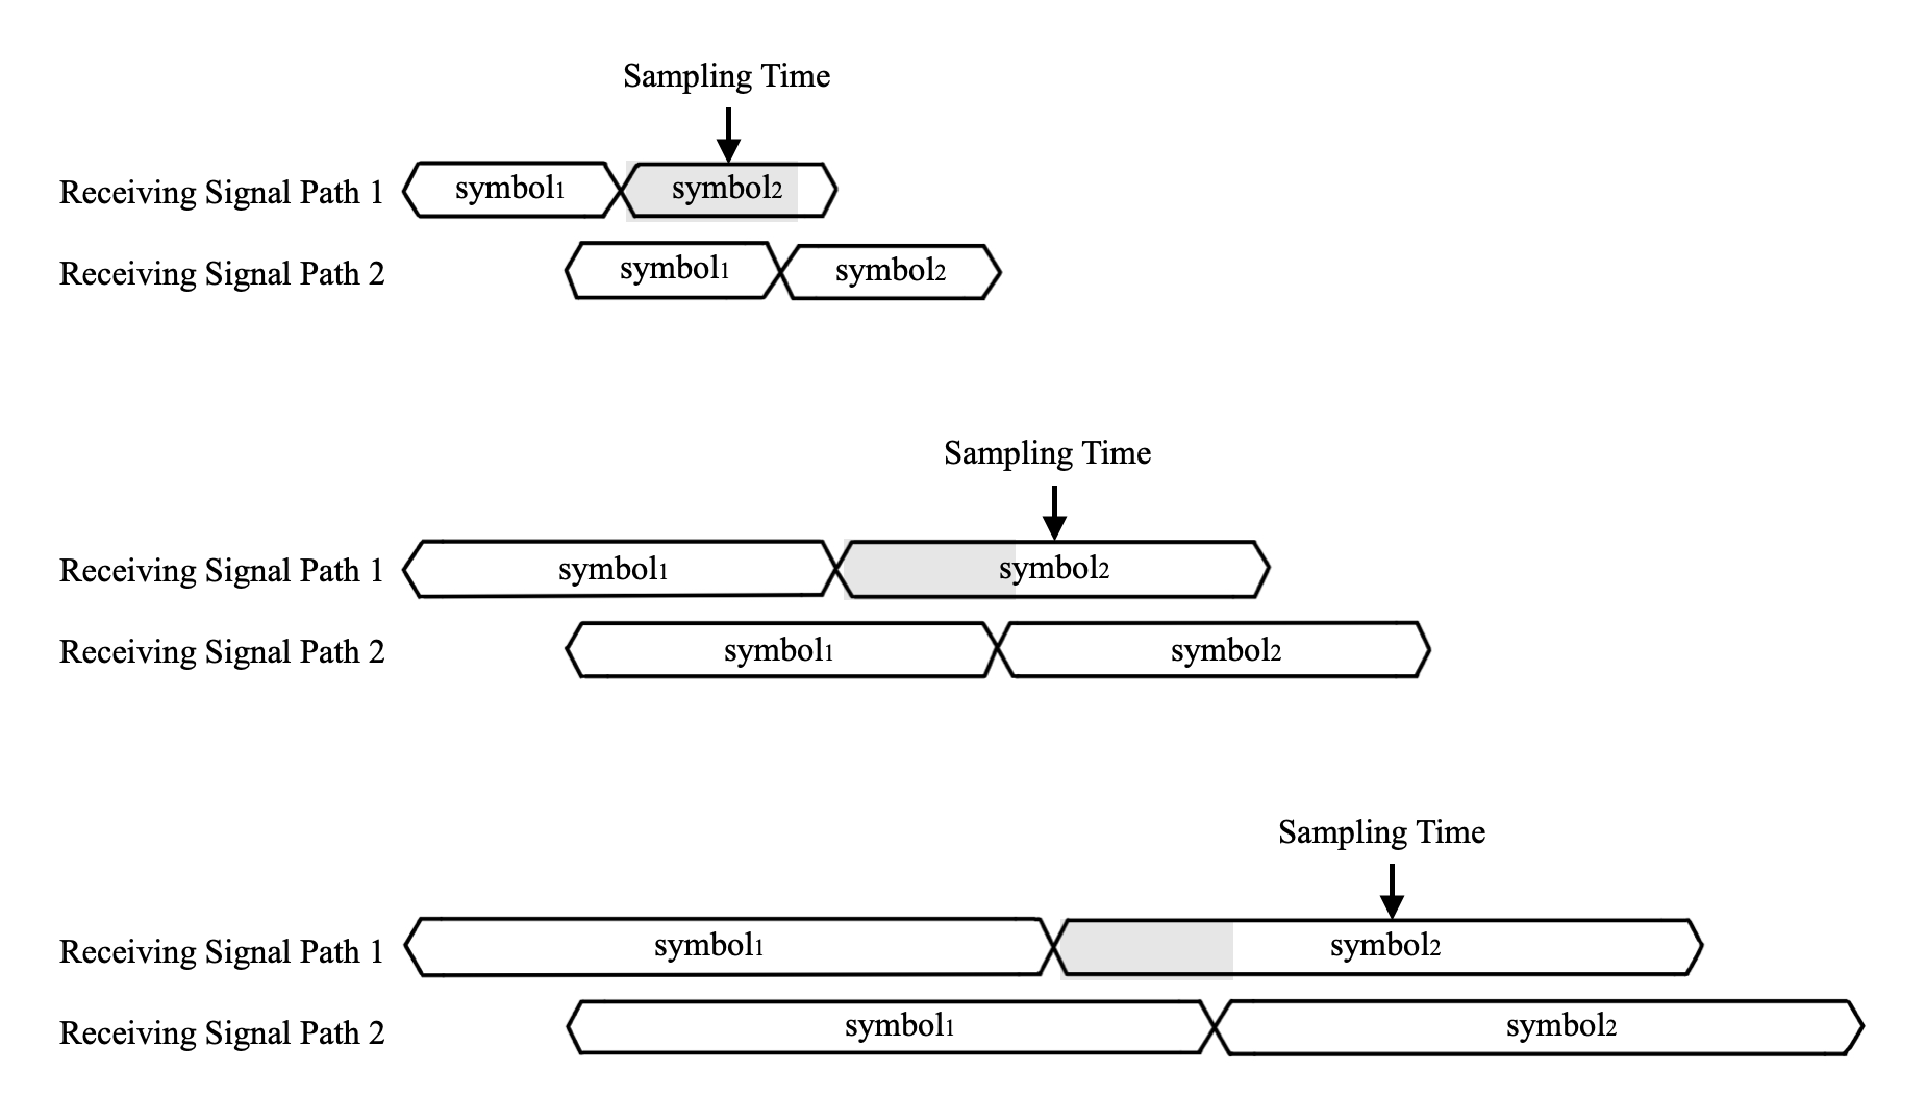
\includegraphics[width=0.75\textwidth]{Delay_SymbolTime.eps}
    \end{figure}
\end{frame}
%----------------------------------------------------------------------------%
\begin{frame}
    \frametitle{Multipath propagation (1/8)}
    \begin{itemize}
        \item Multipath is the propagation phenomenon that results in radio signals reaching the receiving antenna by two or more paths.
    \end{itemize}
    \begin{figure}
        \centering
        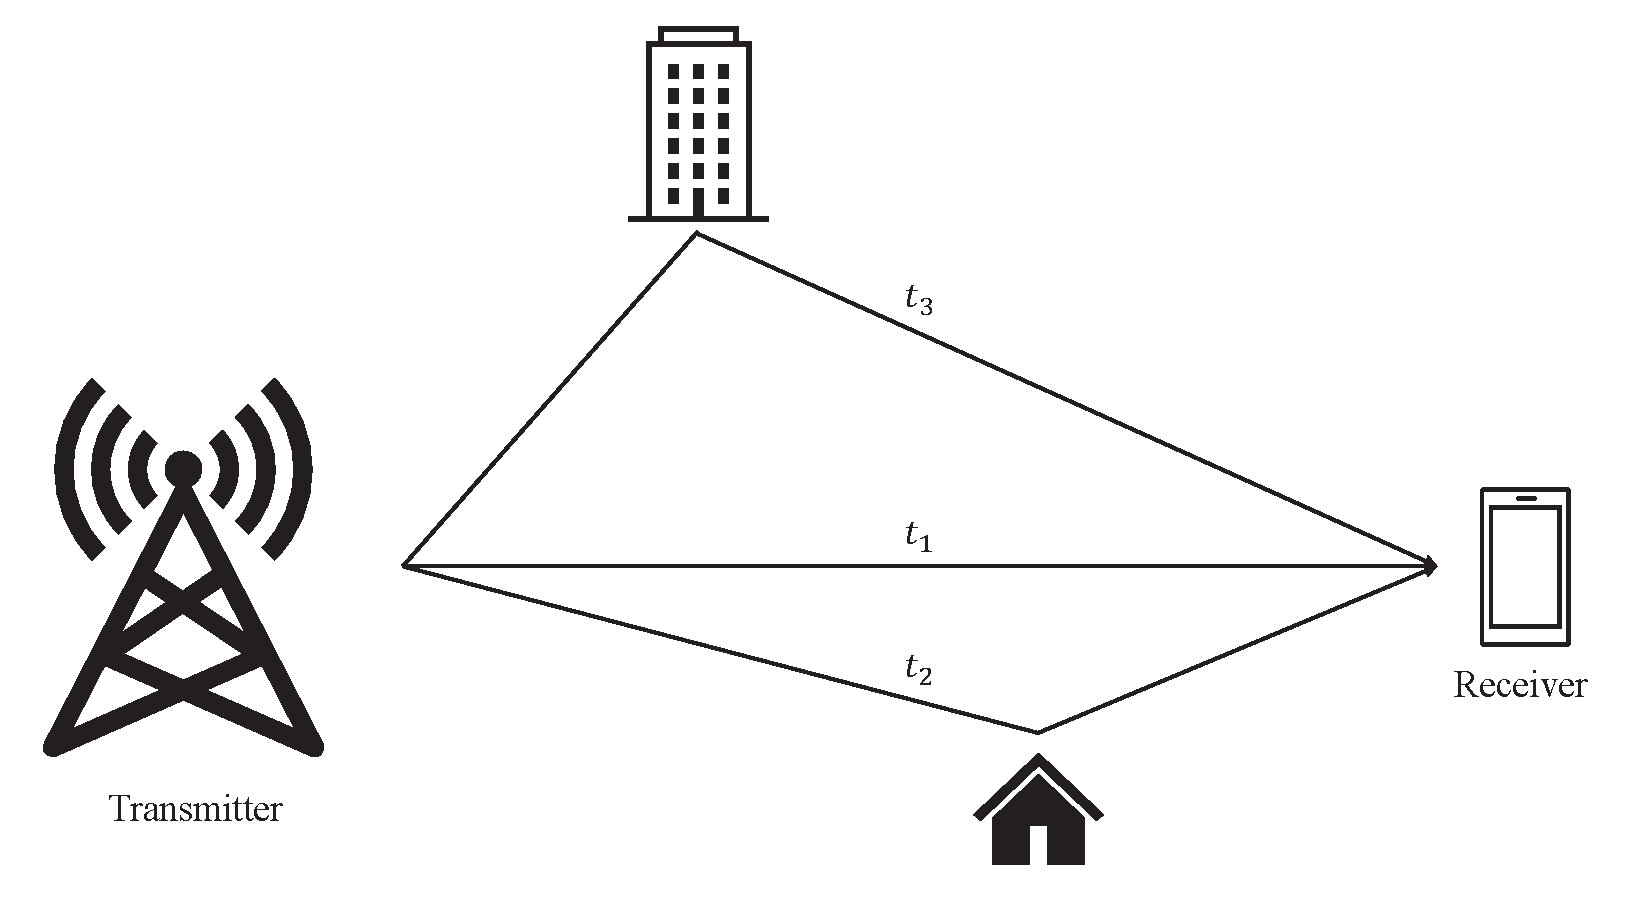
\includegraphics[width=0.75\textwidth]{Multipath_propagation.eps}
    \end{figure}
\end{frame}
%----------------------------------------------------------------------------%
\begin{frame}
    \frametitle{Multipath propagation (2/8)}
    \begin{itemize}
        \item Multipath propagation results in a received signal that is dispersed in time.
    \end{itemize}
    \begin{figure}
        \centering
        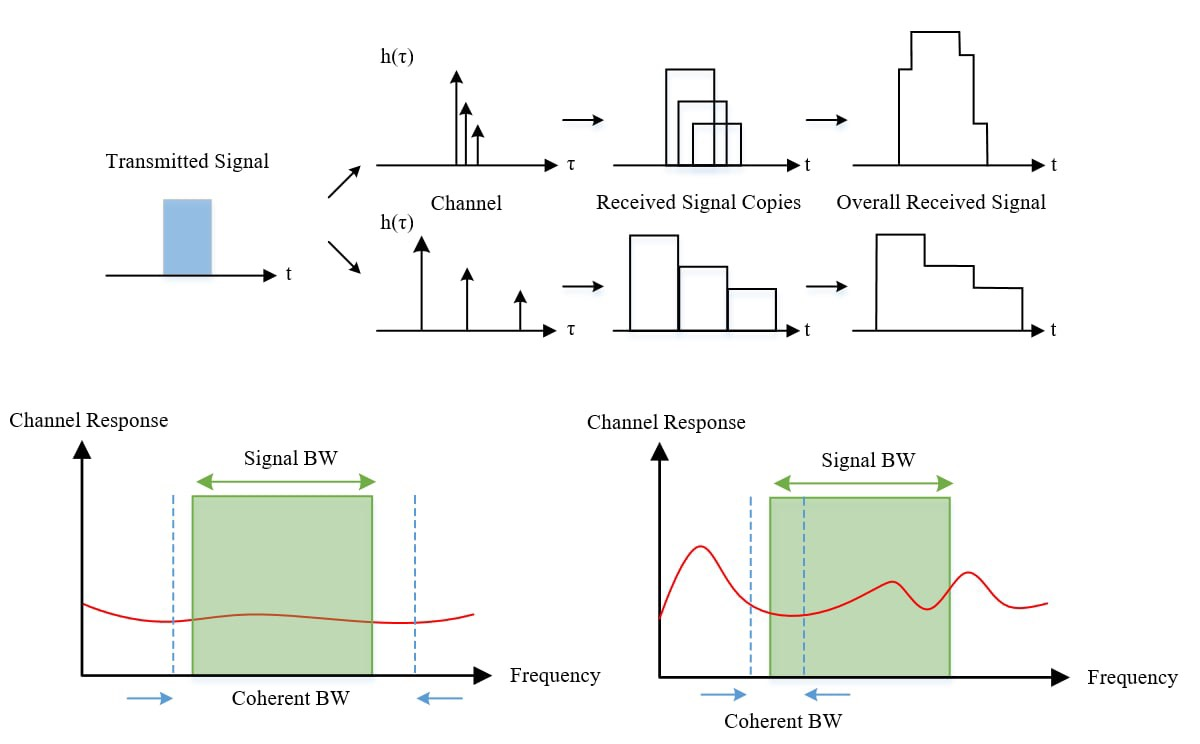
\includegraphics[width=0.75\textwidth]{multipath_2.jpg}
        %original fig: Delay_spread.eps%
    \end{figure}
\end{frame}
%----------------------------------------------------------------------------%
\begin{frame}
    \frametitle{Multipath propagation (3/8) --- Proof}
    \begin{itemize}
        \item Two-path channel impulse response:
        \begin{align*}
            &h(t)=a\delta(t)+b\delta(t-\tau) \\
            &\text{where } a \text{ and } b \text{ are the amplitudes, and }
            \tau \text{ is the delay of the second path.}
        \end{align*}
    \end{itemize}
    \begin{itemize}
        \item Frequency response:
        \begin{align*}
            H(f)&=a+b e^{-j 2\pi f \tau} \\
            \left| H(f) \right|^2&=H(f)H(f)^*\\
            &=(a+b e^{-j 2\pi f \tau})(a+b e^{j 2\pi f \tau})\\
            &=a^2+ab(e^{-j 2\pi f \tau} + e^{j 2\pi f \tau})+b^2\\
            &=a^2+ab \cdot 2\cos(2\pi f \tau) +b^2\\
            &=a^2+b^2+2ab\cos(2\pi f \tau)\\
        \end{align*}
    \end{itemize}
\end{frame}
%----------------------------------------------------------------------------%
\begin{frame}
    \frametitle{Multipath propagation (4/8) --- Proof}

    \begin{itemize}
        \item N-path channel impulse response:
        \begin{align*}
            h(t)
            &= \sum_{n=0}^{N-1}
            a_n \delta(t-\tau_n) \\
            &\text{where } a_n \text{ is the amplitude of the }n\text{-th path,}\\
            &\tau_n \text{ is the delay of the }n\text{-th path.}
        \end{align*}
    \end{itemize}

    \begin{itemize}
        \item Frequency response:
        \begin{align*}
            H(f)
            &= \sum_{n=0}^{N-1}
            a_n e^{-j2\pi f\tau_n} \\[2mm]
            |H(f)|^2
            &= H(f)H(f)^* \\
            &=
            \left(
            \sum_{n=0}^{N-1}
            a_n e^{-j2\pi f\tau_n}
            \right)
            \left(
            \sum_{m=0}^{N-1}
            a_m e^{j2\pi f\tau_m}
            \right).
        \end{align*}
    \end{itemize}
\end{frame}
%----------------------------------------------------------------------------%
\begin{frame}
    \frametitle{Multipath propagation (5/8) --- Proof}

    \begin{itemize}
        \item Continued from previous page:
        \begin{align*}
            &=
            \sum_{n=0}^{N-1}
            \sum_{m=0}^{N-1}
            a_n a_m
            e^{-j2\pi f(\tau_n-\tau_m)} \\
            &=
            \sum_{n=0}^{N-1} a_n^2
            +
            2\sum_{n=0}^{N-2}
            \sum_{m=n+1}^{N-1}
            a_n a_m
            \cos\left(
            2\pi f(\tau_n-\tau_m)
            \right).
        \end{align*}
    \end{itemize}
\end{frame}

%----------------------------------------------------------------------------%
\begin{frame}
    \frametitle{Multipath propagation (6/8) --- Proof}
    \begin{itemize}
        \item $a = b$.
        \begin{align*}
            \left| H(f) \right|^2 &= a^2 + a^2 + 2a^2\cos(2\pi f \tau) \\
            &= 2a^2 \left(1+\cos(2\pi f \tau)\right) \\
        \end{align*}
        If $\cos(2 \pi f \tau) = -1$, then signal cancellation.

        \item $a \neq b$.
        \begin{align*}
            \left| H(f) \right|^2 &= a^2 + b^2 + 2ab\cos(2\pi f \tau)
        \end{align*}
        Although $\cos(2 \pi f \tau) = -1$, signal is not cancellation.
        \begin{align*}
            {\left| H(f) \right|_{\min}}^2 &= a^2 + b^2 - 2ab = (a-b)^2 \\
            \left| H_{\min} \right| &= \left| a-b \right| \neq 0
        \end{align*}
    \end{itemize}
\end{frame}
%----------------------------------------------------------------------------%
\begin{frame}
    \frametitle{Multipath propagation (7/8)}
    \begin{itemize}
        \item Two paths, each with a different amplitude.
    \end{itemize}
    \begin{figure}
        \centering
        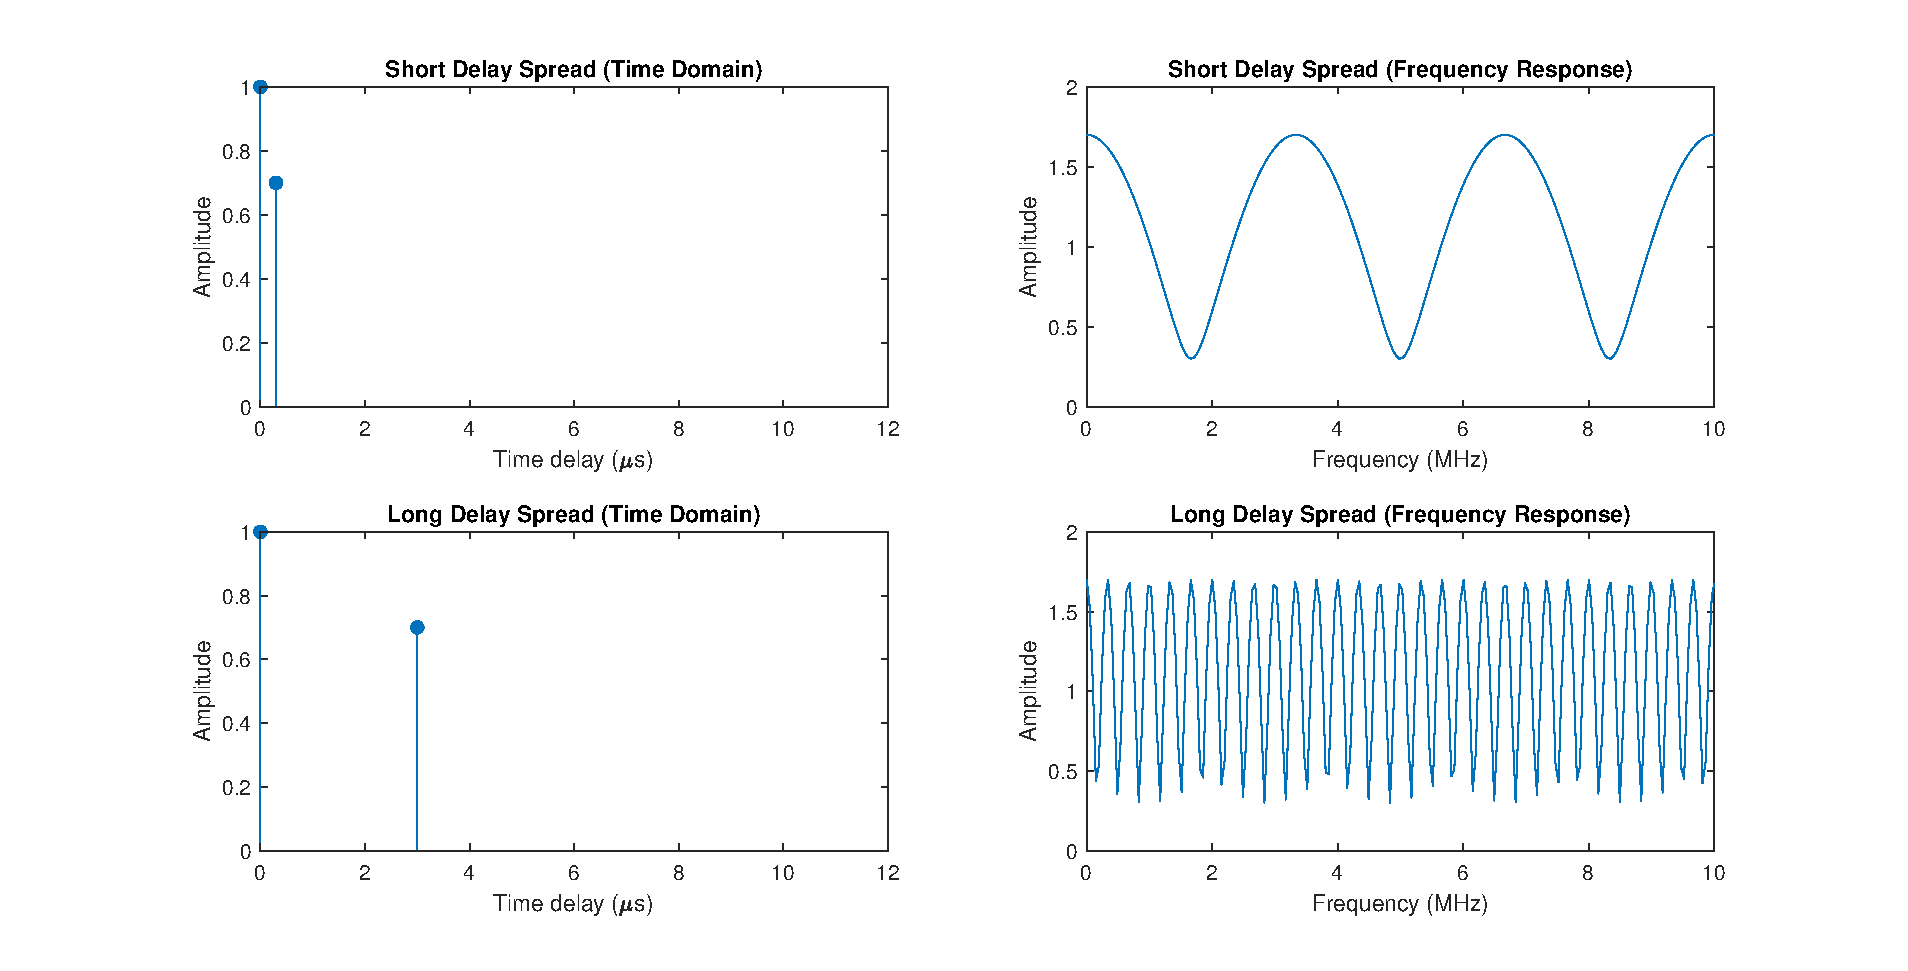
\includegraphics[width=1\textwidth]{delayspread1.eps}
    \end{figure}
\end{frame}
%----------------------------------------------------------------------------%
\begin{frame}
    \frametitle{Multipath propagation (8/8)}
    \begin{itemize}
        \item Two paths, each with an amplitude equal to 1.
    \end{itemize}
    \begin{figure}
        \centering
        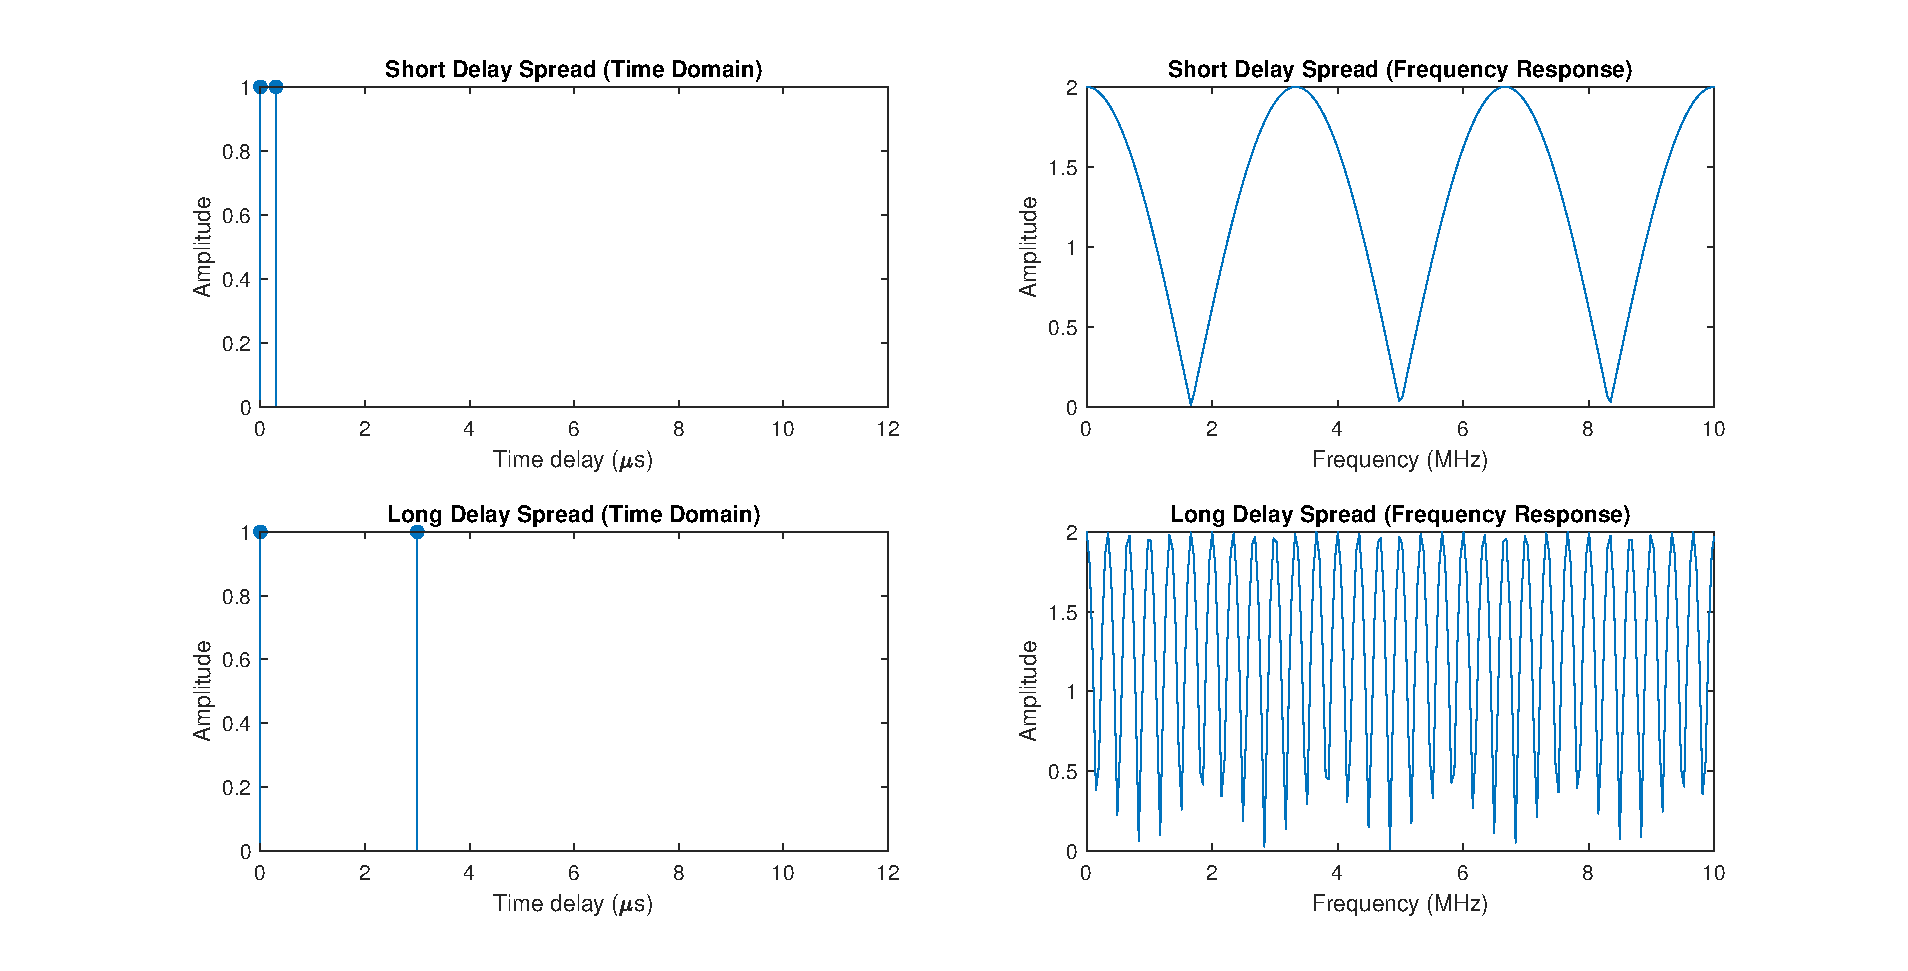
\includegraphics[width=1\textwidth]{delayspread2.eps}
    \end{figure}
\end{frame}
%----------------------------------------------------------------------------%


\begin{frame}
    \frametitle{Orthogonality (1/17)}
    \begin{itemize}
        \item Consider a set of transmitted carriers as follows:
        \begin{equation}
            \psi_{n}(t)=e^{j2\pi(f_{0}+\frac{n}{N\Delta t})t}
            \, \text{ for }\, n=0,1,...,N-1\,\text{ and }\,\Delta f=\frac{1}{N\Delta t}.
        \end{equation}
        \item $f_0$ : frequency of the 0-th subcarrier.
    \end{itemize}
    \begin{itemize}
        \item  We now show that every two carriers are orthogonal to each other. (proof is in next page)
        \begin{itemize}
            \item In summary:
             \begin{align}
                 \int_{a}^{b} \psi_{p}(t) \psi_{q}^\ast(t)dt=
                 \left \{
                 \begin{array}
                 {lr}(b-a)\,\text{ for }\, p=q\\
                 0\,\text{ for }\,p\neq q \,\text{ and }\,(b-a)=N\Delta t
                 \end{array}
                 \right.
            \end{align}
        \end{itemize}
    \end{itemize}
\end{frame}
%-----------------------------------------------------------------------------%
\begin{frame}
    \frametitle{Orthogonality (2/17)}
    \begin{itemize}
        \item Let $T = N\Delta t$ be the symbol duration, assuming the $p$-th and $q$-th subcarriers have frequencies $f_p = f_0 + p\Delta f$ and $f_q = f_0 + q\Delta f$.
        \item The integration is:
        \begin{align*}
            \int_0^{T} \psi_p(t)\psi_q^*(t)dt &= \int_0^{T} e^{j2\pi(p-q)\Delta f t} dt \\
            &= \frac{e^{j2\pi(p-q)\Delta f T} - 1}{j2\pi(p-q)\Delta f}
        \end{align*}
        \item For orthogonality:
        \begin{equation*}
            (p-q)\Delta f T = k \quad (k \in \mathbb{Z}, k \neq 0)
        \end{equation*}
        \item To find the minimum spacing for adjacent subcarriers ($|p-q|=1$), we set $k = 1$:
        \begin{equation*}
            \Delta f = \frac{1}{T} = \frac{1}{N\Delta t}
        \end{equation*}
    \end{itemize}
\end{frame}
%-----------------------------------------------------------------------------%
\begin{frame}
    \frametitle{Orthogonality (3/17)}
    \begin{itemize}
        \item The generalized condition for subcarrier spacing is:
    \end{itemize}
    
    \begin{center}
        $\Delta f = \frac{k}{N\Delta t} \quad (k \in \mathbb{Z}, k \neq 0)$ \\
        \vspace{0.2cm}
    \end{center}
    
    \begin{figure}
        \centering
        \setlength{\tabcolsep}{5pt} % 控制兩張圖之間的距離，讓它們靠近一點
        \begin{tabular}{cc}
            % 縮小寬度比例至 0.42，讓兩張圖在畫面上更集中、更靠近
            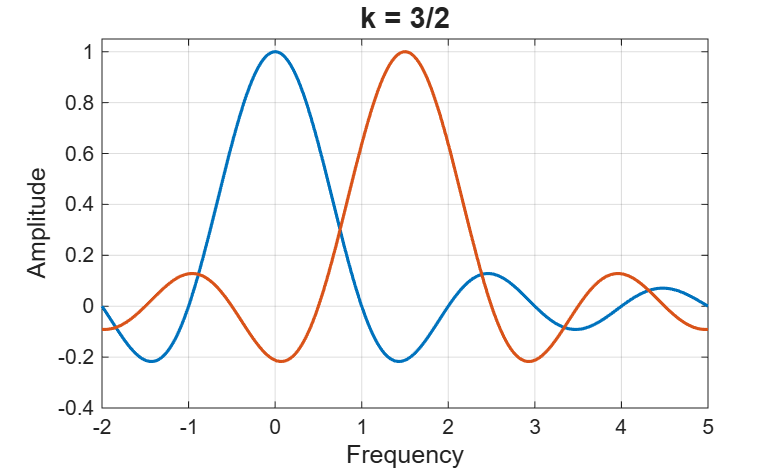
\includegraphics[width=0.45\textwidth]{k_15_freq.png} &
            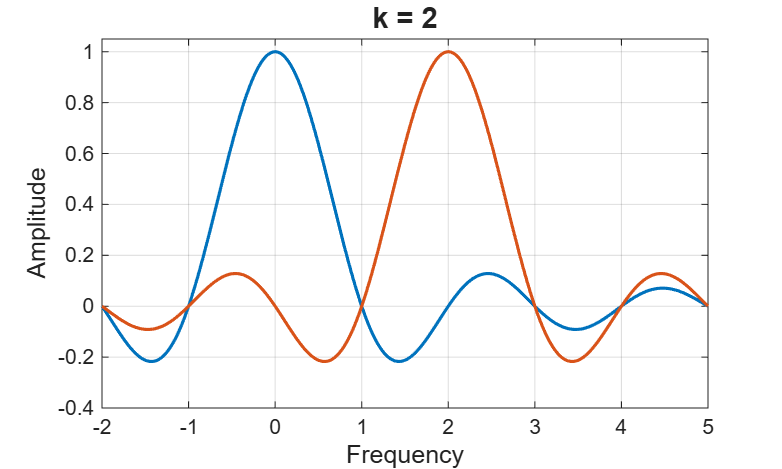
\includegraphics[width=0.45\textwidth]{k_20_freq.png} 
        \end{tabular}
    \end{figure}
    
    \vspace{0.3cm} % 在最下方強制留出空白
\end{frame}
%-----------------------------------------------------------------------------%
\begin{frame}
    \frametitle{Orthogonality (4/17)}
    \begin{itemize}
        \item Transmitted signal can be modeled as a rectangular pulse of length $N\Delta t$:
    \end{itemize}
    \vspace{0.3cm}
    \begin{center}
       {\Large
        $\text{rect}\left(\frac{t}{N\Delta t}\right) \xleftrightarrow{\mathcal{F}} N\Delta t \cdot \text{sinc}(f \cdot N\Delta t)$
        } 
        \vspace{0.6cm} % 拉開數學式與下面圖片的距離
        
        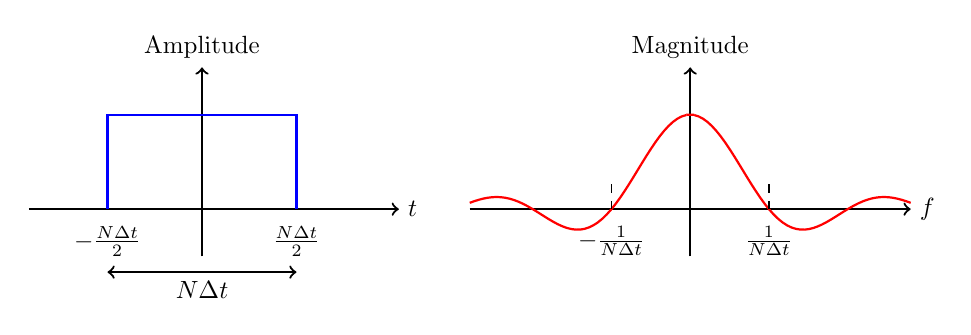
\begin{tikzpicture}[scale=1.0, thick, every node/.style={scale=0.9}]
            % --- Time Domain ---
            \begin{scope}[xshift=-3.1cm]
                \draw[->] (-2.2, 0) -- (2.5, 0) node[right] {$t$};
                \draw[->] (0, -0.6) -- (0, 1.8) node[above] {Amplitude};
                
                % 方波以 0 為中心，左右對稱
                \draw[blue, thick] (-1.2, 0) -- (-1.2, 1.2) -- (1.2, 1.2) -- (1.2, 0);
                
                \node[below] at (-1.2, -0.1) {$-\frac{N\Delta t}{2}$};
                \node[below] at (1.2, -0.1) {$\frac{N\Delta t}{2}$};
                
                % 標示總長度 N\Delta t (置於方波正下方)
                \draw[<->] (-1.2, -0.8) -- (1.2, -0.8) node[midway, below] {$N\Delta t$};
            \end{scope}

            % --- Frequency Domain ---
            \begin{scope}[xshift=3.1cm]
                \draw[->] (-2.8, 0) -- (2.8, 0) node[right] {$f$};
                \draw[->] (0, -0.6) -- (0, 1.8) node[above] {Magnitude};
                
                % 繪製 sinc 函數
                \draw[red, thick, domain=-2.8:-0.05, samples=50] plot (\x, {1.2*sin(\x*180)/(3.1415*\x)});
                \draw[red, thick, domain=0.05:2.8, samples=50] plot (\x, {1.2*sin(\x*180)/(3.1415*\x)});
                \draw[red, thick] (-0.05, 1.198) -- (0, 1.2) -- (0.05, 1.198); % Peak
                
                % 標示零點與向上的虛線
                \draw[dashed, semithick] (1, 0) -- (1, 0.4);
                \node[below] at (1, -0.1) {$\frac{1}{N\Delta t}$};
                
                \draw[dashed, semithick] (-1, 0) -- (-1, 0.4);
                \node[below] at (-1, -0.1) {$-\frac{1}{N\Delta t}$};
            \end{scope}
        \end{tikzpicture}
    \end{center}
\end{frame}
%-----------------------------------------------------------------------------%
\begin{frame}
    \frametitle{Orthogonality (5/17) --- Proof}
    \begin{itemize}
        \item $p=q$
        \begin{align*}
            &\int_{a}^{b} \psi_{p}(t) \psi_{p}^\ast(t)dt\\
            =&\int_{a}^{b} e^{j2\pi(f_{0}+\frac{p}{N\Delta t})t}e^{-j2\pi(f_{0}+\frac{p}{N\Delta t})t}dt\\
            =&\int_{a}^{b}e^{0}dt\\
            =&\int_{a}^{b}1dt\\
            =&b-a
        \end{align*}
    \end{itemize}
\end{frame}
%-----------------------------------------------------------------------------%
\begin{frame}
    \frametitle{Orthogonality (6/17) --- Proof}
    \begin{itemize}
        \item For the $p$-th subcarrier, the correlation coefficient over the interval $[a, b]$ is defined as:
        \begin{equation*}
            \rho = \frac{\int_a^b \psi_p(t)\psi_p^*(t)dt}{\sqrt{\int_a^b |\psi_p(t)|^2 dt \int_a^b |\psi_p^*(t)|^2 dt}}
        \end{equation*}
        \item The denominator becomes $\sqrt{(b-a) \cdot (b-a)} = b - a$.
        \item Thus, the correlation coefficient is exactly:
        \begin{equation*}
            \rho = \frac{b - a}{b - a} = 1
        \end{equation*}
    \end{itemize}
\end{frame}
%-----------------------------------------------------------------------------%
\begin{frame}
    \frametitle{Orthogonality (7/17) --- Proof}
    \begin{itemize}
        \item $p=q$, which $\psi_{q}(t)$ delay c
        \begin{align*}
            &\int_{a}^{b} \psi_{p}(t) \psi_{p}^\ast(t-c)dt\\
            &=\int_{a}^{b} e^{j2\pi(f_{0}+\frac{p}{N\Delta t})t}e^{-j2\pi(f_{0}+\frac{p}{N\Delta t})(t-c)}dt\\
            &=\int_{a}^{b} e^{j2\pi(f_{0}+\frac{p}{N\Delta t})c}dt\\
            &\text {let ${e^{j2\pi(f_{0}+\frac{p}{N\Delta t})c} = C}$ be a constant}\\
            &=C\int_ { a } ^ { b } 1 d t\\                                      
            &=C( b - a )                                                  
        \end{align*}
    \end{itemize}
\end{frame}
%-----------------------------------------------------------------------------%
\begin{frame}
    \frametitle{Orthogonality (8/17)--- Proof}
    \begin{itemize}
        \item The fundamental relationship is:
        \begin{equation*}
            \text{Energy} = \text{Power} \times \text{Time}
        \end{equation*}
        \item Here, the observation time is $(b-a)$.
        \item Therefore, the power of the signal is the constant $\mathbf{C}$.
    \end{itemize}
\end{frame}
%-----------------------------------------------------------------------------%
\begin{frame}
    \frametitle{Orthogonality (9/17) --- Proof}
    \begin{itemize}
        \item $p\neq q$ and $(b-a)=N\Delta t$
        \begin{align*}
           &\int_{a}^{b} \psi_{p}(t) \psi_{q}^\ast(t)dt\\
           =&\int_a^b e^{j2\pi(f_0 + \frac{p}{N\Delta t})t} \cdot e^{-j2\pi(f_0 + \frac{q}{N\Delta t})t}dt\\
           =&\int_a^b e^{j2\pi(\frac{p - q}{N\Delta t})t}dt \\
           =& \frac{e^{j2\pi(p-q) \frac{b}{N\Delta t}}-e^{j2\pi(p-q) \frac{a}{N\Delta t}}}{\frac{j2\pi(p-q)}{N\Delta t} }\\
        \end{align*}
    \end{itemize}
\end{frame}
%-----------------------------------------------------------------------------%
\begin{frame}
    \frametitle{Orthogonality (10/17) --- Proof}
    \begin{itemize}
        \item Continued from previous page: 
        \begin{align*}
           =& \frac{1}{j2\pi \left( \frac{p-q}{N\Delta t} \right)} \left( e^{j2\pi \left( \frac{p-q}{N\Delta t} \right) a} \cdot (e^{j2\pi(p-q) \frac{1}{N\Delta t}(b-a)}-1) \right)\\
           &\text{b-a is an observation period}=N\Delta t\\
           &\text{ and }  p-q \text{ is an integer so } e^{j2\pi (p-q)}=1\\
           =& \frac{1}{j2\pi \left( \frac{p-q}{N\Delta t} \right)} \left( e^{j2\pi \left( \frac{p-q}{N\Delta t} \right) a} \cdot (1-1) \right)\\
           =&0
        \end{align*}
    \end{itemize}
\end{frame}
%-----------------------------------------------------------------------------%
\begin{frame}
    \frametitle{Orthogonality (11/17) --- Proof}
    \begin{itemize}
        \item $p\neq q$ and $(b-a)=N\Delta t$, which $\psi_{p}(t)$ delay c and $\psi_{q}(t)$ delay d 
        \begin{align*}
           &\int_{a}^{b} \psi_{p}(t-c) \psi_{q}^\ast(t-d)dt\\
           =&\int_{a}^{b} e^{j2\pi(f_{0}+\frac{p}{N\Delta t})(t-c)}e^{-j2\pi(f_{0}+\frac{q}{N\Delta t})(t-d)}dt\\   
           =&\int_{a}^{b} e^{j2\pi f_{0}(t-c)}e^{j2\pi \frac{p}{N\Delta t}(t-c)}e^{-j2\pi f_{0}(t-d)}e^{-j2\pi \frac{q}{N\Delta t}(t-d)}dt\\   
           =&\int_{a}^{b} \frac{e^{j2\pi \frac{p}{N\Delta t}t}}{e^{j2\pi f_{0}c}e^{j2\pi \frac{p}{N\Delta t}c}}\frac{e^{-j2\pi \frac{q}{N\Delta t}t}}{e^{-j2\pi f_{0}d}e^{-j2\pi \frac{q}{N\Delta t}d}}dt\\
        \end{align*}
    \end{itemize}
\end{frame}
%-----------------------------------------------------------------------------%
\begin{frame}
    \frametitle{Orthogonality (12/17) --- Proof}
    \begin{itemize}
        \item Let ${e^{-j2\pi f_0c} e^{j2\pi f_0d} e^{-j2\pi(\frac{p}{N\Delta t})c} e^{j2\pi(\frac{q}{N\Delta t})d} = C}$ be a constant
    \end{itemize}
    \begin{align*}
        =&C\int_{a}^{b}e^{j2\pi(\frac{p}{N\Delta t})t}e^{-j2\pi(\frac{q}{N\Delta t})t}dt\\
        =&C\int_{a}^{b}e^{j2\pi\frac{(p-q)}{N\Delta t}t}dt \\
        =&C\frac{e^{j2\pi(p-q)\frac{b}{N\Delta t}}-e^{j2\pi(p-q)\frac{a}{N\Delta t}}}{\frac{j2\pi(p-q)}{N\Delta t} }\\
        =&C\frac{e^{j2\pi(p-q) \frac{b}{N\Delta t}}(1-e^{j2\pi(p-q) \frac{1}{N\Delta t}(a-b)})}{\frac{j2\pi(p-q)}{N\Delta t} }\\
        =&0 \text{ for } p\neq q\text{, and }(b-a)=N\Delta t
    \end{align*}
\end{frame}
%-----------------------------------------------------------------------------%
\begin{frame}
    \frametitle{Orthogonality (13/17)}
    \begin{itemize}
        \item The orthogonality condition is
        \begin{align*}
            \int_{a}^{b} \psi_{p}(t) \psi_{q}^\ast(t)dt=
            \left \{
            \begin{array}{lr}(b-a)\,\text{ for }\, p=q\\
            0\,\text{ for }\,p\neq q \,\text{ and }\,(b-a)=N\Delta t
            \end{array}
            \right.
        \end{align*}
        \item Consider the received OFDM signal and correlate it with $\psi_{k}(t)$:
        \begin{align*}
            &\int_{a}^{b}  D(t) \psi_{k}^\ast(t)dt
            =\int_{a}^{b} {\Big\{\sum_{n=0}^{N-1} d(n) \psi_{n}(t)\Big\}} \psi_{k}^\ast(t)dt\\
            =&d(k) \int_{a}^{b} \psi_{k}(t) \psi_{k}^\ast(t)dt + \sum_{n=0,n\neq k}^{N-1} d(n) \Big\{ \int_{a}^{b} \psi_{n}(t) \psi_{k}^\ast(t) dt\Big\}\\
            =&d(k) N \Delta t + 0 = d(k) N \Delta t
        \end{align*}
        \item Therefore, the $k$-th symbol can be recovered independently.
    \end{itemize}
\end{frame}
%-----------------------------------------------------------------------------%
\begin{frame}
    \frametitle{Orthogonality (14/17)}
    \begin{itemize}
        \item Consider one OFDM symbol over the interval \([a,b]\).The Fourier transform is given by:
        \begin{align*}
            \mathcal{X}(f) = \mathcal{F}\{D(t)\} = \int_{-\infty }^{\infty} D(t)e^{-j2\pi ft}dt = \int_{a }^{b} D(t)e^{-j2\pi ft}dt
        \end{align*}
        \item The $k$-th symbol can be recovered by sampling the spectrum at the $k$-th subcarrier frequency: 
        \begin{align*}
            &d(k) N \Delta t = \int_{a}^{b}  D(t) \psi_{k}^\ast(t)dt \\
            &=\int_{a}^{b}  D(t) e^{-j2\pi (f_0+k\Delta f)t}dt =\mathcal{X}(f_0+k\Delta f)
        \end{align*}
    \end{itemize}
\end{frame}
%-----------------------------------------------------------------------------%
\begin{frame}
    \frametitle{Orthogonality (15/17)}
    \begin{itemize}
        \item Transmitted Signal
    \end{itemize}
    \begin{figure}
        \centering
        %\hspace{-1cm}
        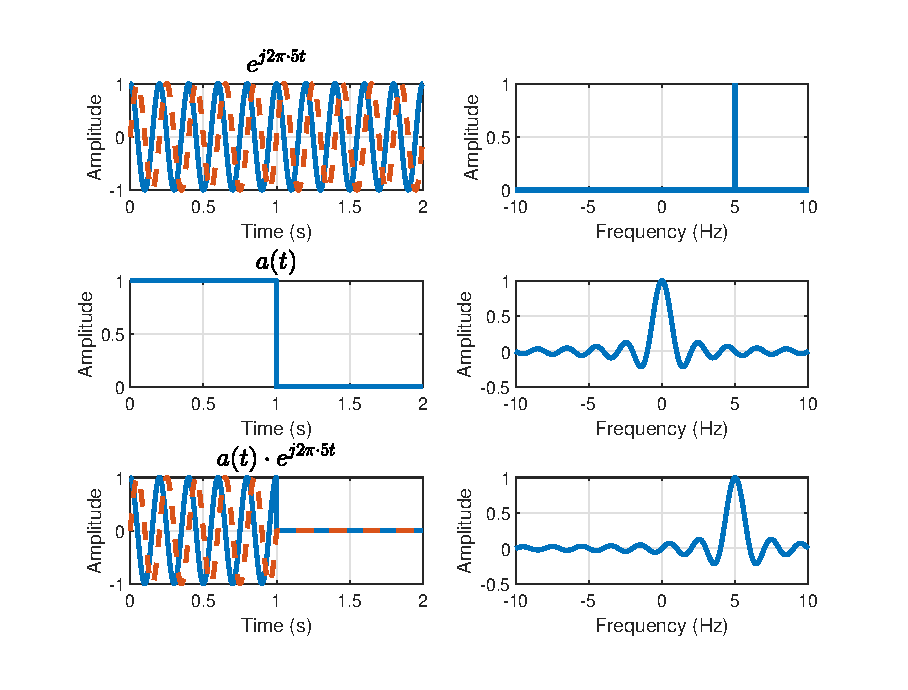
\includegraphics[width=0.8\textwidth, trim=0.5cm 0.5cm 0.5cm 0.5cm, clip]{transmitted_signal_v5.eps}
    \end{figure}
\end{frame}
%-----------------------------------------------------------------------------%
\begin{frame}
    \frametitle{Orthogonality (16/17)}
    \begin{itemize}
        \item Transmitted Signal in time domain
    \end{itemize}
    \begin{figure}
        \centering
        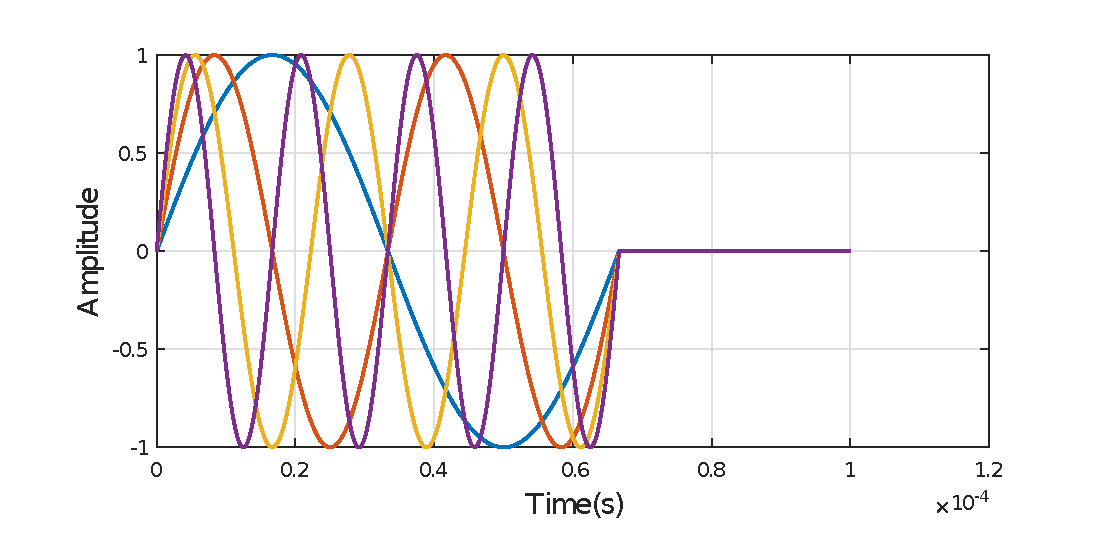
\includegraphics[width=0.99\textwidth]{OFDM_TD.eps}
    \end{figure}  
\end{frame}
%-----------------------------------------------------------------------------%
\begin{frame}
    \frametitle{Orthogonality (17/17)}
    \begin{itemize}
        \item Transmitted Signal in frequency domain
    \end{itemize}
    \begin{figure}
        \centering
        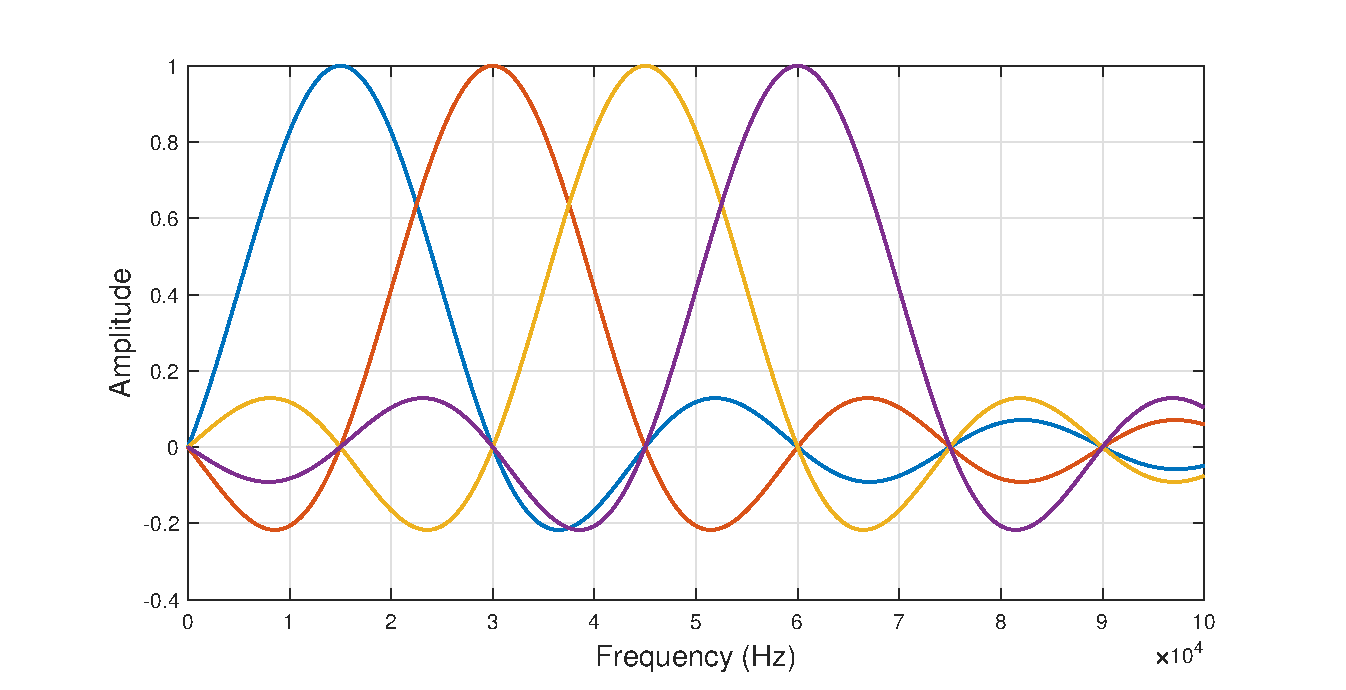
\includegraphics[width=0.97\textwidth]{OFDM_FD.eps}
    \end{figure} 
\end{frame}
%-----------------------------------------------------------------------------%
\begin{frame}
    \frametitle{Frequency Error Result in Inter-Carrier Interference (ICI) (1/2)}
    \begin{figure}
        \centering
        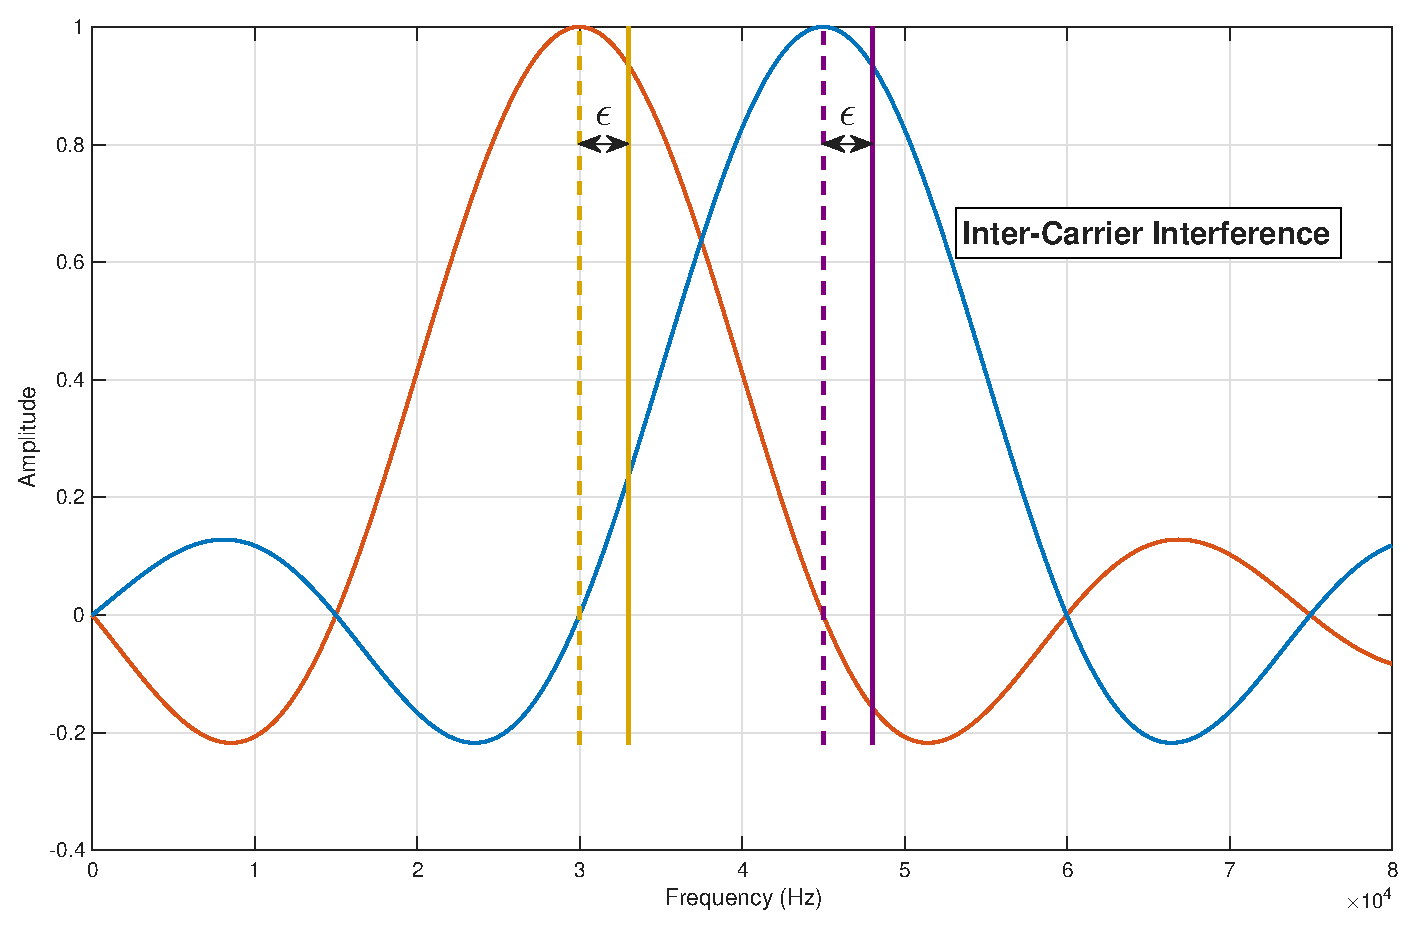
\includegraphics[width=0.8\textwidth]{frequency_error_ICI.eps}
    \end{figure}  
\end{frame}
%-----------------------------------------------------------------------------%
\begin{frame}
    \frametitle{Frequency Error Result in Inter-Carrier Interference (ICI) (2/2)}
    \begin{itemize}
        \item There are a few possible causes of frequency errors:
        \begin{itemize}
            \item Local Oscillator Mismatch of TX/RX
            \item Doppler Frequency Shift
            \item ADC/DAC Clock Mismatch
            \item Local Oscillator Short-term Instability
        \end{itemize}
    \end{itemize}
\end{frame}
%-----------------------------------------------------------------------------%
\begin{frame}
    \frametitle{Timing Synchronization Error Results in Inter-Symbol Interference (ISI) (1/4)}
    \begin{figure}
        \centering
        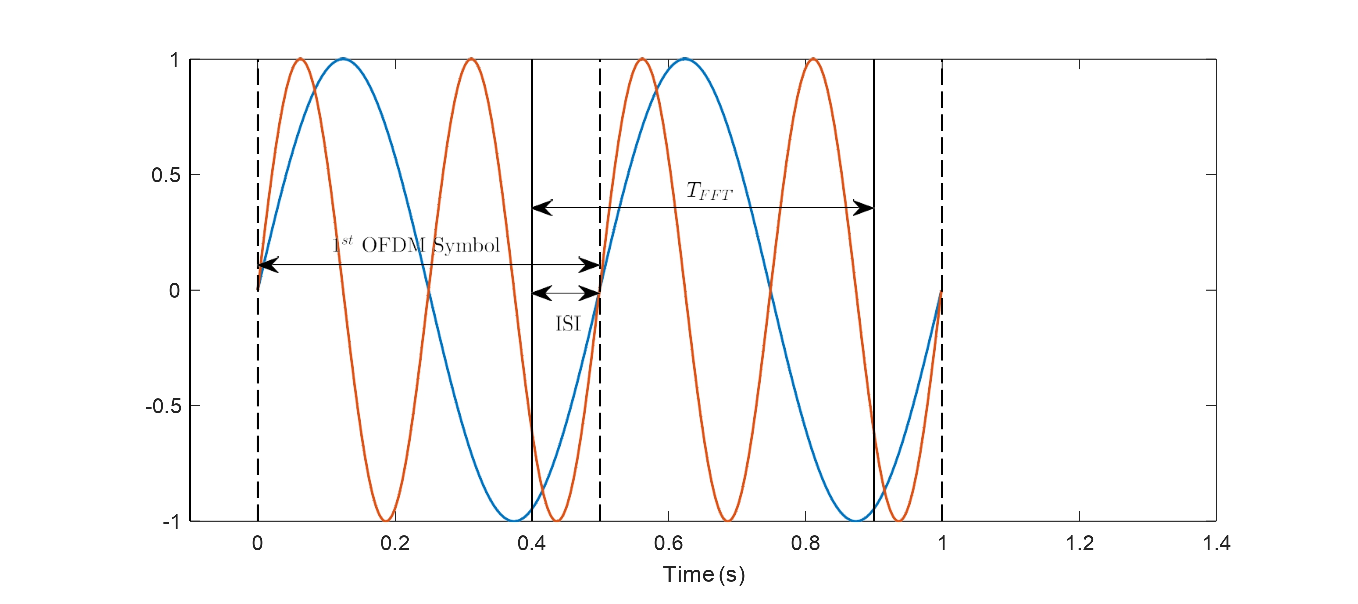
\includegraphics[width=0.8\textwidth]{Timing_Synchronization_Error_ISI.eps}
    \end{figure}
\end{frame}
%-----------------------------------------------------------------------------%
\begin{frame}
    \frametitle{Timing Synchronization Error Results in Inter-Symbol Interference (ISI) (2/4)}
\begin{itemize}
  \item Proof:
  \begin{itemize}
    \item In the demodulation window of FFT,
    \\{\scriptsize
    \[x(t)=\begin{cases}
    X_{1,\text{prev}}e^{j2\pi f_{1}t}\ +\ X_{2,\text{prev}}e^{j2\pi f_{2}t},&0.4\le t<0.5\\
    X_{1,\text{curr}}e^{j2\pi f_{1}(t-0.5)}\ +\ X_{2,\text{curr}}e^{j2\pi f_{2}(t-0.5)},&0.5\le t<0.9
    \end{cases}\]}
    \item $X_{m,\text{prev}}$ means the previous symbol of the $m$-th subcarrier, and $X_{m,\text{curr}}$ means the current symbol of the $m$-th subcarrier.
    \item Number of sampling points=N, $T_s=\frac{0.5}{N}s$, $t_s=0.4+nT_s$, $f_{1}=2$Hz, $f_{2}=4$Hz
    \\{\scriptsize
    \[x[n]=\begin{cases}
    X_{1,\text{prev}}e^{j2\pi f_{1}(0.4+nT_{s})}\ +\ X_{2,\text{prev}}e^{j2\pi f_{2}(0.4+nT_{s})},&0\le n<0.2N\\
    X_{1,\text{curr}}e^{j2\pi f_{1}(-0.1+nT_{s})}\ +\ X_{2,\text{curr}}e^{j2\pi f_{2}(-0.1+nT_{s})},&0.2N\le n<N
    \end{cases}\]}
  \end{itemize}
\end{itemize}
\end{frame}
%-----------------------------------------------------------------------------%
\begin{frame}
\frametitle{Timing Synchronization Error Results in Inter-Symbol Interference (ISI) (3/4)}
\begin{itemize}
  \item In the frequency domain,
  {\scriptsize
  \[
  \begin{aligned}
  Y[k]
  ={}&
  \frac{1}{N}
  \sum_{n=0}^{0.2N-1}
  \sum_{m=1}^{2}
  \left(
  X_{m,\text{prev}}
  e^{j2\pi f_m \cdot 0.4}
  e^{j2\pi\frac{m}{N}n}
  \right)
  e^{-j2\pi\frac{k}{N}n}
  \\[4pt]
  &+
  \frac{1}{N}
  \sum_{n=0.2N}^{N-1}
  \sum_{m=1}^{2}
  \left(
  X_{m,\text{curr}}
  e^{-j2\pi f_m \cdot 0.1}
  e^{j2\pi\frac{m}{N}n}
  \right)
  e^{-j2\pi\frac{k}{N}n}
  \\[4pt]
  ={}&
  \sum_{m=1}^{2}
  X_{m,\text{prev}}\alpha_{m\rightarrow k}
  +
  \sum_{m=1}^{2}
  X_{m,\text{curr}}\beta_{m\rightarrow k}.
  \end{aligned}
  \]
  }
\end{itemize}
\end{frame}
%-----------------------------------------------------------------------------%
\begin{frame}
\frametitle{Timing Synchronization Error Results in Inter-Symbol Interference (ISI) (4/4)}
\begin{itemize}
  \item When $m=k$,
  {\small
  \[
  \begin{aligned}
  \alpha_{k\rightarrow k}
  &=
  \frac{e^{j0.8\pi f_k}}{N}(0.2N)
  \\
  &=
  0.2e^{j0.8\pi f_k}
  \neq 0
  \qquad \text{(ISI)}
  \\[8pt]
  \beta_{k\rightarrow k}
  &=
  \frac{e^{-j0.2\pi f_k}}{N}
  \sum_{n=0.2N}^{N-1}1
  \\
  &=
  \frac{e^{-j0.2\pi f_k}}{N}(0.8N)
  \\
  &=
  0.8e^{-j0.2\pi f_k}
  \end{aligned}
  \]
  }
\end{itemize}
\end{frame}
%-----------------------------------------------------------------------------%
\begin{frame}
    \frametitle{Timing Synchronization Error Results in Inter-Carrier Interference (ICI) (1/8)}
    \begin{figure}
        \centering
        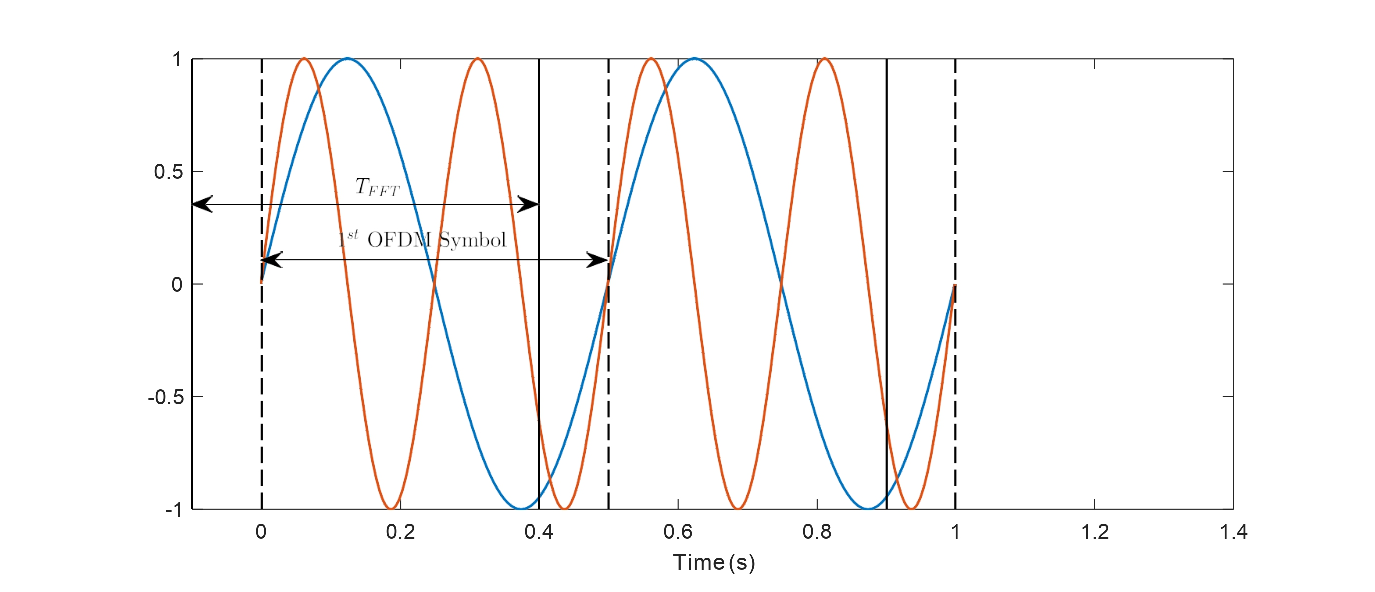
\includegraphics[width=0.8\textwidth]{Timing_Synchronization_Error_ICI.eps}
    \end{figure}
\end{frame}
%-----------------------------------------------------------------------------%
\begin{frame}
    \frametitle{Timing Synchronization Error Results in Inter-Carrier Interference (ICI) (2/8)}
    \begin{figure}
        \centering
        
\includegraphics[width=0.8\textwidth]{time_synchronization_error_ICI_2.eps}
    \end{figure}  
\end{frame}
%-----------------------------------------------------------------------------%
\begin{frame}
    \frametitle{Timing Synchronization Error Results in Inter-Carrier Interference (ICI) (3/8)}
\begin{itemize}
  \item Proof:
  \begin{itemize}
    \item In the demodulation window of FFT,
    \\{\scriptsize
    \[x(t)=\begin{cases}
    X_{1,\text{prev}}e^{j2\pi f_{1}(t+0.5)}\ +\ X_{2,\text{prev}}e^{j2\pi f_{2}(t+0.5)},&-0.1\le t<0\\
    X_{1,\text{curr}}e^{j2\pi f_{1}t}\ +\ X_{2,\text{curr}}e^{j2\pi f_{2}t},&0\le t<0.4
    \end{cases}\]}
    \item Number of sampling points=N, $T_s=\frac{0.5}{N}s$, $f_{1}=2$Hz, $f_{2}=4$Hz
    \\{\scriptsize
    \[x[n]=\begin{cases}
    X_{1,\text{prev}}e^{j2\pi f_{1}(nT_{s}+0.5)}\ +\ X_{2,\text{prev}}e^{j2\pi f_{2}(nT_{s}+0.5)},&-0.2N\le n<0\\
    X_{1,\text{curr}}e^{j2\pi f_{1}nT_{s}}\ +\ X_{2,\text{curr}}e^{j2\pi f_{2}nT_{s}},&0\le n<0.8N
    \end{cases}\]}
  \end{itemize}
\end{itemize}
\end{frame}
%-----------------------------------------------------------------------------%
\begin{frame}
\frametitle{Timing Synchronization Error Results in Inter-Carrier Interference (ICI) (4/8)}
\begin{itemize}
  \item In the frequency domain, 
  \begin{flalign*}
    &Y[k]&
    \\=&\frac{1}{N}\sum_{n=-0.2N}^{-1}\sum_{m=1}^{2}(X_{m,\text{prev}}e^{j2\pi f_{m}(-0.5) e^{j2\pi \frac{m}{N}n}})e^{-j2\pi \frac{k}{N}n}&
    \\+&\frac{1}{N}\sum_{n=0}^{0.8N-1}\sum_{m=1}^{2}(X_{m,\text{curr}}e^{j2\pi \frac{m}{N}n})e^{-j2\pi \frac{k}{N}n}&
    \\=&\sum_{m=1}^{2}X_{m,\text{prev}}\cdot \alpha_{m\rightarrow k}+\sum_{m=1}^{2}X_{m,\text{curr}}\cdot \beta_{m\rightarrow k}&
  \end{flalign*}
\end{itemize}
\end{frame}
%-----------------------------------------------------------------------------%
\begin{frame}
\frametitle{Timing Synchronization Error Results in Inter-Carrier Interference (ICI) (5/8)}
\begin{itemize}
  \item When $m=k$,
  \begin{flalign*}
    &\alpha_{k\rightarrow k} =\frac{e^{j\pi f_{k}}}{N}(0.2N)=0.2\cdot e^{j\pi f_{k}} \not= 0\ \ \text{(ISI)} &\\
    &\beta_{k\rightarrow k}=\frac{1}{N}\sum_{n=0}^{0.8N-1}1=\frac{0.8N}{N} =0.8&
  \end{flalign*}
\end{itemize}
\end{frame}
%-----------------------------------------------------------------------------%
\begin{frame}
\frametitle{Timing Synchronization Error Results in Inter-Carrier Interference (ICI) (6/8)}
\begin{itemize}
  \item When $m\not= k$, 
  \begin{flalign*}
    &\alpha_{m\rightarrow k}=\frac{e^{j\pi f_{m}}}{N}\frac{e^{\pm j2\pi (-0.2)-1}}{1-e^{\pm j2\pi \frac{1}{N}}}\not= 0\ \ \text{(ISI, ICI)}&\\
    &\beta_{m\rightarrow k}=\frac{1}{N}\frac{1-e^{\pm j2\pi (0.8)}}{1-e^{\pm j2\pi \frac{1}{N}}}\not= 0\ \ \text{(ICI)}&
  \end{flalign*}
\end{itemize}
\end{frame}
%-----------------------------------------------------------------------------%
\begin{frame}
\frametitle{Timing Synchronization Error Results in Inter-Carrier Interference (ICI) (7/8)}
\begin{itemize}
    \item Current subcarrier signals:\\
    \[\begin{cases}
    Y[1]=0.8X_{1,\text{curr}}+\beta_{2\rightarrow 1}X_{2,\text{curr}}+\alpha_{1\rightarrow 1}X_{1,\text{prev}}+\alpha_{2\rightarrow 1}X_{2,\text{prev}}\\
    Y[2]=0.8X_{2,\text{curr}}+\beta_{1\rightarrow 2}X_{1,\text{curr}}+\alpha_{2\rightarrow 2}X_{2,\text{prev}}+\alpha_{1\rightarrow 2}X_{1,\text{prev}}
    \end{cases}\]
    \item The subcarrier experiences energy loss and generates ICI.
    \item Also, the previous subcarrier signals will generate ISI and ICI to the current subcarrier signals.
\end{itemize}
\end{frame}
%-----------------------------------------------------------------------------%
\begin{frame}
\frametitle{Timing Synchronization Error Results in Inter-Carrier Interference (ICI) (8/8)}
\begin{itemize}
  \item If no timing synchronization error, $Y[k]=X_{k}^{curr}$
  \item Proof:
  \begin{itemize}
    \item When $m=k$,
    \\\[\beta_{k\rightarrow k}=\frac{1}{N}\sum_{n=0}^{N-1}1=\frac{N}{N}=1\]
    \item When $m\not= k$,
    \\\[\beta_{1\rightarrow 2}=\frac{1}{N}\frac{1-e^{-j2\pi (1)}}{1-e^{-j2\pi \frac{1}{N}}}= 0\]
    \\\[\beta_{2\rightarrow 1}=\frac{1}{N}\frac{1-e^{j2\pi (1)}}{1-e^{j2\pi \frac{1}{N}}}= 0\]
  \end{itemize}
\end{itemize}
\end{frame}
%-----------------------------------------------------------------------------%
\begin{frame}
    \frametitle{Mathematical Expression of OFDM Signal (1/4)}
    \begin{itemize}
        \item Frequency Division Multiplexing
    \end{itemize}
    \begin{figure}
        \centering
        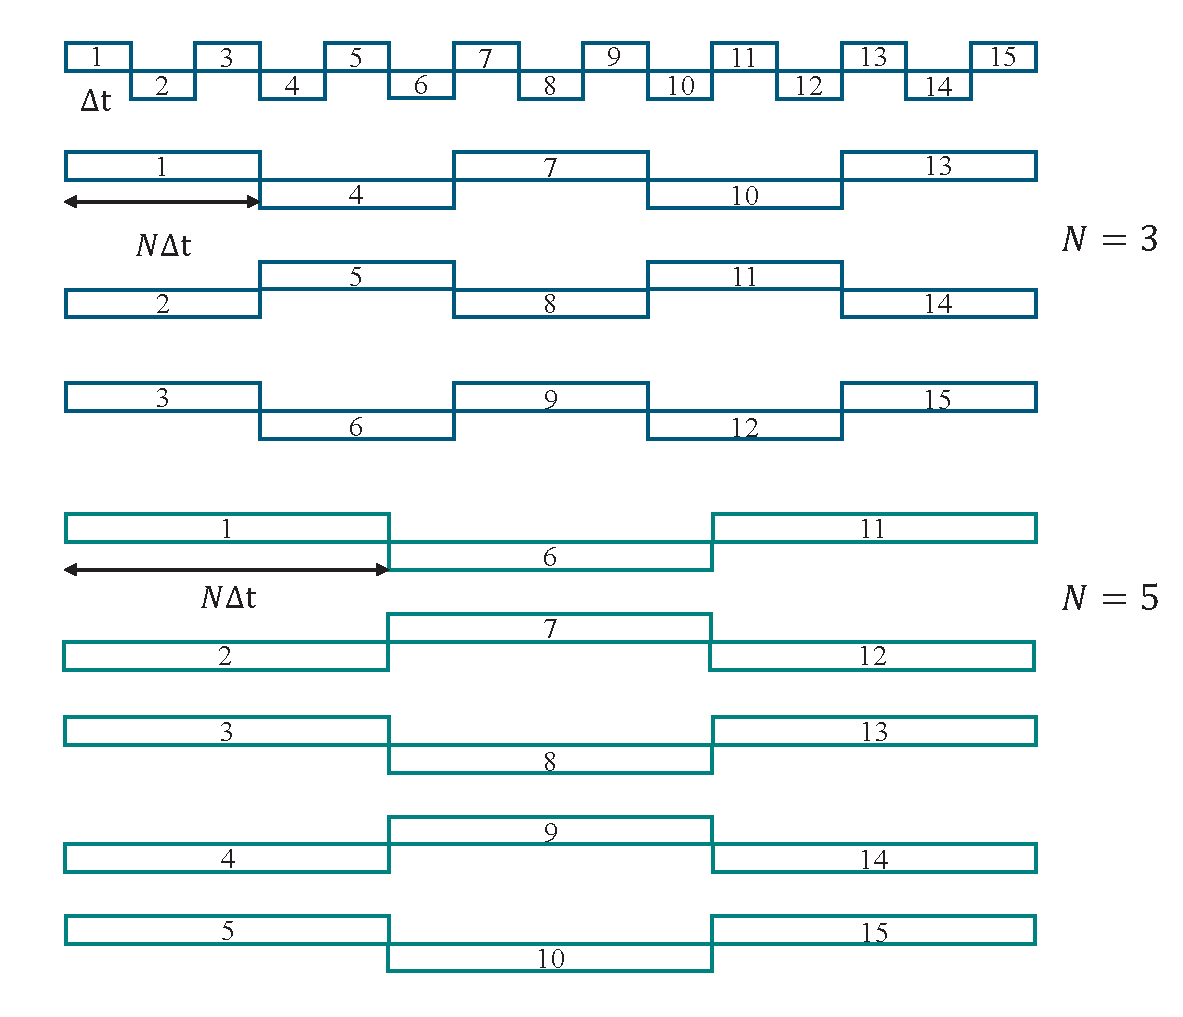
\includegraphics[width=0.6\textwidth]{FDM.eps}

    \end{figure}
\end{frame}
%-----------------------------------------------------------------------------%
\begin{frame}
    \frametitle{Mathematical Expression of OFDM Signal (2/4)}
    \begin{itemize}
        \item From above, we know that $\psi_{n}(t)$  is the orthogonal signal set. An OFDM signal based on this orthogonal signal set can be written as:
        \begin{equation} 
            x(t)=Re\Big\{\sum_{k=-\infty}^{\infty}\sum_{n=0}^{N-1}d_{k,n}\psi_{n}(t-kT)\Big\}
        \end{equation}
        \begin{align*} 
            \text{ where }\psi_{n}(t)&=e^{j2\pi f_{n}t}\,&\text{ for }\,n=0,1,...,N-1\\
            f_{n}&=f_{0}+\frac{n}{T},&T=N\Delta t\\
            d_{k,n}&=a_{k,n}+jb_{k,n}\\
        \end{align*}
        \item  $d_{k,n}$: transmitted data on the $n$-th carrier of the $k$-th symbol.
    \end{itemize}
\end{frame}
%-----------------------------------------------------------------------------%
\begin{frame}
    \frametitle{Mathematical Expression of OFDM Signal (3/4)}
    \begin{itemize}
        \item T : OFDM symbol duration
        \item  $d_{k,n}$: transmitted data on the $n$-th carrier of the $k$-th symbol.
        \begin{align}
            x(t)&=Re\Big\{\sum_{k=-\infty}^{\infty}\sum_{n=0}^{N-1}d_{k,n}\psi_{n}(t-kT)\Big\}\\
            &=\sum_{k=-\infty}^{\infty}\sum_{n=0}^{N-1}\Big\{a_{k,n}\cos{(2{\pi}f_{n}(t-kT))}-b_{k,n}\sin{(2{\pi}f_{n}(t-kT))}\Big\}\
        \end{align}
        \item If there is only one OFDM symbol ( i.e. $k$ = 0 ), it can be simplified as:
        \begin{equation} 
            x(t)=\sum_{n=0}^{N-1}\{a(n)\cos{(2{\pi}f_{n}t)}-b(n)\sin{(2{\pi}f_{n}t)}\}
        \end{equation}
    \end{itemize}
\end{frame}
%-----------------------------------------------------------------------------%
\begin{frame}
    \frametitle{Mathematical Expression of OFDM Signal (4/4)}
    \begin{itemize}
        \item Visualization of the mathematical expression (for $N = 5$)
    \end{itemize}
    \begin{figure}
        \centering
        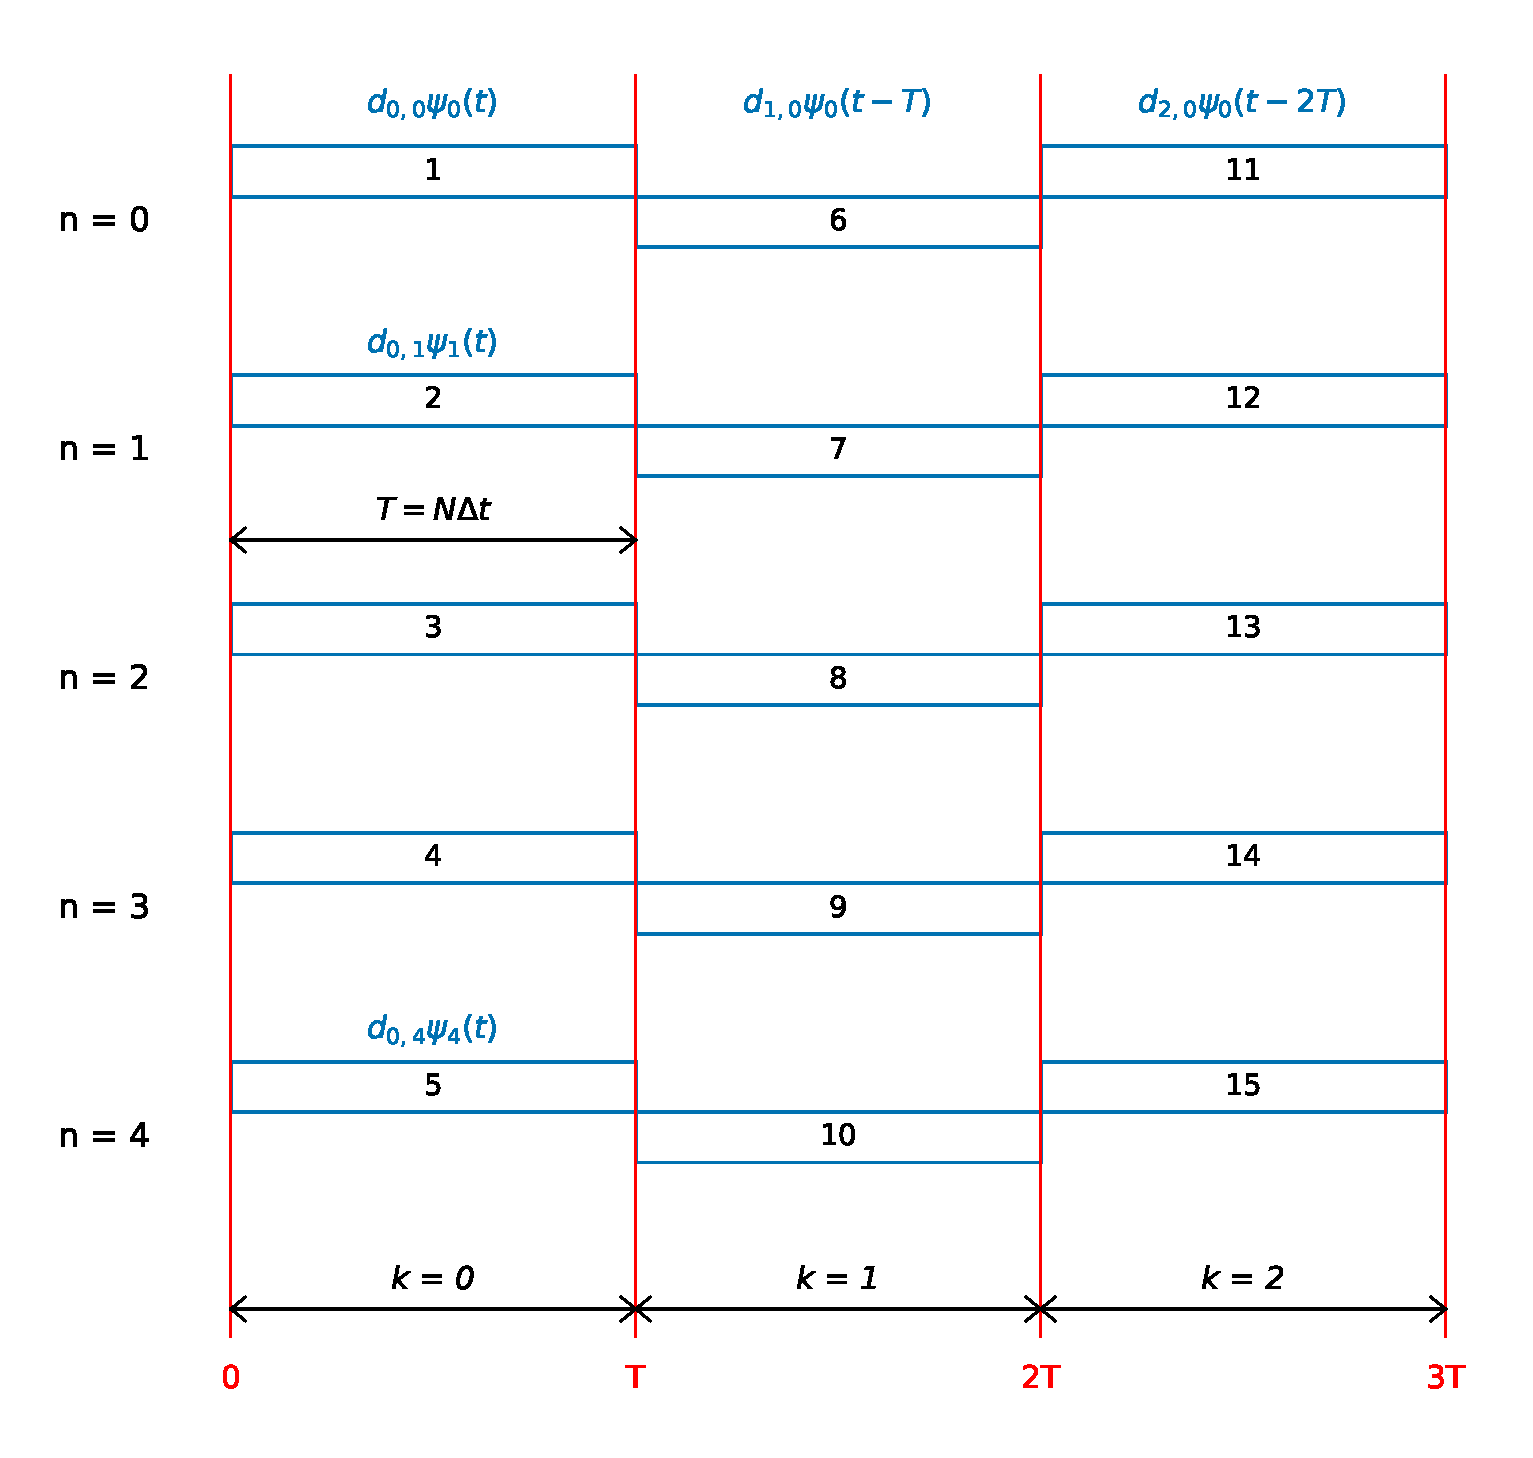
\includegraphics[width=0.6\textwidth]{FDM_final.eps}

    \end{figure}
\end{frame}
%-----------------------------------------------------------------------------%
\begin{frame}
    \frametitle{Multi-carrier Equivalent Implementation by using IDFT (1/6)}
    \begin{itemize}
        \item According to the structure of Tx, it must use $N$ oscillators. 
        \item That increases the hardware complexity.
        \item The equivalent method is using IDFT (IFFT).
    \end{itemize}
\end{frame}
%-----------------------------------------------------------------------------%
\begin{frame}
    \frametitle{Multi-carrier Equivalent Implementation by using IDFT (2/6)}
    \begin{itemize}
        \item In general, each carrier can be expressed as:
        \begin{equation}
            S_{c}(t)=A_{c}(t)e^{j(2\pi f_{c}t+\phi_{c}(t))}   
        \end{equation}
        \item We assume that there are \(N\) carriers in the OFDM signal.
        \item Then the total complex signal \(S_{s}(t)\) can be represented by:
        \begin{equation}
            S_{s}(t)=\frac{1}{N}\sum_{n=0}^{N-1}A_{n}(t)e^{j(2\pi f_{n}t+\phi_{n}(t))}
        \end{equation}
        \item where \( f_{n}=f_{0}+n\Delta f \) \\
        \item and \(A_{n}(t)\), \(\phi_{n}(t)\), \(f_{n}\) are the amplitude, phase, and carrier frequency of the \(n\)-th carrier, respectively.
    \end{itemize}
\end{frame}
%-----------------------------------------------------------------------------%
\begin{frame}
    \frametitle{Multi-carrier Equivalent Implementation by using IDFT (3/6)}
    \begin{itemize}
        \item  Then we sample the signal at a sampling frequency$\frac{1}{\Delta t}$ , and $A_{n}(t)$ and $\phi_{n}(t)$ becomes:
        \begin{align}
            \phi_{n}(t)&=\phi_{n}\\
            A_{n}(t)&=A_{n}\\
            S_{s}(k\Delta t)=\frac{1}{N}\sum_{n=0}^{N-1}&A_{n}e^{j(2\pi(f_{0}+n\Delta f)k\Delta t+\phi_{n})}
        \end{align}
    \end{itemize}
    \begin{itemize}
        \item Then the sampled signal can be expressed as:
        \begin{equation}
            S_{s}(k\Delta t)=(\frac{1}{N}\sum_{n=0}^{N-1}A_{n}e^{j\phi_{n}}e^{j2\pi nk\Delta f\Delta t})e^{j2\pi f_{0}k\Delta t}       
        \end{equation}
    \end{itemize}
\end{frame}
%-----------------------------------------------------------------------------%
\begin{frame}
    \frametitle{Multi-carrier Equivalent Implementation by using IDFT (4/6)}
    \begin{itemize}
        \item The inverse discrete Fourier transform (IDFT) is defined as the following:
        \begin{equation}
            f(k\Delta t)=\frac{1}{N}\sum_{n=0}^{N-1}F(n\Delta f)e^{j2\pi nk/N}
        \end{equation}
    \end{itemize}
    \begin{itemize}
        \item Comparing eq.(13) and eq.(14), the condition must be satisfied in order to make eq.(13) an inverse Fourier transform relationship:
        \begin{equation}
            \Delta f=\frac{1}{N\Delta t}
        \end{equation}
    \end{itemize}
\end{frame}
%-----------------------------------------------------------------------------%
\begin{frame}
    \frametitle{Multi-carrier Equivalent Implementation by using IDFT (5/6)}
    \begin{itemize}
        \item If eq.(15) is satisfied,
        \begin{itemize}
             \item $A_{n}e^{j\phi _{n}}$is the frequency domain signal.
             \item $S_{s}(k\Delta t)$is the time domain signal.
             \item $\Delta f$ is the sub-channel spacing.
             \item $N\Delta t$ is the symbol duration in each sub-channel.
        \end{itemize}
    \end{itemize}
    \begin{itemize}
        \item This outcome is the same as the result obtained in the system of Figure 1. Therefore IDFT can be used to generate an OFDM transmission signal.
    \end{itemize}
\end{frame}
%-----------------------------------------------------------------------------%
\begin{frame}
    \frametitle{Multi-carrier Equivalent Implementation by using IDFT (6/6)}
        \centering
        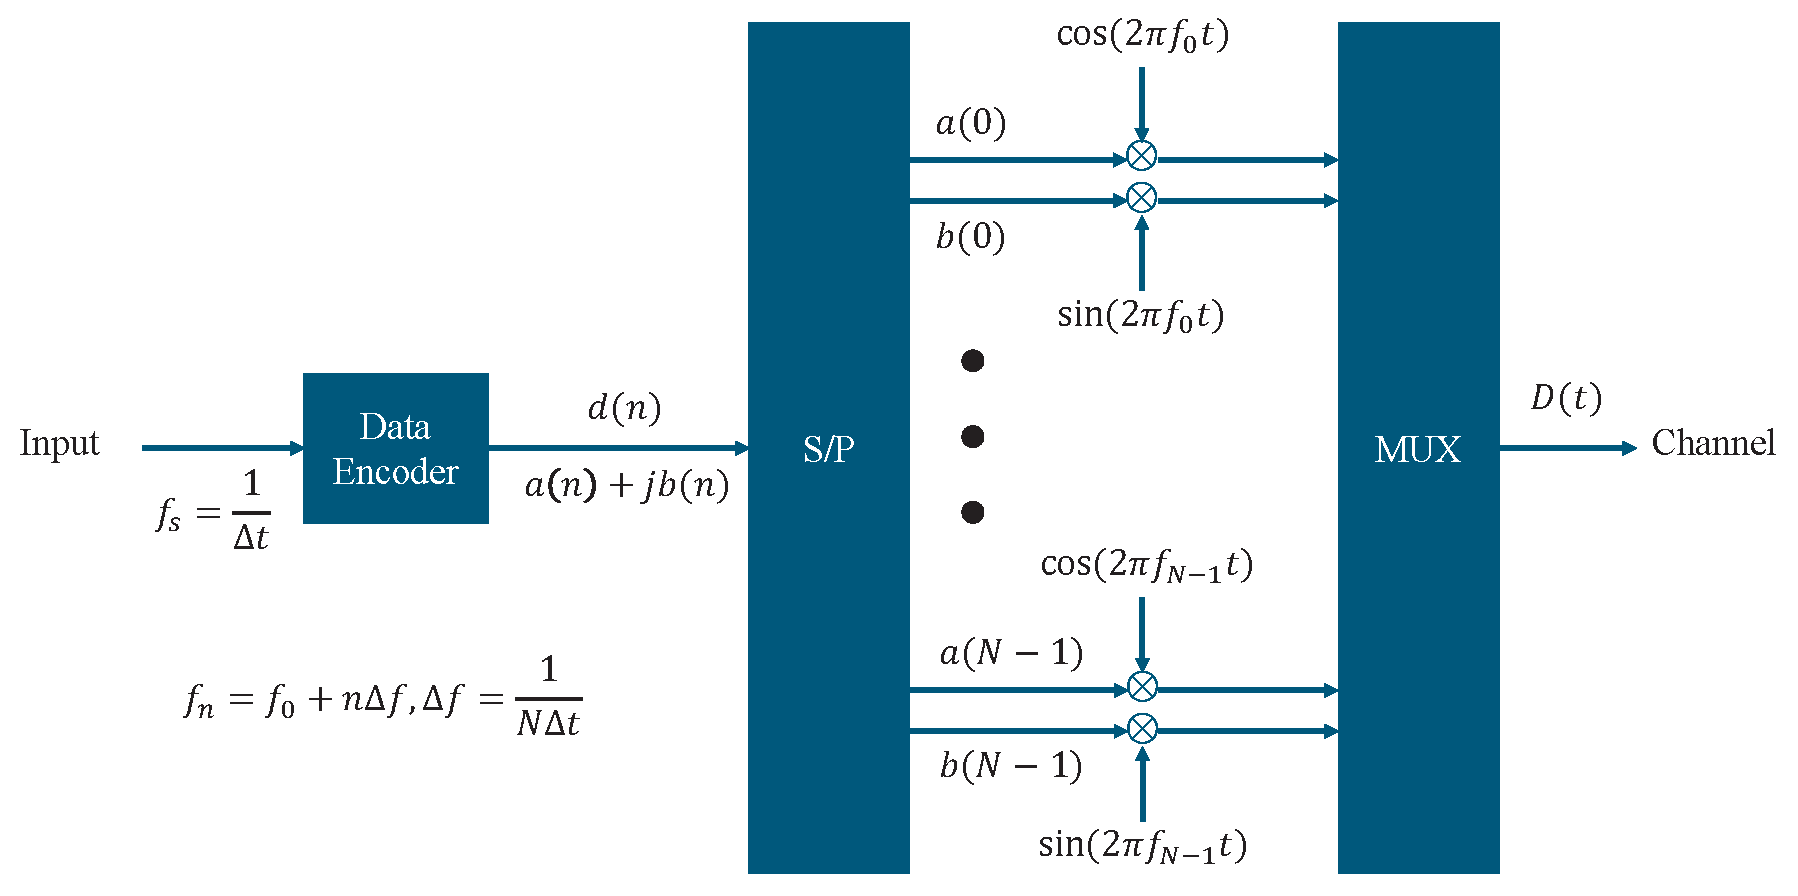
\includegraphics[width=0.6\textwidth]{Multi_carrier_Equivalent_1.eps}
        \vspace{5mm}
        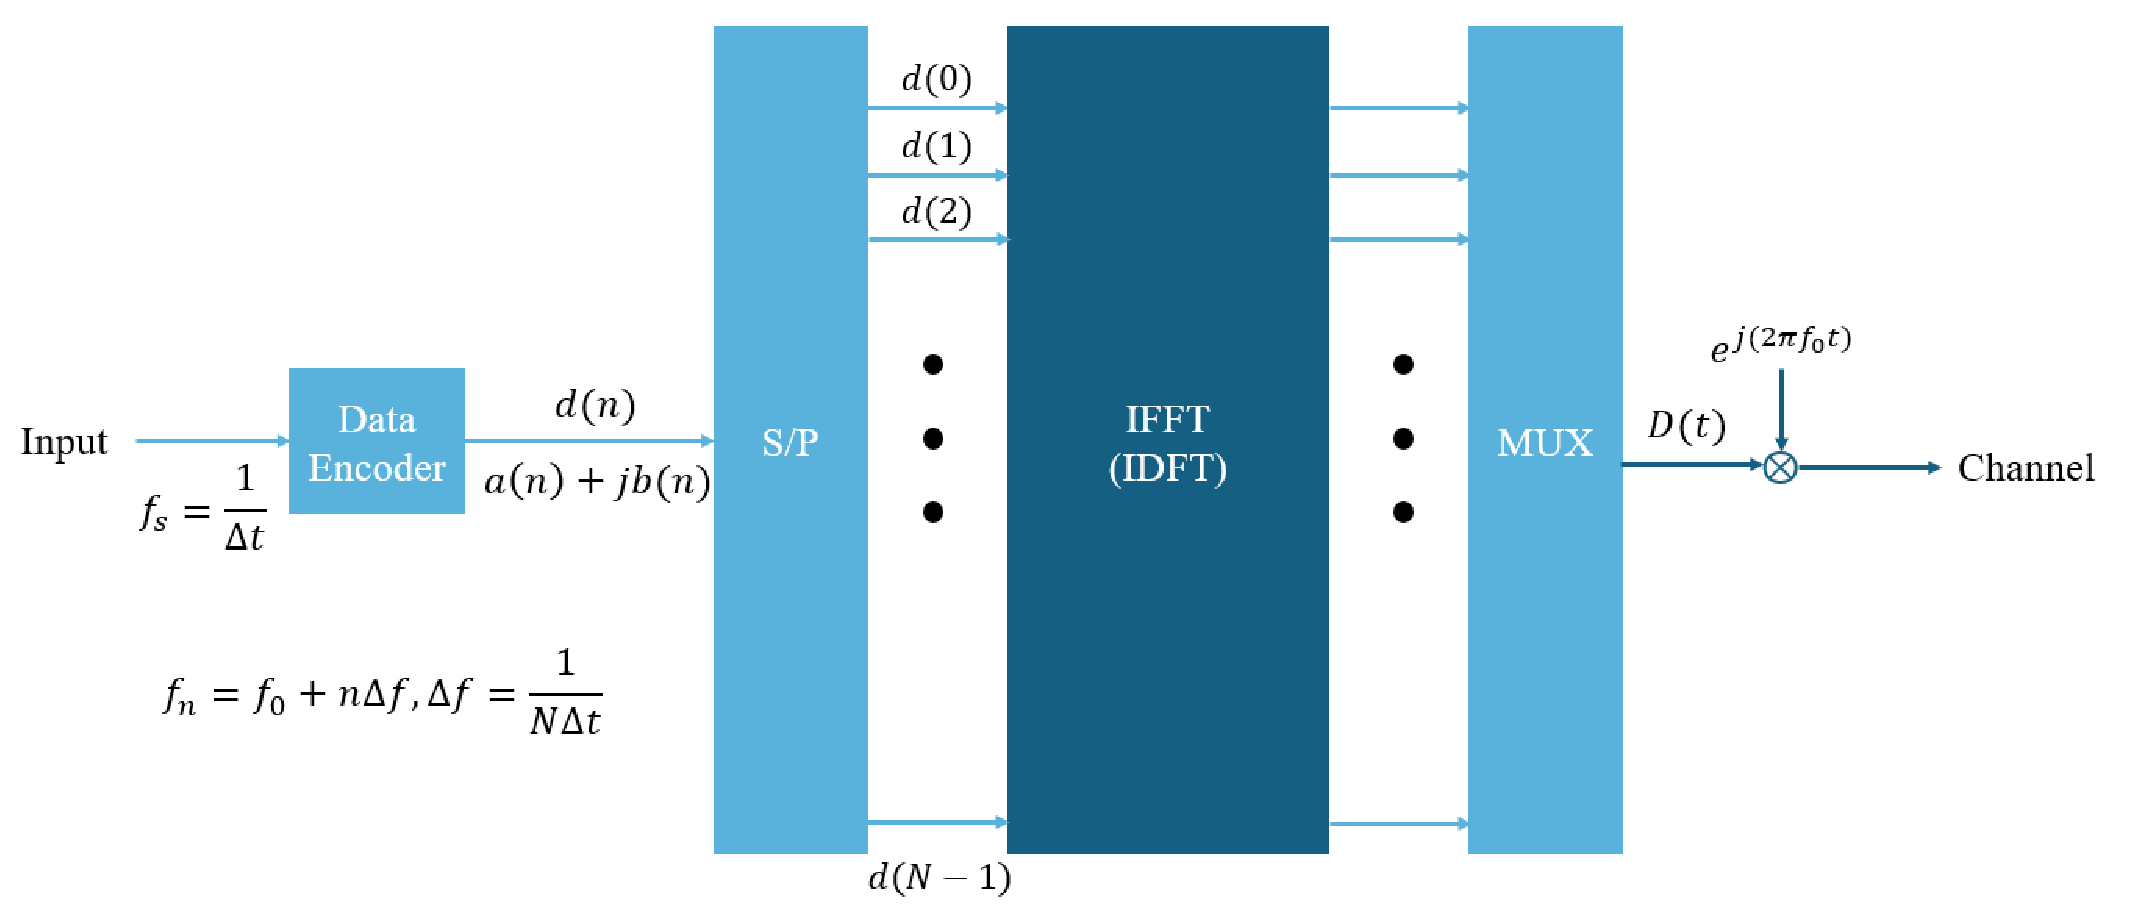
\includegraphics[width=0.6\textwidth]{Multi_carrier_Equivalent_2.eps}
\end{frame}
%-----------------------------------------------------------------------------%
\begin{frame}
    \frametitle{Cyclic Prefix(1/13)}
    \begin{itemize}
        \item In  multipath channel, delayed replicas of previous OFDM signal lead to ISI between successive OFDM signals.
    \end{itemize}
    \begin{figure}
        \centering
        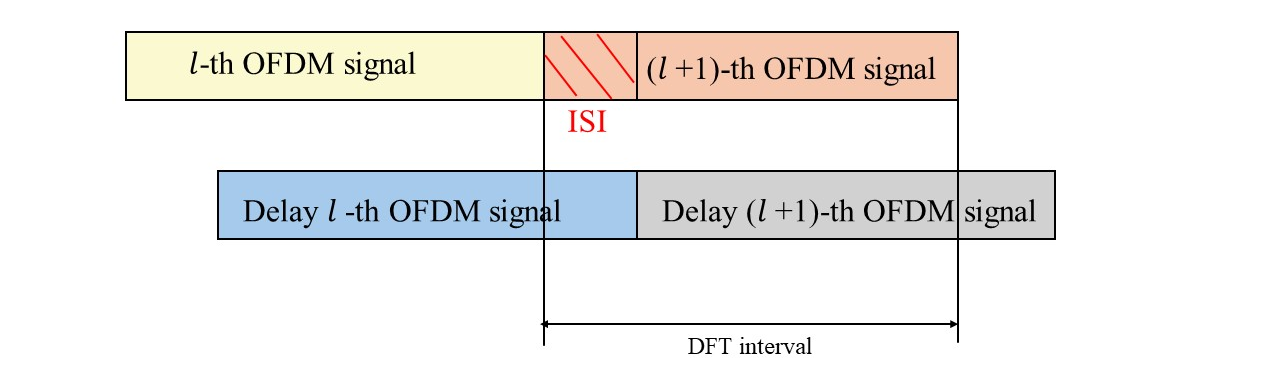
\includegraphics[width=0.7\textwidth]{CP_1.png}
    \end{figure}
    \begin{itemize}
        \item Solution : Insert a guard interval (GI) between successive OFDM signals.
    \end{itemize}
    \begin{figure}
        \centering
        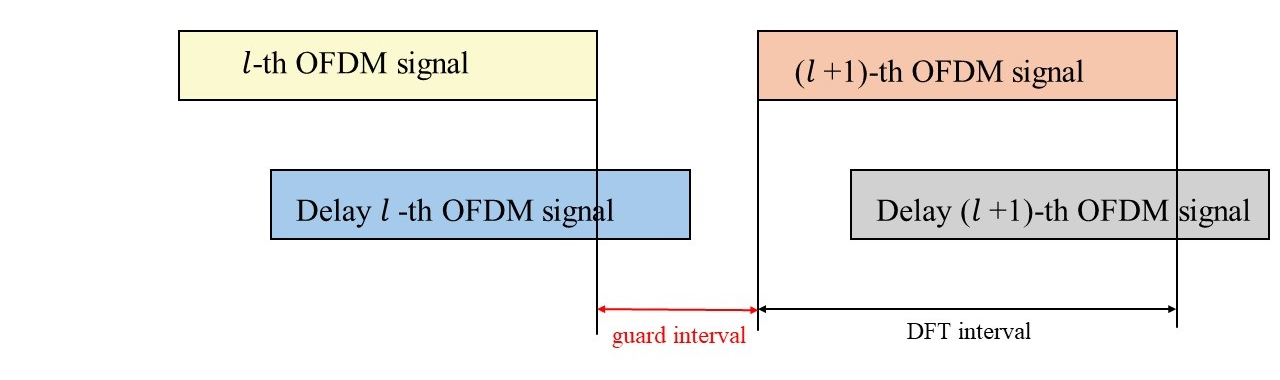
\includegraphics[width=0.7\textwidth]{CP_2.png}
    \end{figure}
\end{frame}
%-----------------------------------------------------------------------------%
\begin{frame}
    \frametitle{Cyclic Prefix(2/13)}
    \begin{itemize}
        \item However, adding guard interval breaks the orthogonality, leading to intercarrier interference (ICI).
    \end{itemize}
    \begin{figure}
        \centering
        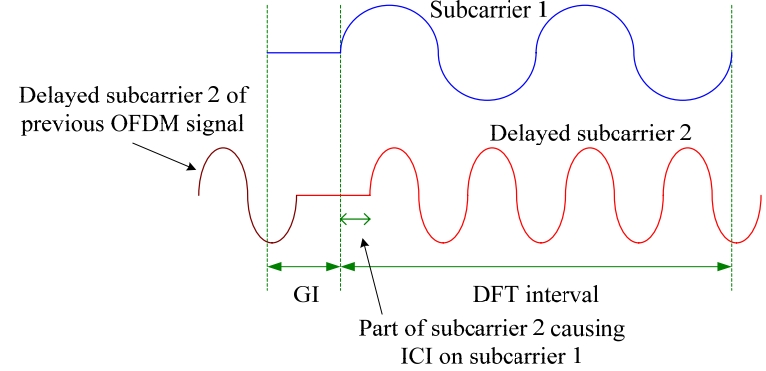
\includegraphics[width=0.5\textwidth]{GI.jpg}
    \end{figure}
    \begin{itemize}
        \item In DFT interval, difference between two subcarriers does not  maintain integer number of cycles    $ \rightarrow$ loss of orthogonality.
        \item Delayed version of subcarrier 2 causes ICI in the process of  demodulating subcarrier 1.
    \end{itemize}
\end{frame}
%-----------------------------------------------------------------------------%
\begin{frame}
    \frametitle{Cyclic Prefix(3/13)}
    \begin{itemize}
        \item Cyclic prefix (CP):A copy of the last part of OFDM signal is attached to the front of itself.
    \end{itemize}
    \begin{figure}
        \centering
        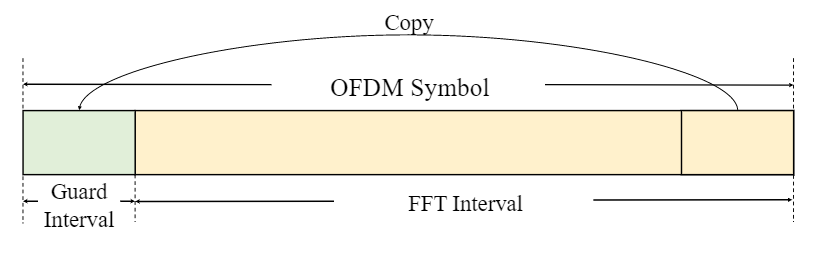
\includegraphics[width=0.4\textwidth]{CP_9.png}
    \end{figure}
    \begin{itemize}
        \item All delayed replicas of subcarriers always have an integer number of cycles within DFT interval, which means no ICI.
    \end{itemize}
    \begin{figure}
        \centering
        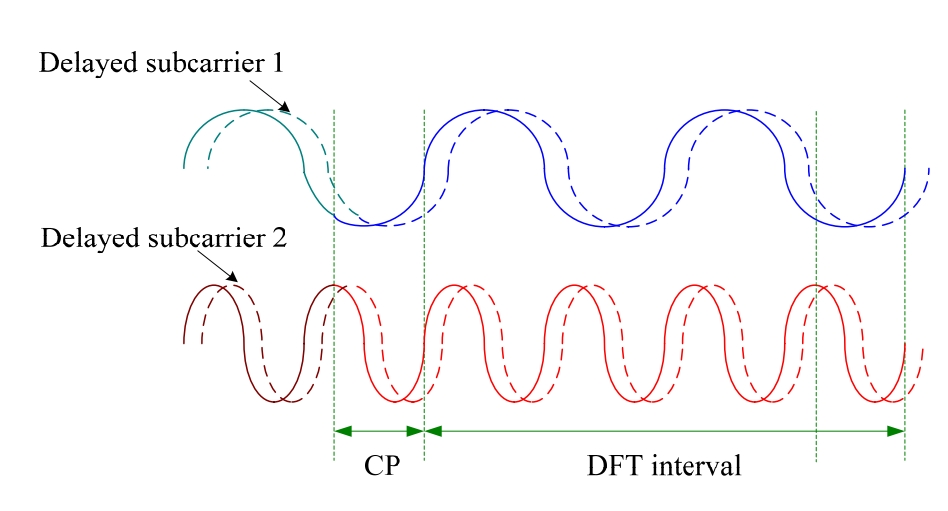
\includegraphics[width=0.4\textwidth]{delay.jpg}
    \end{figure}
\end{frame}
%-----------------------------------------------------------------------------%
\begin{frame}
    \frametitle{Cyclic Prefix(4/13)}
    \begin{itemize}
        \item Within the DFT interval, if a subcarrier does not complete an integer number of cycles, its orthogonality is lost, leading to ICI.
    \end{itemize}
    \begin{figure}
        \centering
        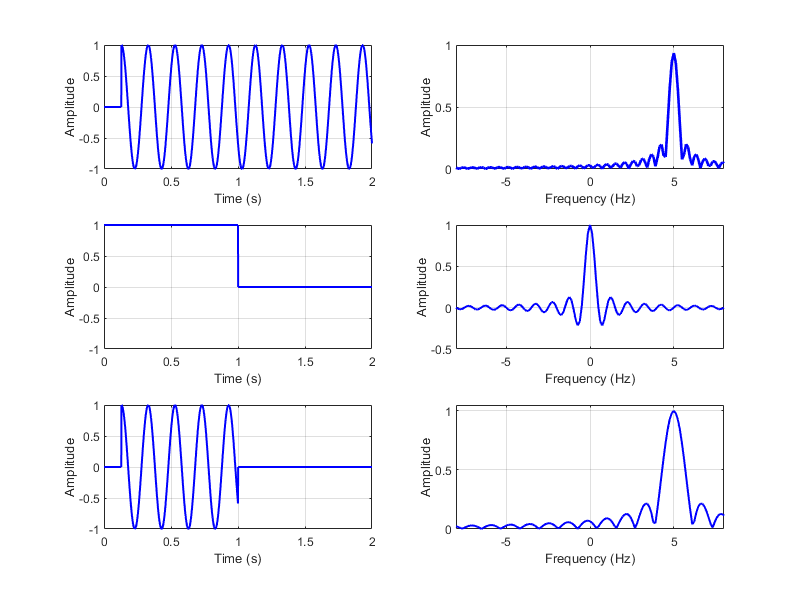
\includegraphics[width=0.75\textwidth]{GI_cause_ISI_modify.png}
    \end{figure}
\end{frame}
%-----------------------------------------------------------------------------%
\begin{frame}
    \frametitle{Cyclic Prefix(5/13)}
    \begin{itemize}
    \item Original continuous subcarrier:
    \begin{align*}
        x(t) &= e^{j 2\pi f_0 t},\, -\infty < t < \infty \\
        X(f) &= \delta(f - f_0)
    \end{align*}
    \item Guard interval of duration $T_{\mathrm{GI}}$:
    \[
        a(t) = 
        \begin{cases}
            1, & T_{\mathrm{GI}} \le t \le T_{\mathrm{GI}}+T \\
            0, & \text{otherwise}
        \end{cases}
    \]
    \[
        A(f) = T \, \mathrm{sinc}(fT)\, e^{-j2\pi f (T_{\mathrm{GI}} + T/2)}.
    \]
    \item Subcarrier with GI:
    \begin{align*} 
        \hat{x}(t) &= a(t)\,e^{j2\pi f_0 t} \\
        \hat{X}(f) &= A(f) * \delta(f-f_0) = A(f-f_0).
    \end{align*}
    Due to GI, the spectrum becomes a shifted sinc (not a perfect delta).
\end{itemize}
\end{frame}
%-----------------------------------------------------------------------------%
\begin{frame}
    \frametitle{Cyclic Prefix(6/13)}
    \begin{itemize}
        \item Linear convolution vs. Circular convolution
    \end{itemize}
    \begin{figure}
        \centering
        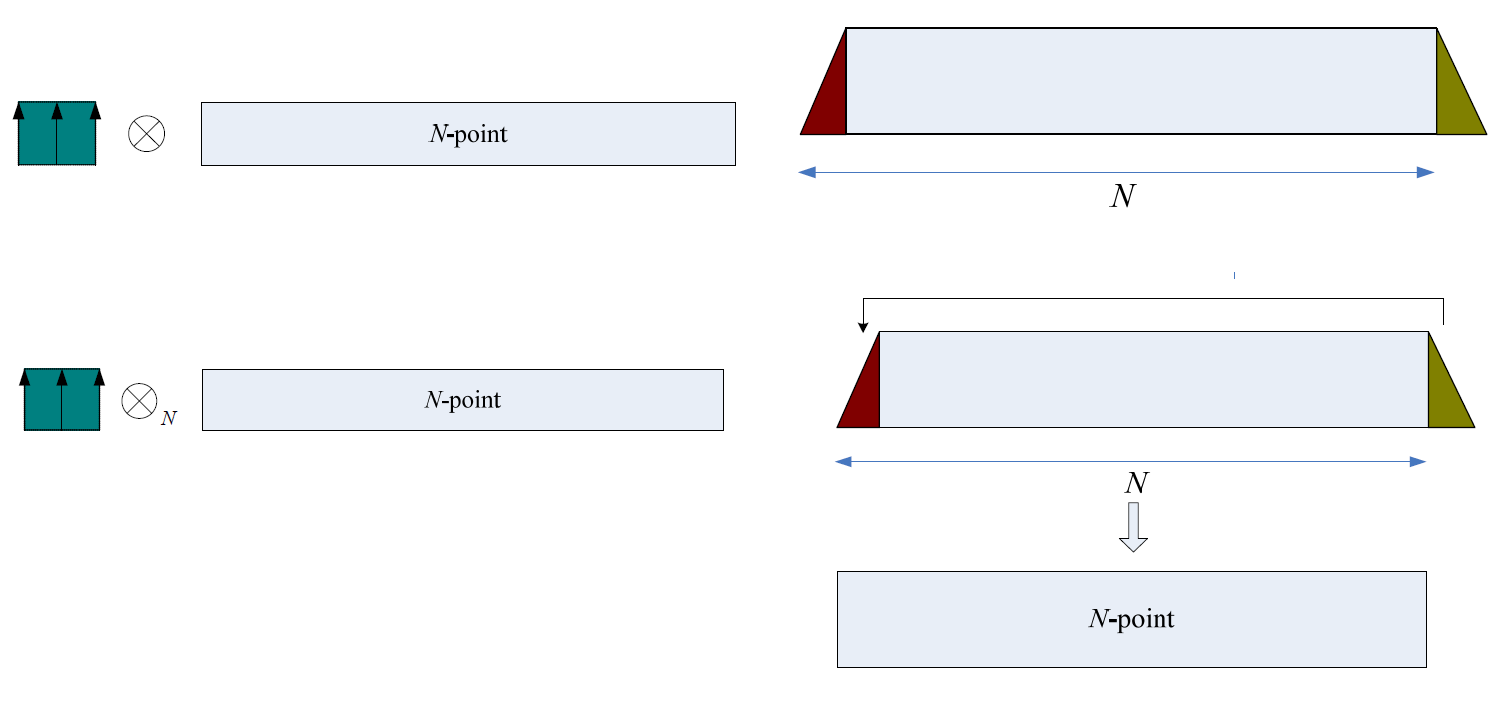
\includegraphics[width=0.7\textwidth]{CP_6.png}
    \end{figure}
\end{frame}
%-----------------------------------------------------------------------------%
\begin{frame}
    \frametitle{Cyclic Prefix(7/13)}
    \begin{itemize}
        \item Linear convolution vs. Circular convolution
    \end{itemize}
    \begin{figure}
        \centering
        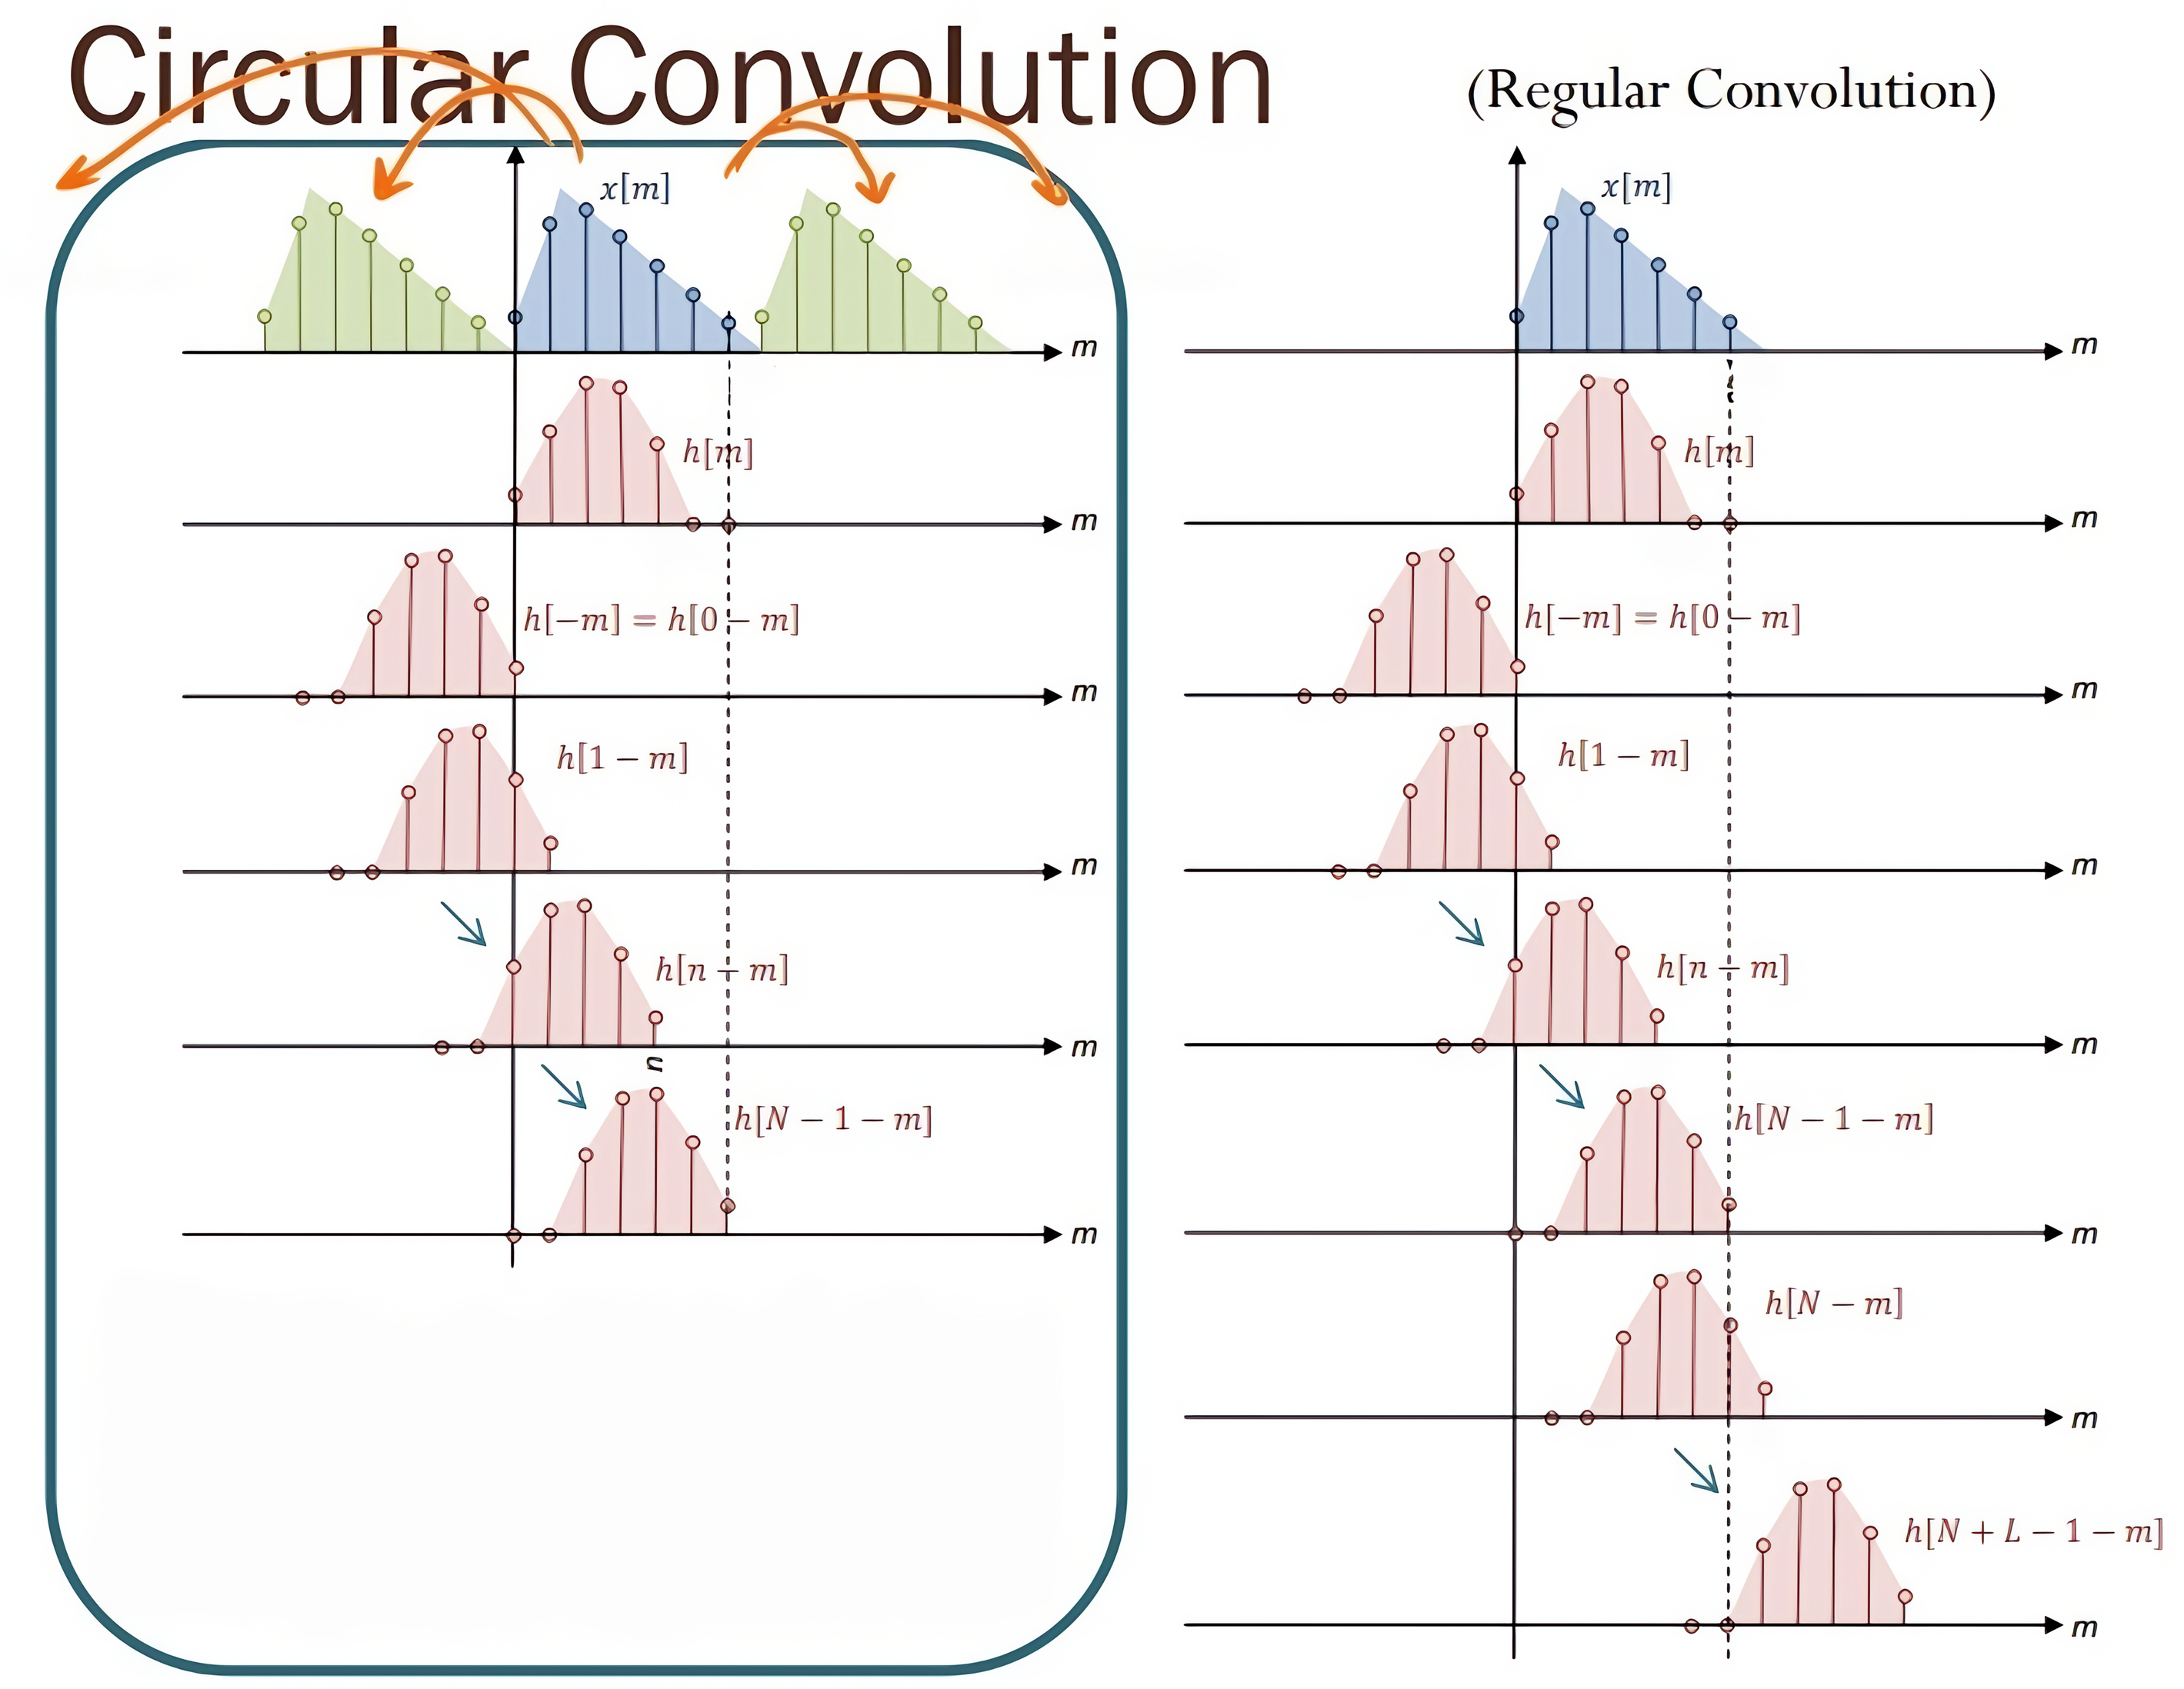
\includegraphics[width=0.65\textwidth]{circular.jpg}
    \end{figure}
\end{frame}
%-----------------------------------------------------------------------------%
\begin{frame}
    \frametitle{Cyclic Prefix(8/13)}
    \begin{itemize}
        \item Linear convolution vs Circular convolution 
    \end{itemize}
    \begin{figure}
        \centering
        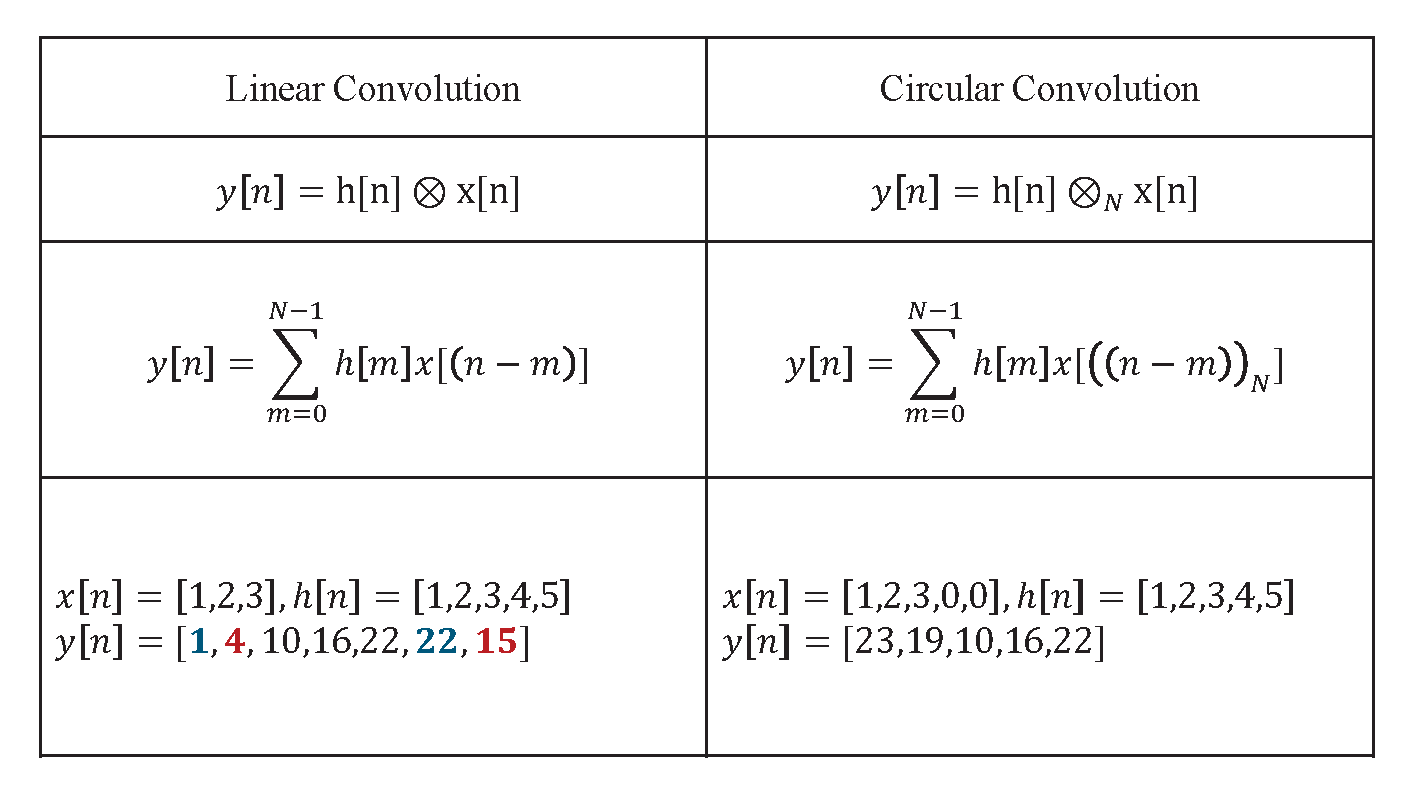
\includegraphics[width=0.8\textwidth]{Linear_convolution_vs_Circular_convolution.eps}
  \end{figure}
\end{frame}
%-----------------------------------------------------------------------------%
\begin{frame}
    \frametitle{Cyclic Prefix(9/13)}
    \begin{itemize}
        \item Channel effect with cyclic prefix
    \end{itemize} 
    \begin{figure}
        \centering
        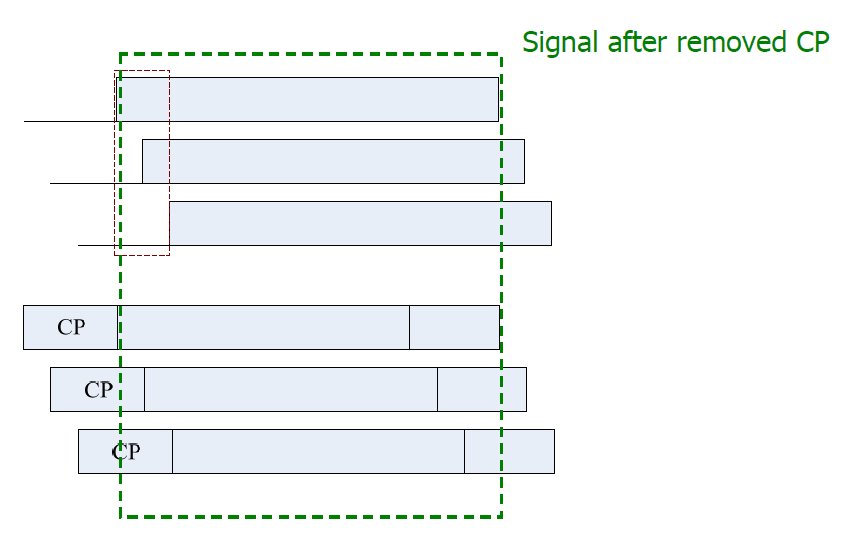
\includegraphics[width=0.8\textwidth]{CP_7.png}
    \end{figure}   
\end{frame}
%-----------------------------------------------------------------------------%
\begin{frame}
  \frametitle{Cyclic Prefix(10/13)}
  \begin{itemize}
    \item Spectrum of channel $h[n]$ response with length $L_{h}$ (smaller than $N_{g}$ )\\
    $H_{k}=\mathrm{FFT}\{h[n]\}$\\
    \item Received complete OFDM signal\\
    $\tilde{r}[n]=\tilde{D}[n]\bigotimes h[n]$, $0\leq n\leq N+N_{g}+L_{h}-2$\\
    \item Received useful part $r[n]$\\
    $r[n]=D[n]\bigotimes_{N}h[n]$\\
    where $\bigotimes_{N}$is N-point circular convolution (due to CP)\\
    \item Received symbol at k-th subcarrier\\
    $Y_{k}=\mathrm{FFT}\{r[n]\}=\mathrm{FFT}\{D[n]\bigotimes_{N}h[n]\}=X_{k}H_{k}$\\
    \( \Rightarrow X_{k} = \frac{Y_{k}}{H_{k}} \)\\
    “Useful property for OFDM system to reduce complexity of channel equalization”.
  \end{itemize}
\end{frame}
%-----------------------------------------------------------------------------%
\begin{frame}
    \frametitle{Cyclic Prefix(11/13)}
    \begin{figure}
    \centering
    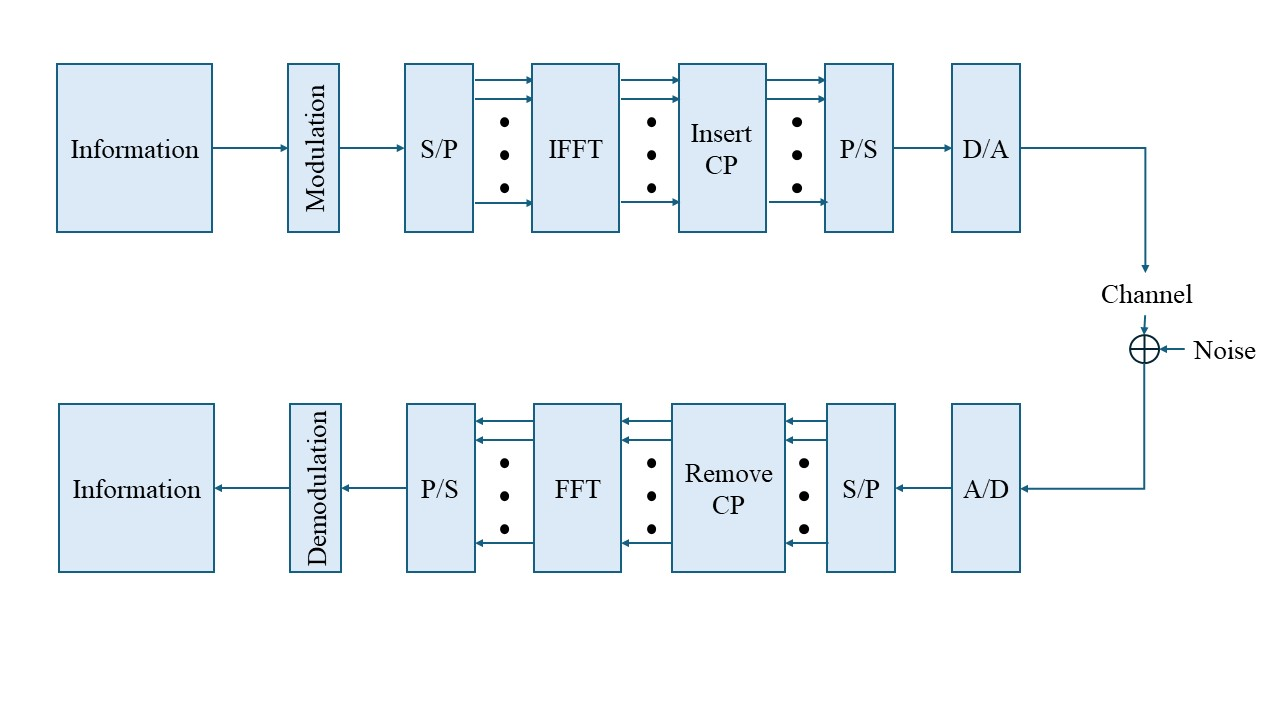
\includegraphics[width=0.9\textwidth]{block_diagram.jpg}
    \end{figure} 
\end{frame}
%-----------------------------------------------------------------------------%
\begin{frame}
    \frametitle{Cyclic Prefix(12/13)}
    \begin{itemize}
        \item Remove Cyclic Prefix
    \end{itemize}
    \begin{figure}
        \centering
        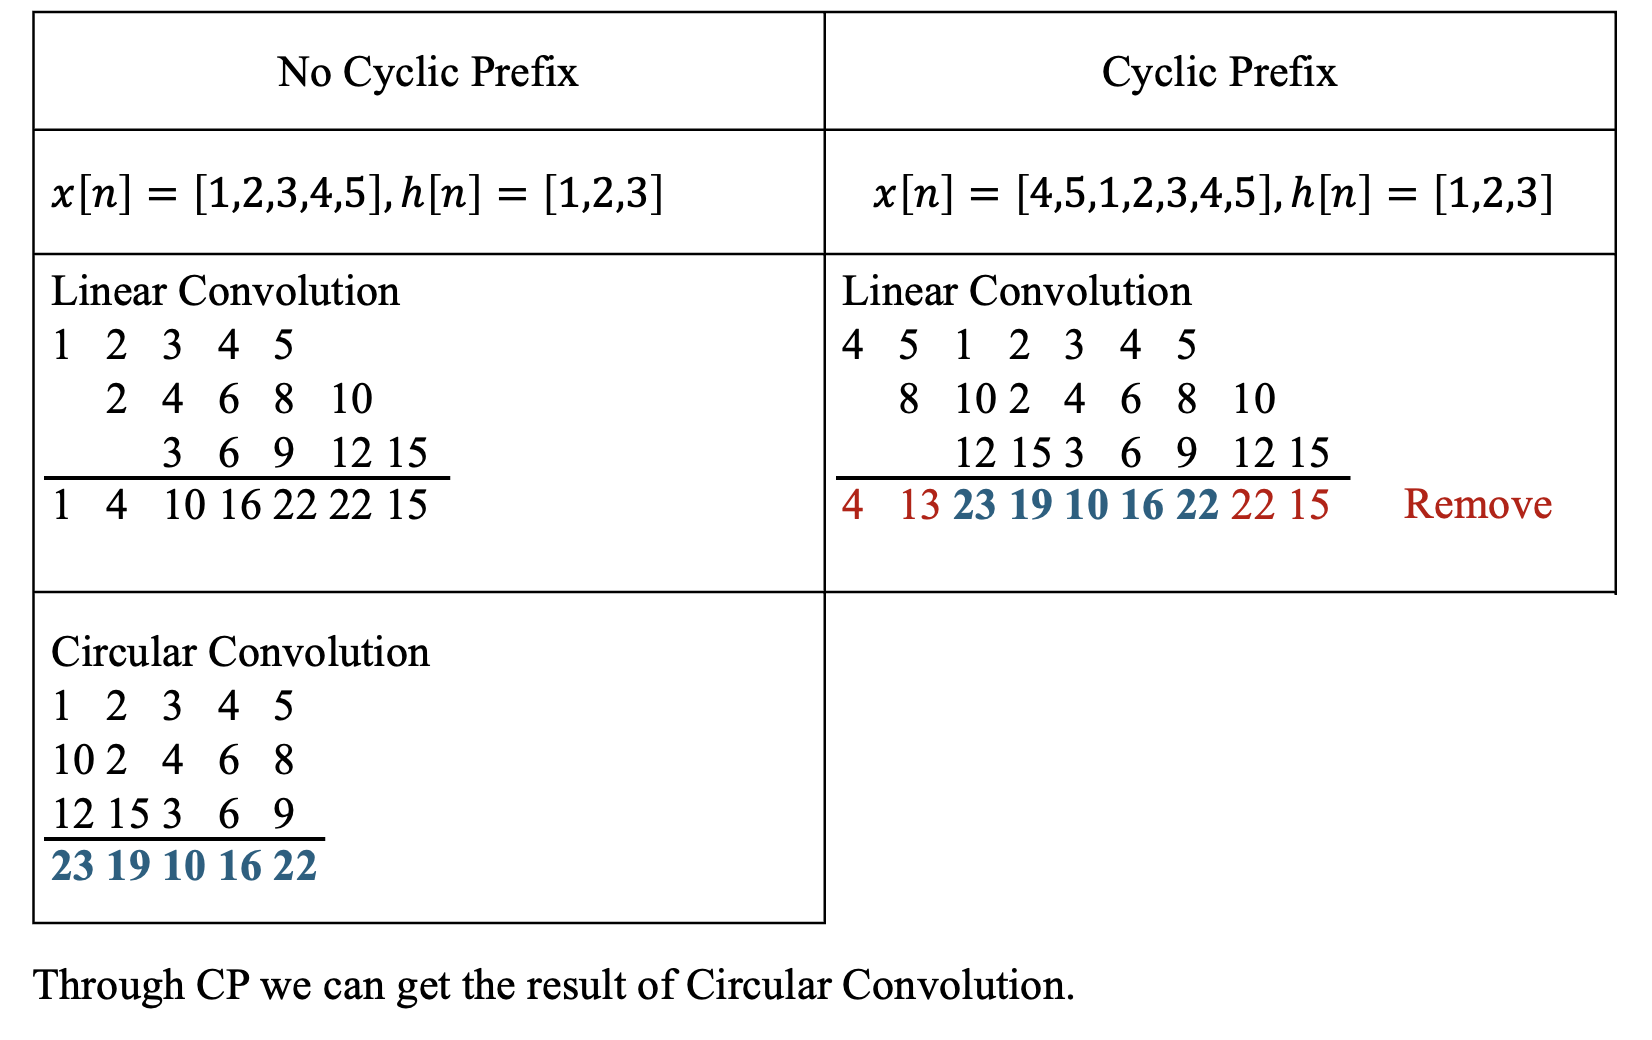
\includegraphics[width=0.85\textwidth]{cp12.png}
    \end{figure}
\end{frame}
%-----------------------------------------------------------------------------%
\begin{frame}
    \frametitle{Cyclic Prefix(13/13)}
    \begin{itemize}
        \item One of the most important reasons to do OFDM is the efficient way it deals with multipath delay spread.
        \item To eliminate inter-symbol interference (ISI) almost completely, a CP duration time ($\Delta$) is introduced for each OFDM symbol.\\
        (The CP duration time is chosen larger than the maximum delay spread ($\tau$))
    \end{itemize}
    \begin{figure}
        \centering
        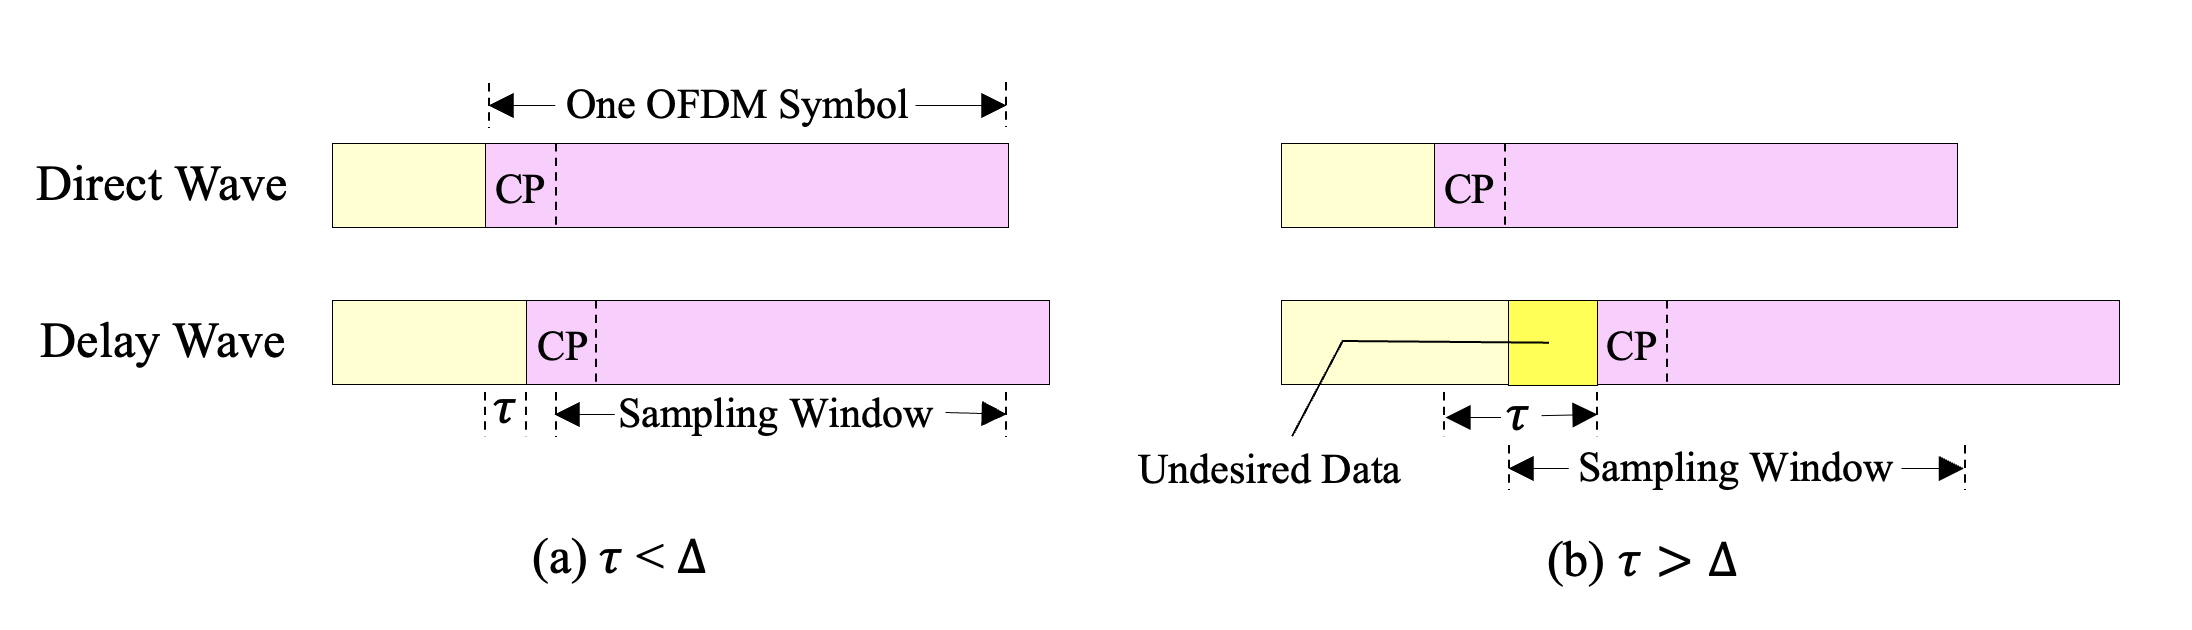
\includegraphics[width=0.85\textwidth]{cp11.png}
    \end{figure}
\end{frame}
%-----------------------------------------------------------------------------%
\begin{frame}
    \frametitle{Bandwidth Efficiency}
    \begin{itemize}
        \item In a classical parallel system, the channel is divided into
            N non-overlapping sub-channels to avoid inter-carrier interference (ICI).
        \item The diagram for bandwidth efficiency of OFDM system is shown below:
        \begin{figure}
            \centering
            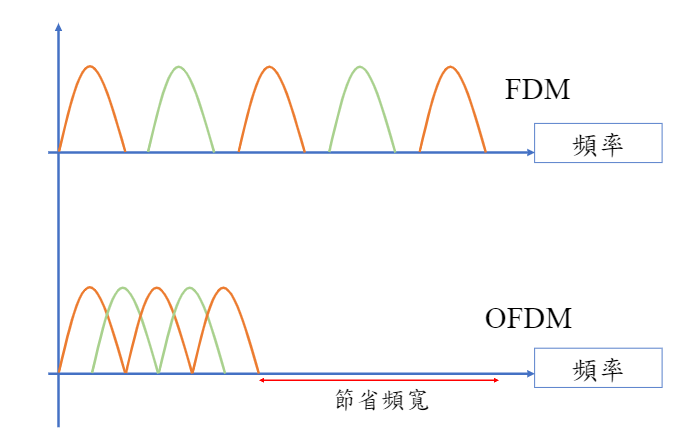
\includegraphics[width=0.6\textwidth]{CP_8.png}
        \end{figure}
    \end{itemize}
\end{frame}
%-----------------------------------------------------------------------------%
\begin{frame}
    \frametitle{Summary}
    \begin{itemize}
        \item The advantage of the FFT-based OFDM system:
        \begin{itemize}
            \item The use of IFFT/FFT can reduce the computation complexity.
            \item The orthogonality between the adjacent sub-carriers will make the use of transmission bandwidth more efficient.
            \item The guard interval is used to resist the inter-symbol interference (ISI).
            \item The main advantage of the OFDM transmission technique is its high performance even in frequency selective channels.
        \end{itemize}
    \end{itemize}
    \begin{itemize}
        \item The drawbacks of the OFDM system :
        \begin{itemize}
            \item It is highly vulnerable to synchronization errors.
            \item Peak to Average Power Ratio (PAPR) problems
            \[
                \hspace{-1.5cm} PAPR = \frac{max.\ power\ of\ subcarriers}{avg.\ power\ of\ subcarriers}
            \]
        \end{itemize}
    \end{itemize}
\end{frame}
%-----------------------------------------------------------------------------%
\begin{frame}
\frametitle{Appendix}
\begin{itemize}
  \item Coherent Bandwidth\\
  \begin{itemize}
    \item Spaced-frequency correlation function:
    \begin{equation*}
        R(\Delta f) = E\big[H(f,t)\,H^{*}(f+\Delta f,\,t)\big]
    \end{equation*}
    \item Coherence Bandwidth is defined as the value of $\Delta f$ for which $|R(\Delta f)|$ is above a certain threshold (e.g., 0.5 or 0.9).
    \begin{equation*}
    B_c \approx \Delta f \quad \text{s.t.} \quad |R(\Delta f)| = \text{threshold}
    \end{equation*}
  \end{itemize}
\end{itemize}
\end{frame}
%-----------------------------------------------------------------------------%
\begin{frame}
\frametitle{Appendix}
\begin{itemize}
  \item Proof\ \ \ \textbf{$Y_{k}=X_{k}H_{k}$}\\
  \begin{itemize}
    \item Using the definition of the DFT:
    \[X_{k} = DFT\bigg\{x[n]\bigg\} = \sum_{n=0}^{N-1}x[n]e^\frac{-j2{\pi}kn}{N}\]
  \[x[n] = IDFT\bigg\{X_{k}\bigg\} = \frac{1}{N}\sum_{k=0}^{N-1}X_{k}e^\frac{j2{\pi}kn}{N}\]
    \item Then, we can write the transform equation for $H_{k}$.
    \[H_{k} = \sum_{m=0}^{N-1}h[m]e^\frac{-j2{\pi}km}{N},\ m=0,1,2,...,N-1\]
  \end{itemize}
\end{itemize}
\end{frame}
%-----------------------------------------------------------------------------%
\begin{frame}
\frametitle{Appendix}
\begin{itemize}
  \item Continued from previous page: 
  \begin{align*}
  Y_{k} & = \bigg[\sum_{n=0}^{N-1}x[n]e^\frac{-j2{\pi}kn}{N}\bigg]\bigg[\sum_{m=0}^{N-1}h[m]e^\frac{-j2{\pi}km}{N}\bigg] \\
  y[n] & =\ \frac{1}{N}\sum_{k=0}^{N-1}\bigg[\sum_{l=0}^{N-1}x[l]e^\frac{-j2{\pi}kl}{N}\bigg]\bigg[\sum_{m=0}^{N-1}h[m]e^\frac{-j2{\pi}km}{N}\bigg]e^\frac{j2{\pi}kn}{N} \\
   & =\ \frac{1}{N}\sum_{l=0}^{N-1}x[l]\sum_{m=0}^{N-1}h[m]\bigg[\sum_{k=0}^{N-1}e^\frac{j2{\pi}k(n-l-m)}{N}\bigg]
\end{align*}
\end{itemize}
\end{frame}
%-----------------------------------------------------------------------------%
\begin{frame}
\frametitle{Appendix}
\begin{itemize}
  \item Now, we see that the item in brackets can be evaluated as
  \begin{equation*}
    \sum_{k=0}^{N-1}e^\frac{j2{\pi}k(n-l-m)}{N} =\begin{cases}
                                                   N, & n-l-m =KN , \text{ for some integer } K \\
                                                   0 , & otherwise
                                                 \end{cases}
  \end{equation*}
  and, therefore
  \[y[n] = \frac{1}{N}\sum_{l=0}^{N-1}x[l]\sum_{m=0}^{N-1}h[m]N\delta[n-l-m-KN]\]
  \[(n-l-m)  \text{ mod N }\equiv  0 \text{ mod N }\]
  Because the impulse function is zero expect when \[m \text{ mod N }\equiv(n-l) \text{ mod N }\], we can rewrite the equation as
  \[y[n] = \sum_{l=0}^{N-1}x[l]h[n-l]_{mod\ N}\]
\end{itemize}
\end{frame}
%-----------------------------------------------------------------------------%
\begin{frame}
\frametitle{Appendix}
\begin{itemize}
    \item Circular Convolution in Time Domain
\[
y[n] = \sum_{m=0}^{N-1} x[m]\, h[(n-m)\bmod N], \qquad n=0,\dots,N-1
\]

Take the DFT of $y[n]$:
\[
\begin{aligned}
Y_k &= \sum_{n=0}^{N-1} y[n]\,e^{-j\frac{2\pi}{N}kn} \\[2mm]
    &= \sum_{n=0}^{N-1}\sum_{m=0}^{N-1} x[m]\;h[(n-m)\bmod N]\;e^{-j\frac{2\pi}{N}kn}.
\end{aligned}
\]
\end{itemize}
\end{frame}
%----------------------------------------------------------------------------%

\begin{frame}
\frametitle{Appendix}
\begin{itemize}
  \item Continued from previous page:
\end{itemize}

\hspace*{2em} 
Let $r=(n-m)\bmod N$ \\

\vspace{1em}

\[
\begin{aligned}
Y_k &= \sum_{m=0}^{N-1} x[m]\;\sum_{r=0}^{N-1} h[r]\;e^{-j\frac{2\pi}{N}k(r+m)} \\[2mm]
    &= \Biggl(\sum_{m=0}^{N-1} x[m]\,e^{-j\frac{2\pi}{N}km}\Biggr)
       \Biggl(\sum_{r=0}^{N-1} h[r]\,e^{-j\frac{2\pi}{N}kr}\Biggr) \\[2mm]
    &= X_k H_k.
\end{aligned}
\]

\vspace{1em}

\[
\boxed{Y_k = X_k H_k}
\]
\end{frame}

%----------------------------------------------------------------------------%





\begin{frame}
\frametitle{Appendix}
\begin{itemize}
  \item Circular convolution:
  \[y[n] = x[n]\bigotimes_{N}h[n] = \sum_{l=0}^{N-1}x[l]h[n-l]_{mod\ N}\]
  As a result, we can get the DFT pair:
  \[y[n]=x[n]\bigotimes_{N}h[n] \leftrightarrow\ Y_{k}=X_{k}H_{k}\] 
\end{itemize}
\end{frame}
%-----------------------------------------------------------------------------%
\begin{frame}
\frametitle{Appendix}
\begin{itemize}
  \item Integrate the Exponential Function
  
  To integrate this, we use the formula for the integral of an exponential function:   
    \[
    \int e^{j\omega t} \, dt = \frac{e^{j\omega t}}{j\omega}
    \]
    Here, \(\omega = 2\pi \frac{p - q}{N\Delta t}\). Applying this to our integral:
    \[
    \int_a^b e^{j2\pi(\frac{p - q}{N\Delta t})t} \, dt = \left[ \frac{e^{j2\pi(\frac{p - q}{N\Delta t})t}}{j2\pi(\frac{p - q}{N\Delta t})} \right]_a^b
    \]
 
\end{itemize}
\end{frame}
%-----------------------------------------------------------------------------%
\begin{frame}
\frametitle{Appendix}
\begin{itemize}
  \item Evaluate the Integral from \(a\) to \(b\)
  
  Substituting the limits \(a\) and \(b\) into the expression:
    \[
    \frac{1}{j2\pi(\frac{p - q}{N\Delta t})} \left( e^{j2\pi(\frac{p - q}{N\Delta t})b} - e^{j2\pi(\frac{p - q}{N\Delta t})a} \right)
    \]
\end{itemize}
\end{frame}
%-----------------------------------------------------------------------------%
\begin{frame}
\frametitle{Appendix}
\begin{itemize}
  \item Given that \(b = a + N\Delta t\), substitute this into the expression
  
   \[
    e^{j2\pi \left( \frac{p-q}{N\Delta t} \right) b} = e^{j2\pi \left( \frac{p-q}{N\Delta t} \right) (a + N\Delta t)}
    \]

     Utilizing the property of exponents \(e^{j(\alpha + \beta)} = e^{j\alpha} e^{j\beta}\), we can rewrite the expression as:

     \[
    e^{j2\pi \left( \frac{p-q}{N\Delta t} \right) b} = e^{j2\pi \left( \frac{p-q}{N\Delta t} \right) a} \cdot e^{j2\pi (p-q)}
    \]

\end{itemize}
\end{frame}
%-----------------------------------------------------------------------------%
%-----------------------------------------------------------------------------%
\begin{frame}
\frametitle{Appendix}
\begin{itemize}
  \item Since \(p - q\) is an integer, \(e^{j2\pi (p-q)} = 1\). This is due to the periodic nature of the complex exponential function, where the result returns to 1 every time the angle is a multiple of \(2\pi\)
  
    \[
    e^{j2\pi \left( \frac{p-q}{N\Delta t} \right) b} = e^{j2\pi \left( \frac{p-q}{N\Delta t} \right) a}
    \]

    substitute these results back into the integral expression
    \[
    \frac{1}{j2\pi \left( \frac{p-q}{N\Delta t} \right)} \left( e^{j2\pi \left( \frac{p-q}{N\Delta t} \right) a} \cdot e^{j2\pi (p-q)} - e^{j2\pi \left( \frac{p-q}{N\Delta t} \right) a} \right)
    \]


    Rearranging terms:

     \[
    \frac{1}{j2\pi \left( \frac{p-q}{N\Delta t} \right)} \left( e^{j2\pi \left( \frac{p-q}{N\Delta t} \right) a} \cdot (1 - 1) \right)
    \]


\end{itemize}
\end{frame}
%-----------------------------------------------------------------------------%
\begin{frame}
\frametitle{Appendix}
\begin{itemize}
  \item Result
  
  Since \(e^{j2\pi (p-q)} = 1\), we have \(1 - 1 = 0\). Thus, the entire expression ultimately simplifies to:


    \[
    \frac{1}{j2\pi \left( \frac{p-q}{N\Delta t} \right)} \cdot 0 = 0
    \]

\end{itemize}
\end{frame}


%-----------------------------------------------------------------------------%
\begin{frame}
\frametitle{Appendix}
\setlength{\itemsep}{8pt}
\begin{itemize}
          
    \item The Mixed-Radix Cooley-Tukey algorithm
    \begin{itemize}
        \setlength{\itemsep}{4pt}
        \item Ideal for lengths that are not powers of two, it efficiently handles composite lengths.
        \item Breaking down a DFT of size $N = N_1 \times N_2$ into smaller DFTs of sizes $N_1$ and $N_2$.
        \item The algorithm reduces the time complexity from \(O(N^2)\) to \(O\left(N_1 \times N_2 \times (N_1 + N_2)\right) = O(N \times (N_1 + N_2))\).
    \end{itemize}
 
\end{itemize}
\end{frame}

%-----------------------------------------------------------------------------%
\begin{frame}
    \frametitle{Appendix}
    \begin{itemize}
        \item Mixed-Radix Cooley-Tukey Algorithm: \(N = 21, N_1 = 7, N_2 = 3\)
    \end{itemize} 
    \begin{figure}
        \centering
        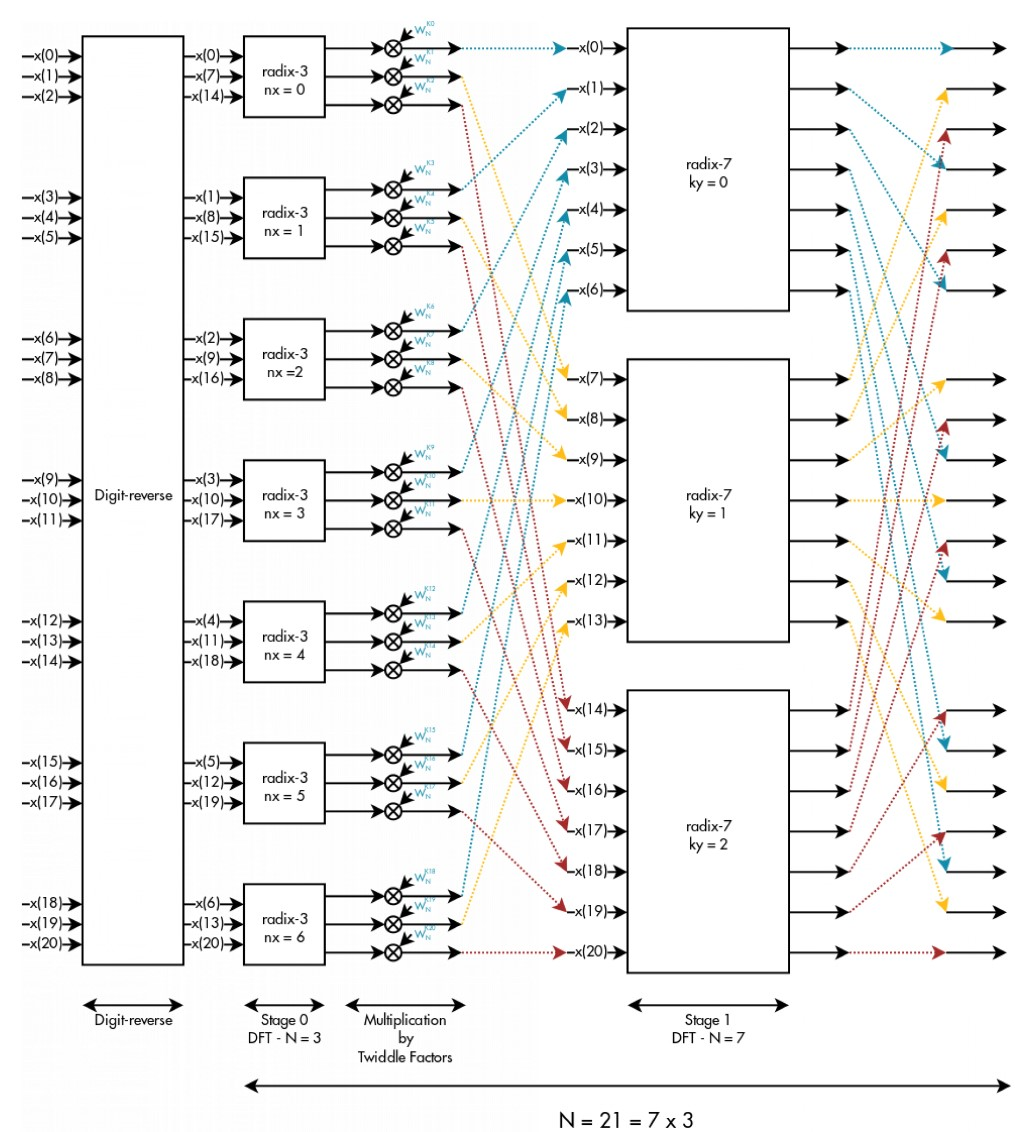
\includegraphics[width=0.57\textwidth, trim=0cm 1cm 0cm 0.4cm, clip]{ifft_21.jpg}
    \end{figure}   
\end{frame}

%-----------------------------------------------------------------------------%
\begin{frame}
\frametitle{Appendix}
    \begin{itemize}
    \item The Mixed-Radix Cooley-Tukey algorithm is defined as the DFT:    
    %\resizebox{0.9\textwidth}{!}{
    %\begin{minipage}{\textwidth}
            \[
            X_k = \sum_{n=0}^{N-1} x_n e^{-\frac{2\pi i}{N}nk} \quad \text{for} \quad k = 0, \dots, N-1
            \]

            Given that \(N = N_1 \cdot N_2\)

            Substituting \(n = n_1 + n_2 N_1\) and \(k = k_1 N_2 + k_2\), we have:
            \begin{align*}
            e^{-\frac{2\pi i}{N} nk} &= e^{-\frac{2\pi i}{N} (n_1 + n_2 N_1)(k_1 N_2 + k_2)} \\
                                     &= e^{-\frac{2\pi i}{N} n_1 k_1 N_2} e^{-\frac{2\pi i}{N} n_1 k_2} e^{-\frac{2\pi i}{N} n_2 N_1 k_1 N_2} e^{-\frac{2\pi i}{N} n_2 N_1 k_2} \\
                                     &= e^{-\frac{2\pi i}{N_1} n_1 k_1 } e^{-\frac{2\pi i}{N} n_1 k_2} e^{-\frac{2\pi i}{N_2} n_2 k_2}
            \end{align*}
    %\end{minipage}}
    \end{itemize}
    \begin{itemize}
    \item The Mixed-Radix Cooley-Tukey Algorithm:
            \[
            X_{k_1 N_2 + k_2} = \sum_{n_1=0}^{N_1-1} \left( \sum_{n_2=0}^{N_2-1} \left( x_{n_1 + n_2 N_1} e^{-\frac{2\pi i}{N_2} n_2 k_2} \right) e^{-\frac{2\pi i}{N} n_1 k_2} e^{-\frac{2\pi i}{N_1} n_1 k_1} \right)
            \]      
    \end{itemize}
\end{frame} 

%-----------------------------------------------------------------------------%
\begin{frame}
    \frametitle{Appendix}
        \begin{itemize}
        \item The Example of Cooley-Tukey Algorithm:    
        %\resizebox{0.9\textwidth}{!}{
        %\begin{minipage}{\textwidth}
    
                Given that \(N = 15, N_1 = 3, N_2 = 5\)
    
                Substituting \(n = n_1 + 3n_2\) and \(k = 5k_1 + k_2\), we have:
                \begin{align*}
                e^{-\frac{2\pi i}{N} nk} &= e^{-\frac{2\pi i}{15} (n_1 + 3n_2)(5k_1 + k_2)} \\
                                         &= e^{-\frac{2\pi i}{15} 5n_1 k_1 } e^{-\frac{2\pi i}{15} n_1 k_2} e^{-\frac{2\pi i}{15} 15n_2 k_1} e^{-\frac{2\pi i}{15} 3n_2 k_2} \\
                                         &= e^{-\frac{2\pi i}{3} n_1 k_1 } e^{-\frac{2\pi i}{15} n_1 k_2} e^{-\frac{2\pi i}{5} n_2 k_2}
                \end{align*}
        %\end{minipage}}
        \end{itemize}
        \begin{itemize}
        \item The Mixed-Radix Cooley-Tukey Algorithm:
                \[
                X_{5k_1 + k_2} = \sum_{n_1=0}^{3-1} \left( \sum_{n_2=0}^{5-1} \left( x_{n_1 + 3n_2} e^{-\frac{2\pi i}{5} n_2 k_2} \right) e^{-\frac{2\pi i}{15} n_1 k_2} e^{-\frac{2\pi i}{3} n_1 k_1} \right)
                \]      
        \end{itemize}
    \end{frame} 
%-----------------------------------------------------------------------------%
\begin{frame}
    \frametitle{Appendix: Carrier Frequency Offset (CFO) Results in Inter-Carrier Interference (ICI) (1/4)}
    \begin{itemize}
      \item Frequency offset equation:
        \begin{equation*}
            f_{\text{offset}} = f_c - f_c'
        \end{equation*}
        where:
        \begin{itemize}
            \item $f_c$: subcarrier's frequency of transmitter
            \item $f_c'$: subcarrier's frequency of receiver
        \end{itemize}
    \end{itemize}
\end{frame}
%-----------------------------------------------------------------------------%
\begin{frame}
    \frametitle{Appendix: Carrier Frequency Offset (CFO) Results in Inter-Carrier Interference (ICI) (2/4)}
    \begin{itemize}
      \item CFO:
      \begin{equation*}
        \epsilon = \frac{f_{\text{offset}}}{\Delta f},\ \Delta f = \frac{1}{N \Delta t}
      \end{equation*}
      \item The offset in the time domain and in the frequency domain:
      \begin{equation*}
        \delta(f - \epsilon)\ \longrightarrow \ \exp(j 2\pi n \epsilon)
      \end{equation*}
      \item Assume no other phase noise, the received signal can be expressed as:\\
      \begin{equation*}
        Y_{l}[n] = \underbrace{\frac{1}{N} \sum_{k=0}^{N-1} H[k]X_{l}[k] e^{j 2\pi n (k+\epsilon)/N}}_{\text{IDFT signal + CFO, l means the l-th subcarrier}} + \underbrace{z_{l}[n]}_{\text{AWGN}}
      \end{equation*}
    \end{itemize}
\end{frame}
%-----------------------------------------------------------------------------%
\begin{frame}
    \frametitle{Appendix: Carrier Frequency Offset (CFO) Results in Inter-Carrier Interference (ICI) (3/4)}
    \begin{figure}
      \centering
      \includegraphics[width=1\textwidth]{CFO_1.png}
    \end{figure}
\end{frame}
%-----------------------------------------------------------------------------%
\begin{frame}
    \frametitle{Appendix: Carrier Frequency Offset (CFO) Results in Inter-Carrier Interference (ICI) (4/4)}
    \begin{itemize}
      \item CFO can be decomposed into integer and fractional parts:
      \begin{equation*}
        \epsilon=\epsilon_{i}+\epsilon_{f}
      \end{equation*}
      \begin{itemize}
        \item $\epsilon_{i}$ is the integer multiple of $\Delta f$ (iCFO/IFO).
        \item $\epsilon_{f}$ is the fractional multiple of $\Delta f$ (fCFO/FFO).
      \end{itemize}
      \item If iCFO exists, carriers are still orthogonal, but BER increases.
      \item If fCFO exists, carriers are not orthogonal, and ICI occurs.
    \end{itemize}
\end{frame}
%-----------------------------------------------------------------------------%
\begin{frame}
    \frametitle{Appendix}
    \begin{itemize}
        \item Consider the real received signal and correlate it with $\psi_{k}(t)$:
        \begin{align*}
            &\int_{a}^{b}  D(t) \psi_{k}^\ast(t)dt \\
            &=\int_{a}^{b} {\Big\{\sum_{n=0}^{N-1}\ a(n)\cos{(2\pi f_{n}t)}+b(n)\sin{(2\pi f_{n}t)}\Big\}} \psi_{k}^\ast(t)dt
        \end{align*}
        \item Sinusoidal carriers with different frequencies are orthogonal to each other.Then
        \begin{align*}    
            =& \int_{a}^{b} [a(k)\cos{(2\pi f_{k}t)}+b(k)\sin{(2\pi f_{k}t)}] \psi_{k}^\ast(t)dt \\
            =&a(k)\int_{a}^{b} \cos{(2\pi f_{k}t)}e^{-j2 \pi f_k t} dt + b(k)\int_{a}^{b} \sin{(2\pi f_{k}t)}e^{-j2 \pi f_k t}dt \\
        \end{align*}
    \end{itemize}
\end{frame}
%-----------------------------------------------------------------------------%
\begin{frame}
    \frametitle{Appendix}
    \begin{itemize}
        \item Continued from previous page:
        \begin{align*}    
            =&a(k)\int_{a}^{b} \cos{(2\pi f_{k}t)}[\cos{(2\pi f_{k}t)} - j\sin{(2\pi f_{k}t)}]dt +\\
            & b(k)\int_{a}^{b} \sin{(2\pi f_{k}t)}[\cos{(2\pi f_{k}t)} - j\sin{(2\pi f_{k}t)}]dt 
        \end{align*}
        \item Sine and cosine carriers at the same frequency are also orthogonal.Then
        \begin{align*}
            =&a(k)\int_{a}^{b} \cos{(2\pi f_{k}t)}^2dt -j b(k)\int_{a}^{b} \sin{(2\pi f_{k}t)}^2dt \\
            &=\frac{a(k)}{2} -j \frac{b(k)}{2}
        \end{align*}
        \item In practice, we take the real part of the correlation with the cosine carrier and the imaginary part with the sine carrier.
    \end{itemize}
\end{frame}
\end{document}  